\section{作用力測定装置の評価実験とその考察}

製作した校正実験装置を用いて行った作用力測定装置の性能評価実験について説明する.

\subsection{実験方法}

作用力測定装置の性能を調べるために,複数の角度からのデータを使用し結果を得る必要があり,
結果の再現性,一般性を確保するためには評価実験を複数回繰り返さなければならない.
大量のデータをプログラムで一度に処理できるようにするため,測定手順を以下のように定めた.

\subsubsection{試行回数と測定角度}
本研究で行った実験についての測定角度および試行回数を以下のTable に示す.

\begin{table}[htbp]
	\begin{center}
		\caption{Experiment conditions}
		\begin{tabular}{|p{30mm}|p{20mm}|p{30}|}
			\hline
			\multicolumn{1}{|c|}{}                  & \multicolumn{1}{|c|}{\textgt{Condition number}} & \multicolumn{1}{|c|}{\textgt{remarks}}          \\ \hline
			\multicolumn{1}{|c|}{Measurement angle} & \multicolumn{1}{|c|}{24}                        & \multicolumn{1}{|c|}{Mesurement every 15 [deg]} \\ \hline
			\multicolumn{1}{|c|}{Number of trials}  & \multicolumn{1}{|c|}{7}                         & \multicolumn{1}{|c|}{}                          \\ \hline
		\end{tabular}
	\end{center}
\end{table}
\subsubsection{測定条件}
\begin{enumerate}[(1)]
	\item サンプリング周期は5[Hz]とする
	\item ロードセルをマイクロステージを用いて 0.03 [mm] ずつ移動させ,ひずみセンサ,\\
	      ロードセルの出力電圧を測定する
	\item 基準を0 [mm]として,0.03 [mm],0.06 [mm],0.09 [mm],0.12 [mm]の計4回移動させる
\end{enumerate}
\subsubsection{測定準備}
\begin{enumerate}[(1)]
	\item 自動回転ステージを用いてロードセルを測定する角度に固定する
	\item 自動一軸ステージを用いてロードセルが供試体に接触する位置を0.01[mm]単位で特定する
	\item 接触する前の位置を基準に測定を開始する
\end{enumerate}
\subsubsection{測定手順}
\begin{enumerate}[(1)]
	\item 測定開始から60秒間待機する
	\item 40秒間の出力電圧の測定
	\item 60秒間の自動ステージ動作時間 (※ 自動ステージ動作後,電圧の安定を図るため)
	\item (2),(3)の作業を5回繰り返す (5回目はロードセル,供試体を非接触状態にする)
\end{enumerate}

\subsection{実験結果}

上述の手順にしたがって,各角度ごとに行った測定結果を以下のFig.~Fig.に示す.
なお,以下に示す結果は1回目の測定結果である.

\begin{figure}[htbp]
    \begin{minipage}[b]{0.45\linewidth}
      \centering
      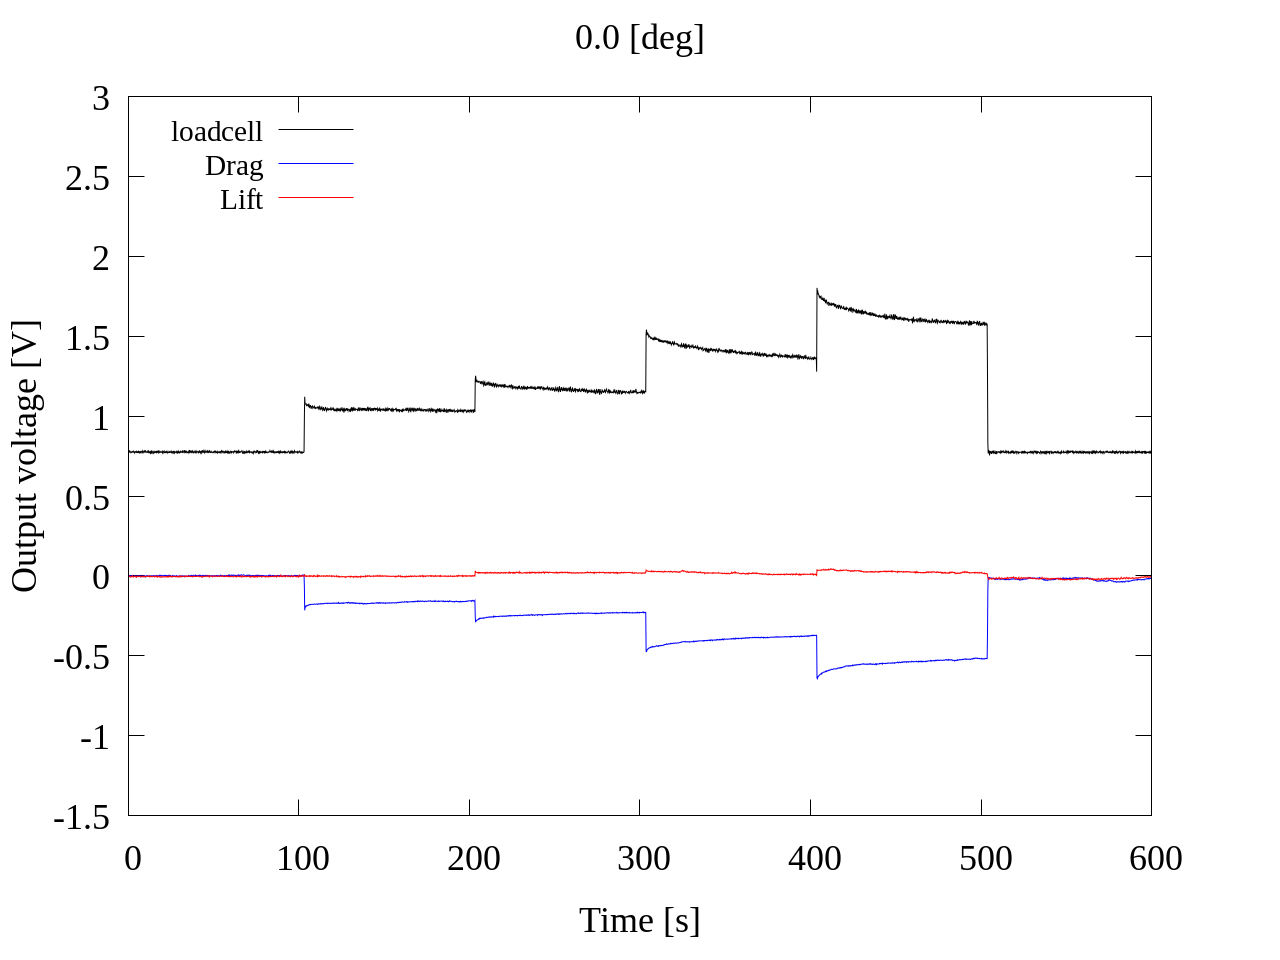
\includegraphics[width=65mm]{../../02_workspace/result/2-1/plot/01-3_allsensors/01_allsensors_0.png}
      \caption{Output voltage : 0 [deg]}
    \end{minipage}
    \begin{minipage}[b]{0.45\linewidth}
      \centering
      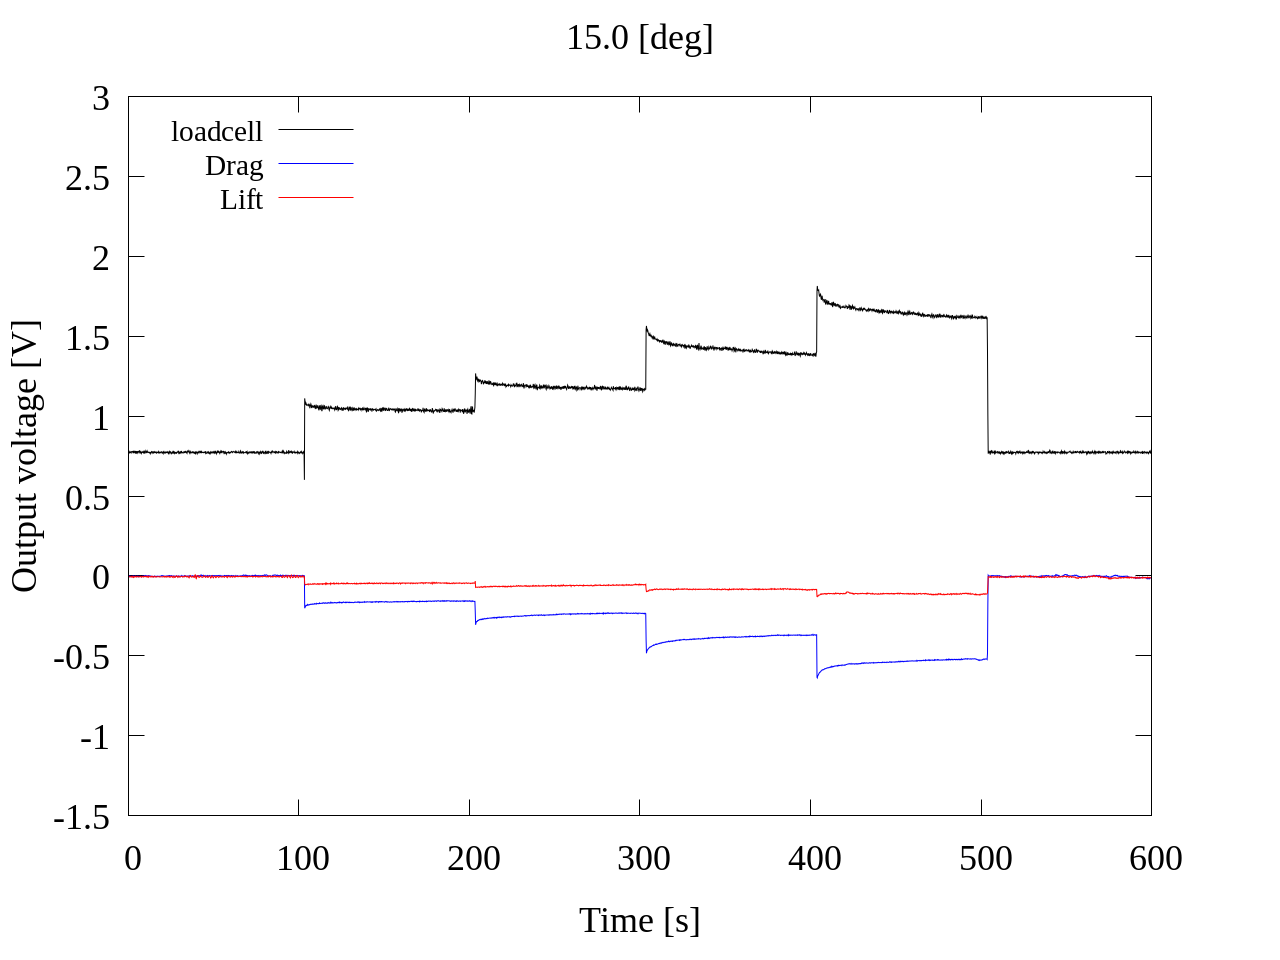
\includegraphics[width=65mm]{../../02_workspace/result/2-1/plot/01-3_allsensors/01_allsensors_150.png}
      \caption{Output voltage : 15 [deg]}
    \end{minipage} \\
    \begin{minipage}[b]{0.45\linewidth}
        \centering
        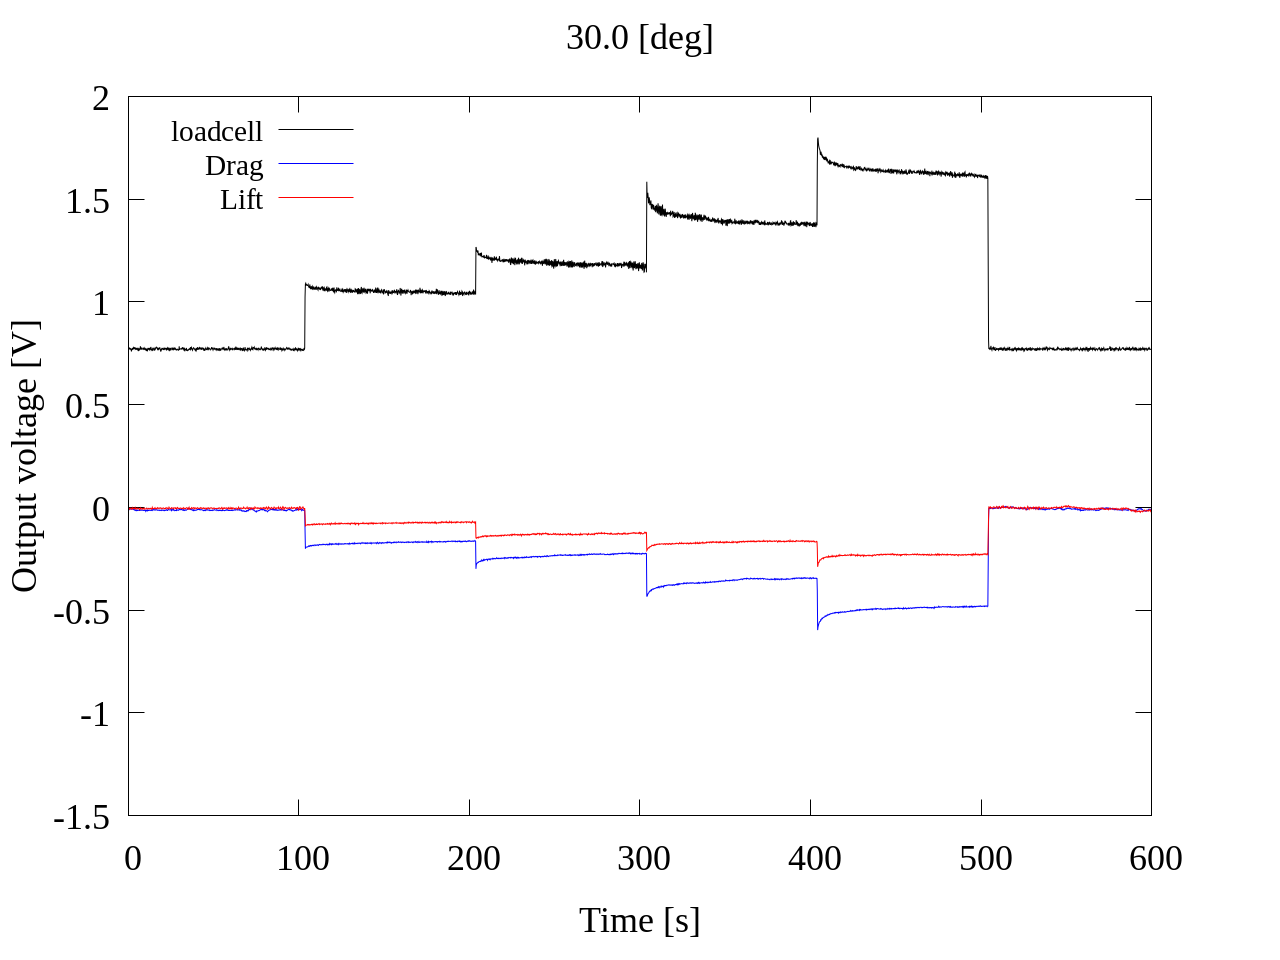
\includegraphics[width=65mm]{../../02_workspace/result/2-1/plot/01-3_allsensors/01_allsensors_300.png}
        \caption{Output voltage : 30 [deg]}
      \end{minipage}
      \begin{minipage}[b]{0.45\linewidth}
        \centering
        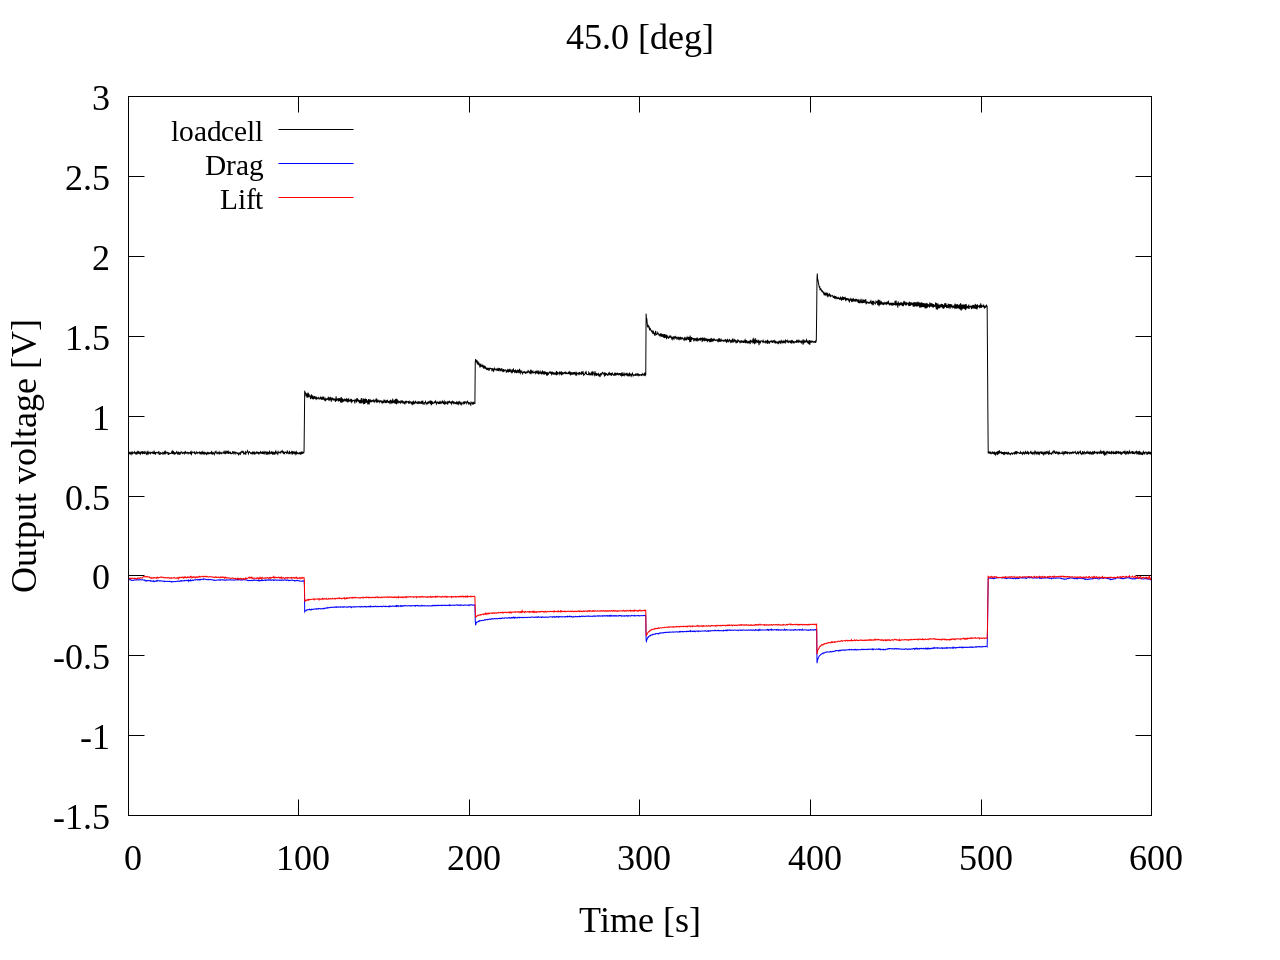
\includegraphics[width=65mm]{../../02_workspace/result/2-1/plot/01-3_allsensors/01_allsensors_450.png}
        \caption{Output voltage : 45 [deg]}
      \end{minipage}\\
      \begin{minipage}[b]{0.45\linewidth}
        \centering
        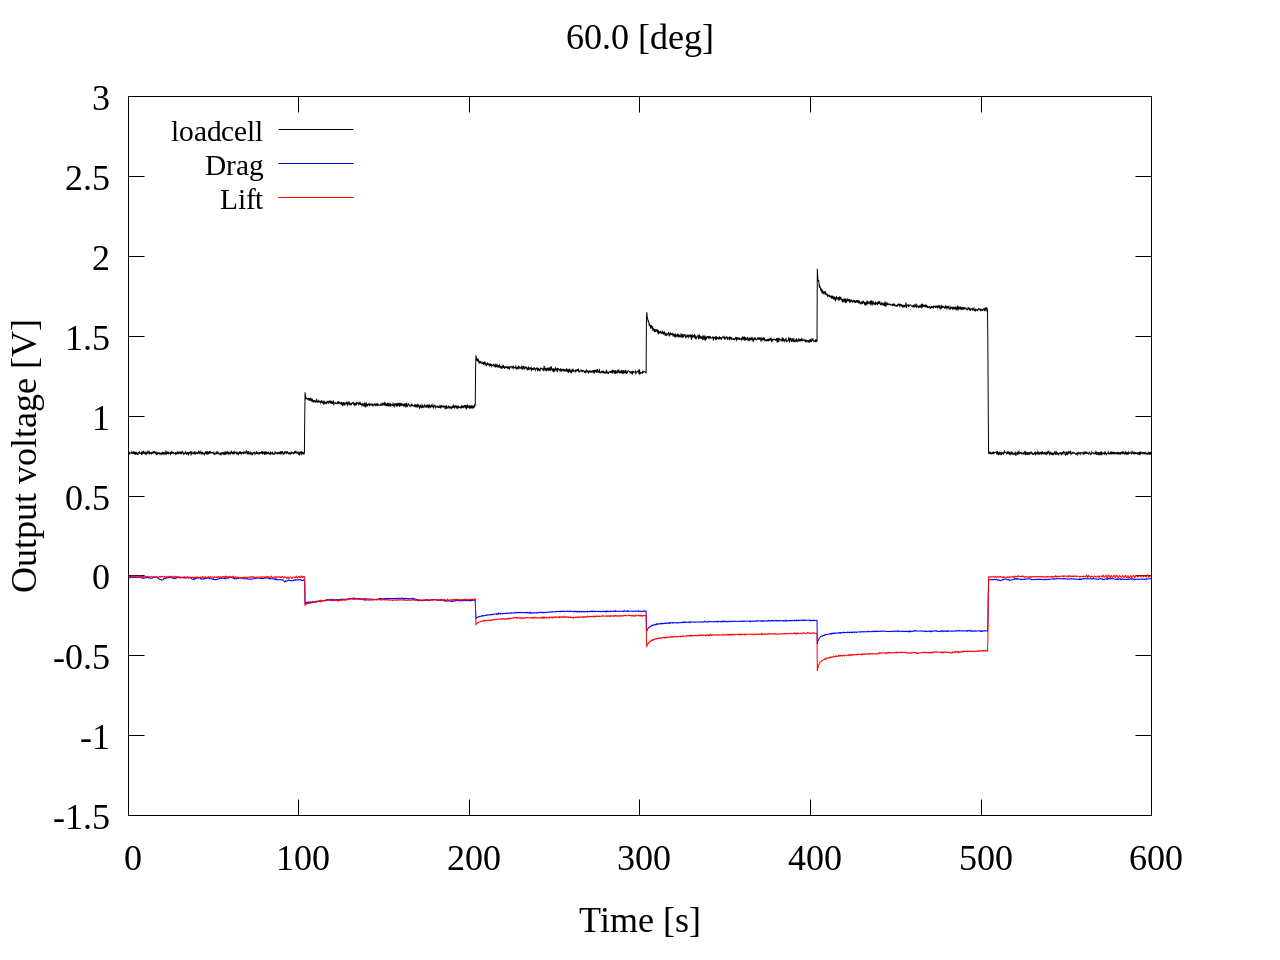
\includegraphics[width=65mm]{../../02_workspace/result/2-1/plot/01-3_allsensors/01_allsensors_600.png}
        \caption{Output voltage : 60 [deg]}
      \end{minipage}
      \begin{minipage}[b]{0.45\linewidth}
        \centering
        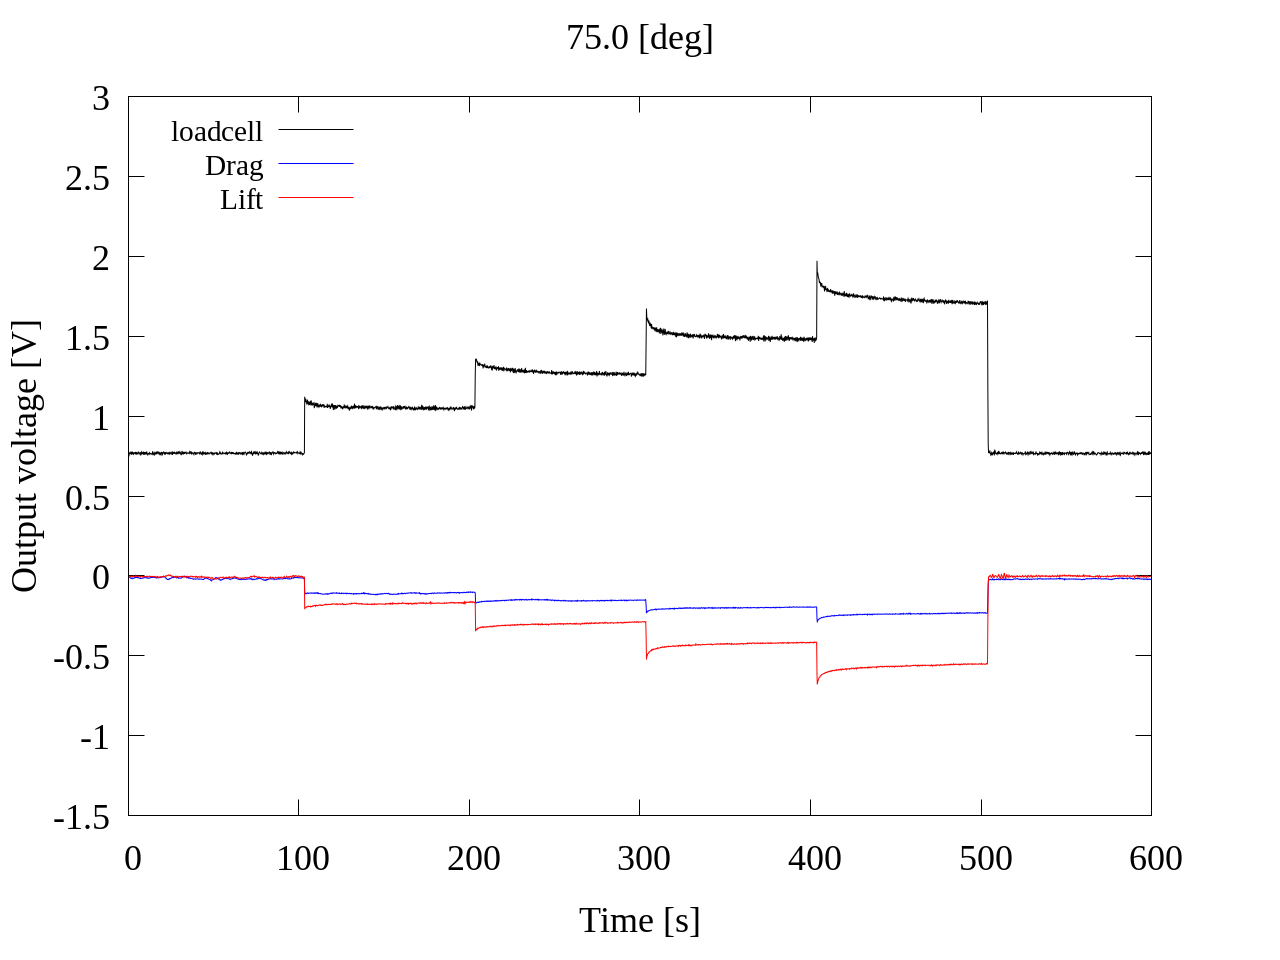
\includegraphics[width=65mm]{../../02_workspace/result/2-1/plot/01-3_allsensors/01_allsensors_750.png}
        \caption{Output voltage : 75 [deg]}
      \end{minipage} 
\end{figure}

\begin{figure}[htbp]
      \begin{minipage}[b]{0.45\linewidth}
        \centering
      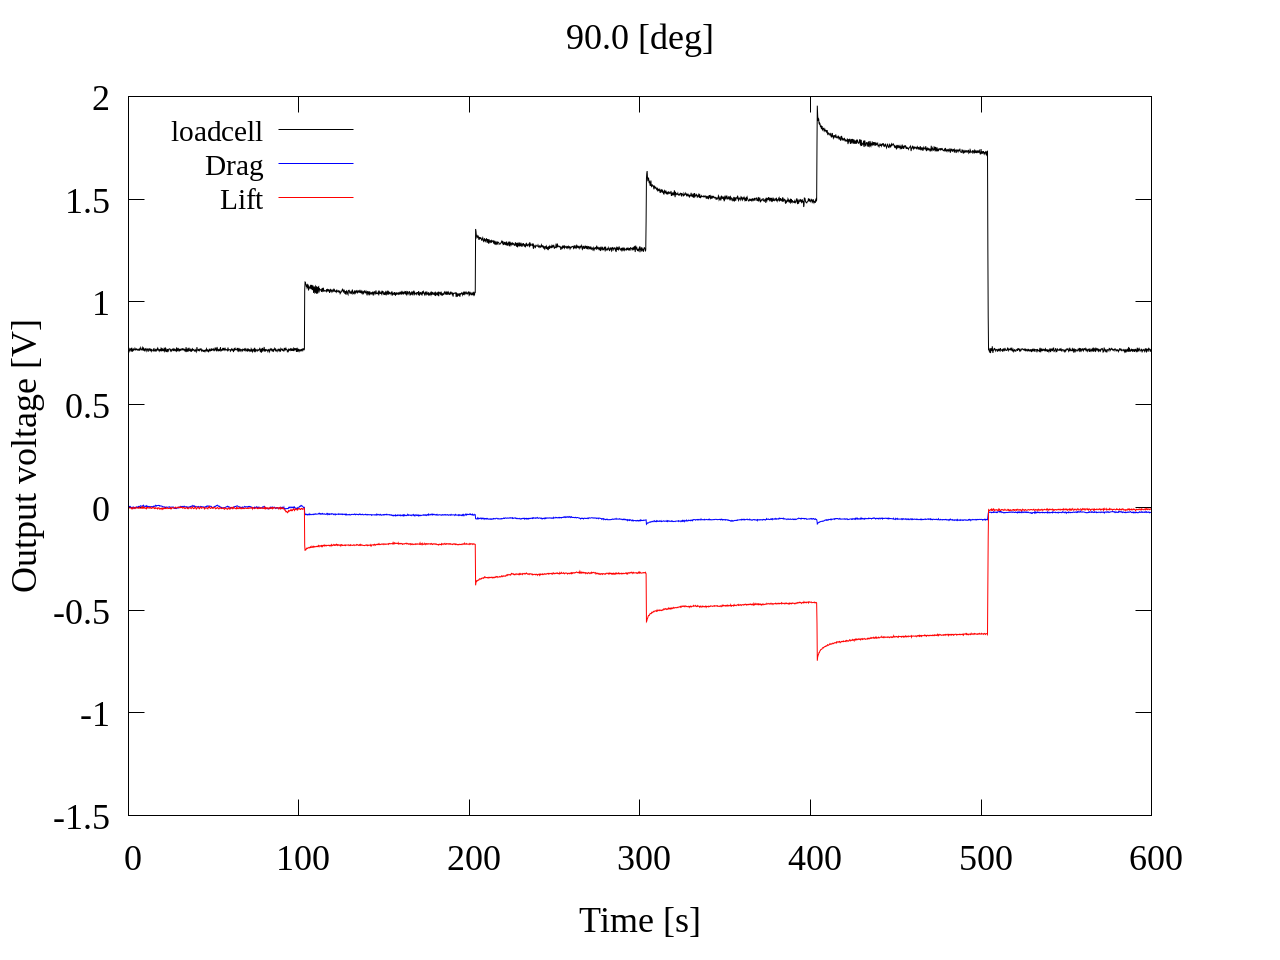
\includegraphics[width=65mm]{../../02_workspace/result/2-1/plot/01-3_allsensors/01_allsensors_900.png}
      \caption{Output voltage : 90 [deg]}
    \end{minipage}
    \begin{minipage}[b]{0.45\linewidth}
        \centering
        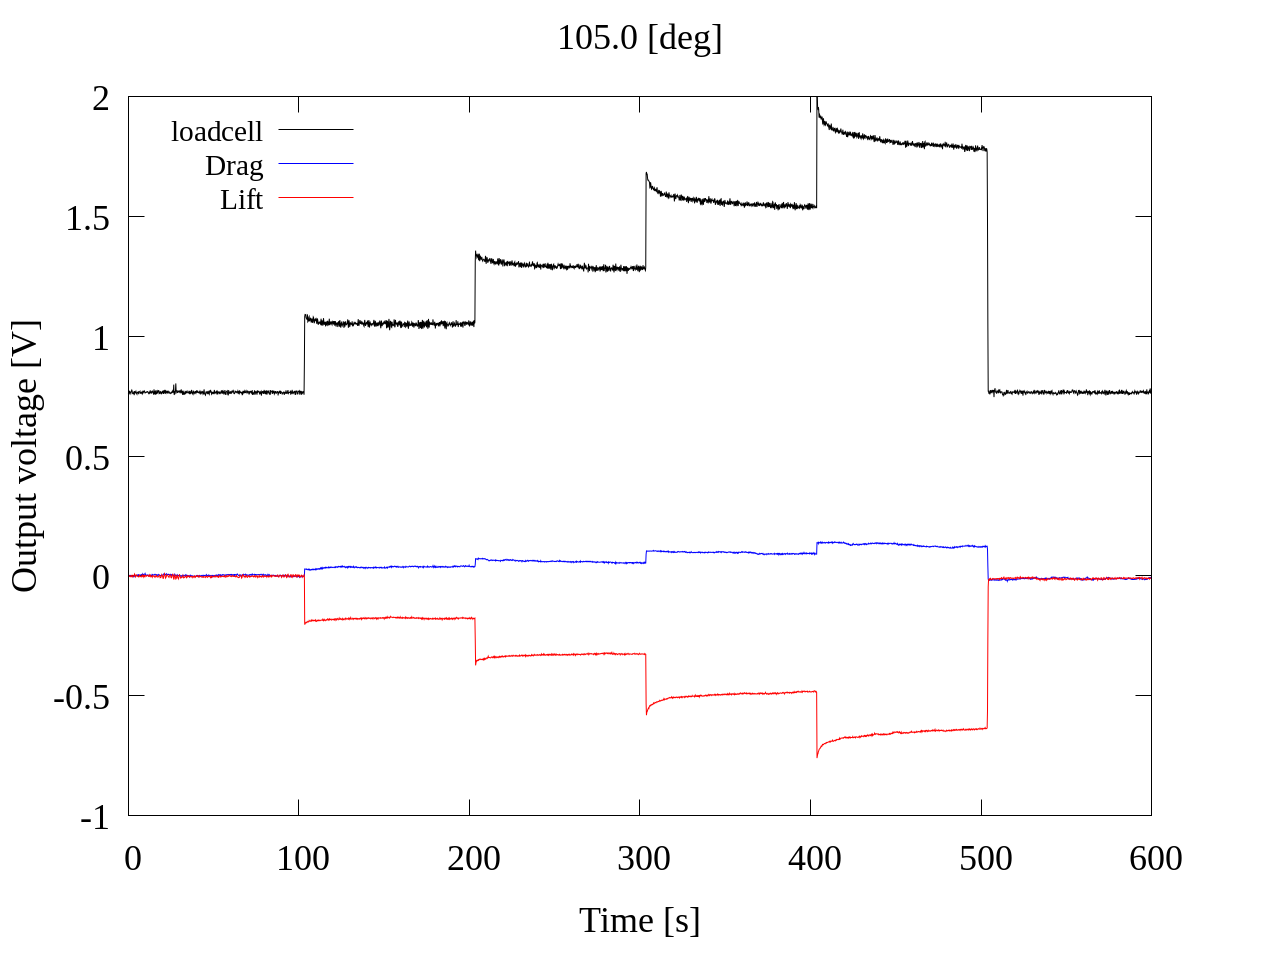
\includegraphics[width=65mm]{../../02_workspace/result/2-1/plot/01-3_allsensors/01_allsensors_1050.png}
        \caption{Output voltage : 105 [deg]}
      \end{minipage}\\
      \begin{minipage}[b]{0.45\linewidth}
        \centering
        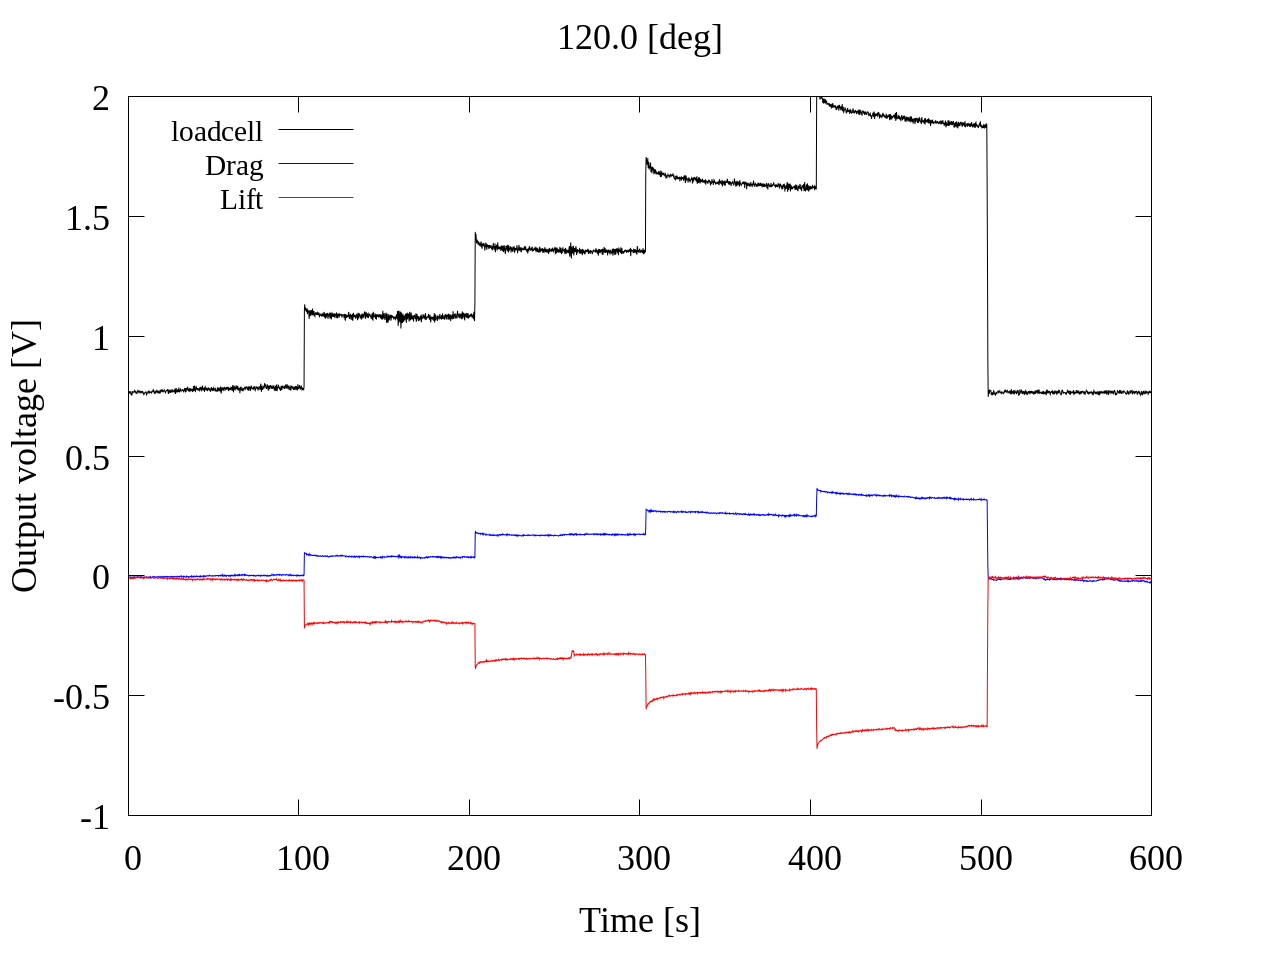
\includegraphics[width=65mm]{../../02_workspace/result/2-1/plot/01-3_allsensors/01_allsensors_1200.png}
        \caption{Output voltage : 120 [deg]}
      \end{minipage}
      \begin{minipage}[b]{0.45\linewidth}
        \centering
        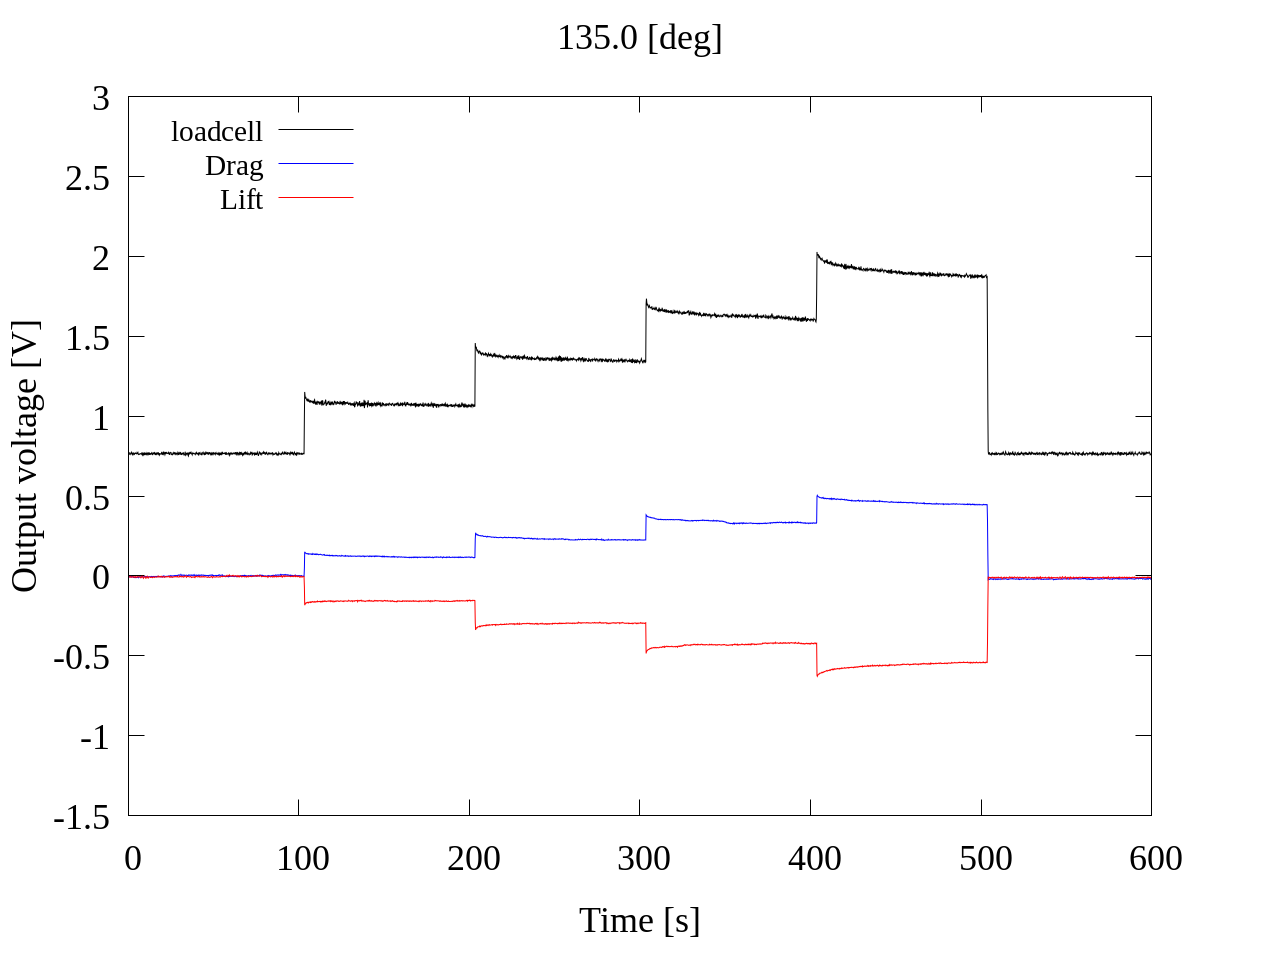
\includegraphics[width=65mm]{../../02_workspace/result/2-1/plot/01-3_allsensors/01_allsensors_1350.png}
        \caption{Output voltage : 135 [deg]}
      \end{minipage}\\
      \begin{minipage}[b]{0.45\linewidth}
        \centering
        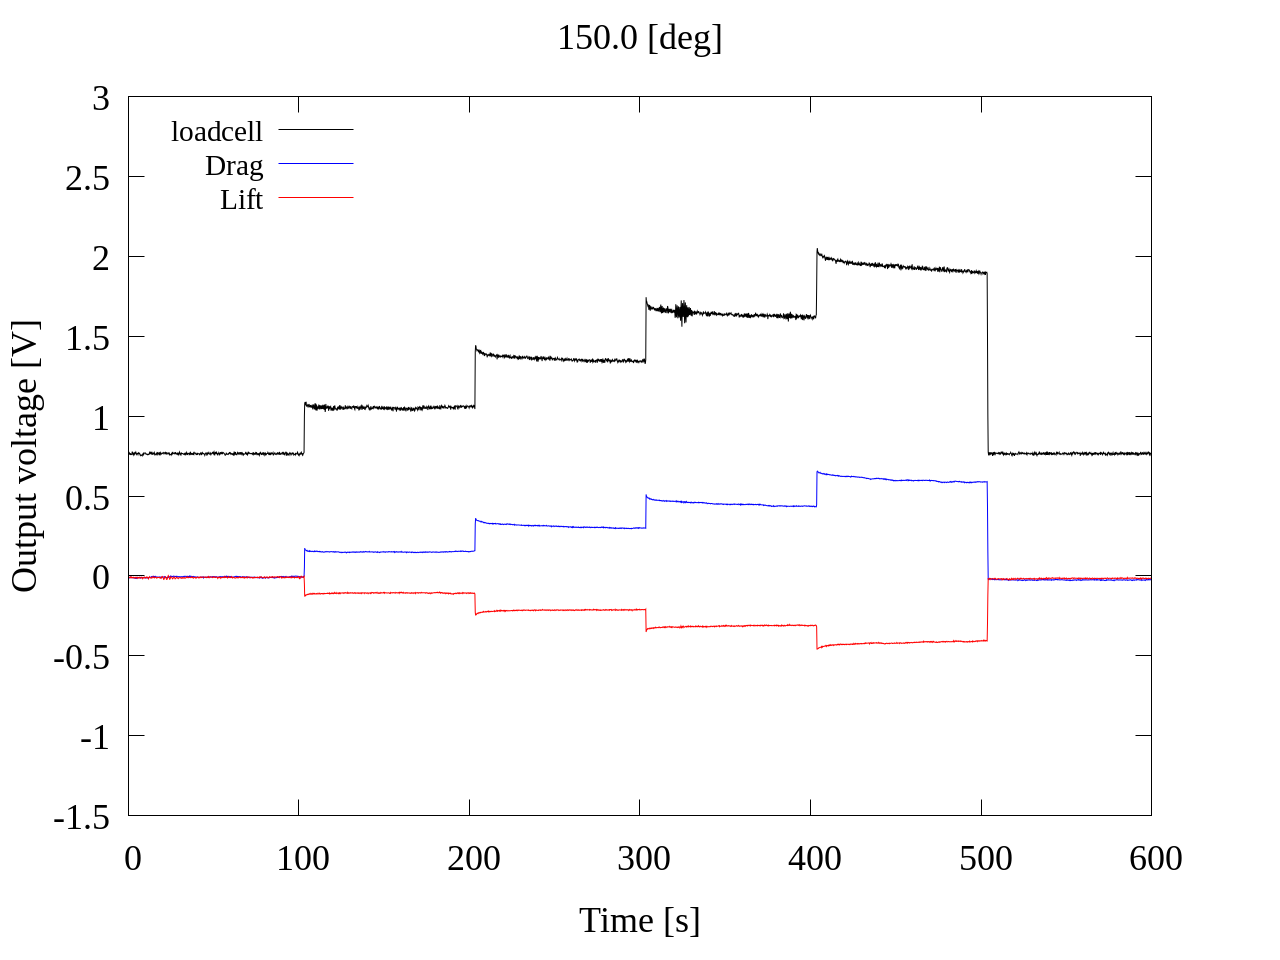
\includegraphics[width=65mm]{../../02_workspace/result/2-1/plot/01-3_allsensors/01_allsensors_1500.png}
        \caption{Output voltage : 150 [deg]}
      \end{minipage} 
      \begin{minipage}[b]{0.45\linewidth}
        \centering
        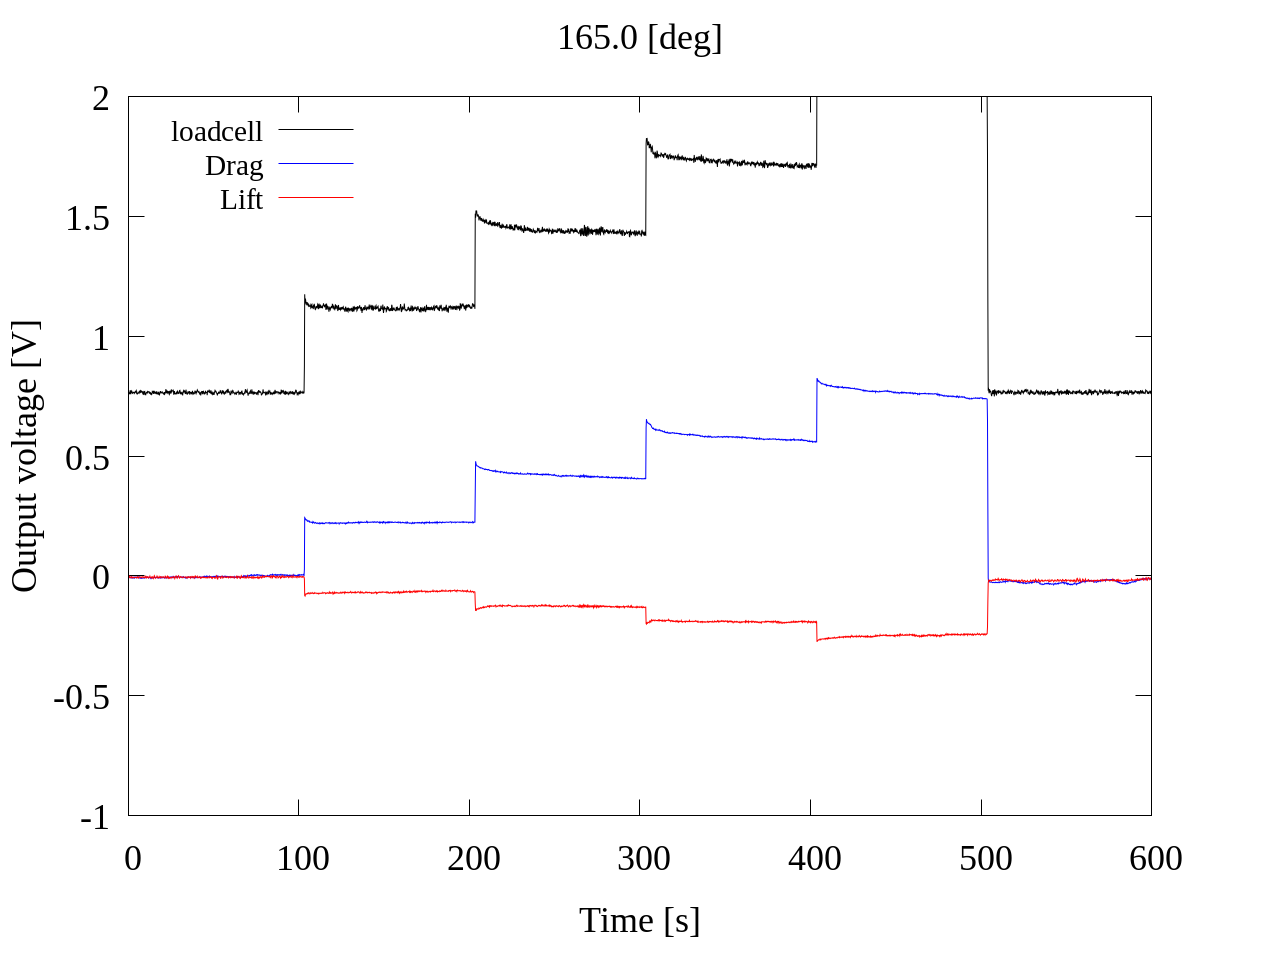
\includegraphics[width=65mm]{../../02_workspace/result/2-1/plot/01-3_allsensors/01_allsensors_1650.png}
        \caption{Output voltage : 165 [deg]}
      \end{minipage}\\
\end{figure}

\begin{figure}[htbp]
      \begin{minipage}[b]{0.45\linewidth}
        \centering
        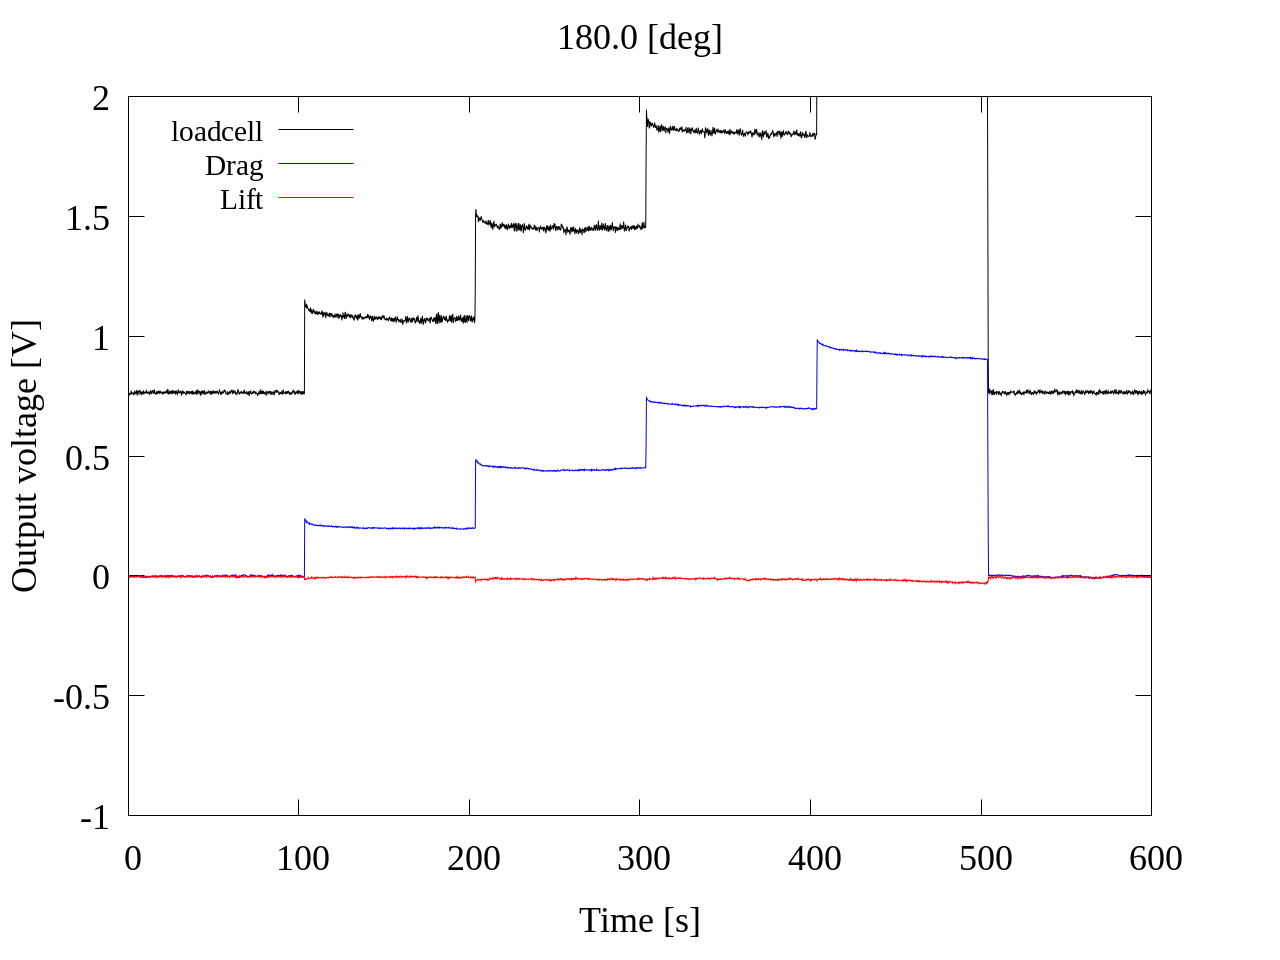
\includegraphics[width=65mm]{../../02_workspace/result/2-1/plot/01-3_allsensors/01_allsensors_1800.png}
        \caption{Output voltage : 180 [deg]}
      \end{minipage}
      \begin{minipage}[b]{0.45\linewidth}
        \centering
        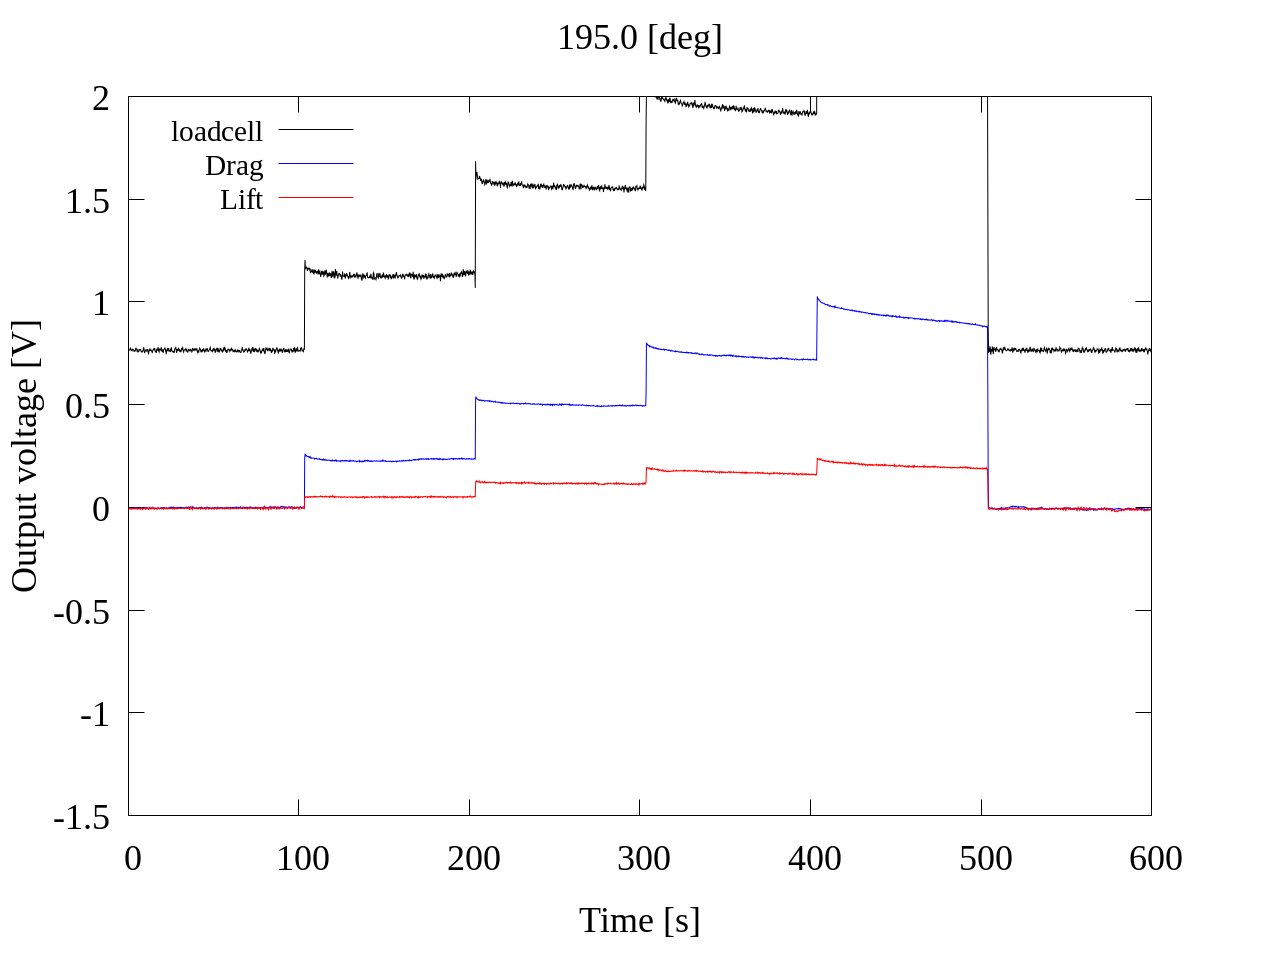
\includegraphics[width=65mm]{../../02_workspace/result/2-1/plot/01-3_allsensors/01_allsensors_1950.png}
        \caption{Output voltage : 195 [deg]}
      \end{minipage}\\

      \begin{minipage}[b]{0.45\linewidth}
        \centering
        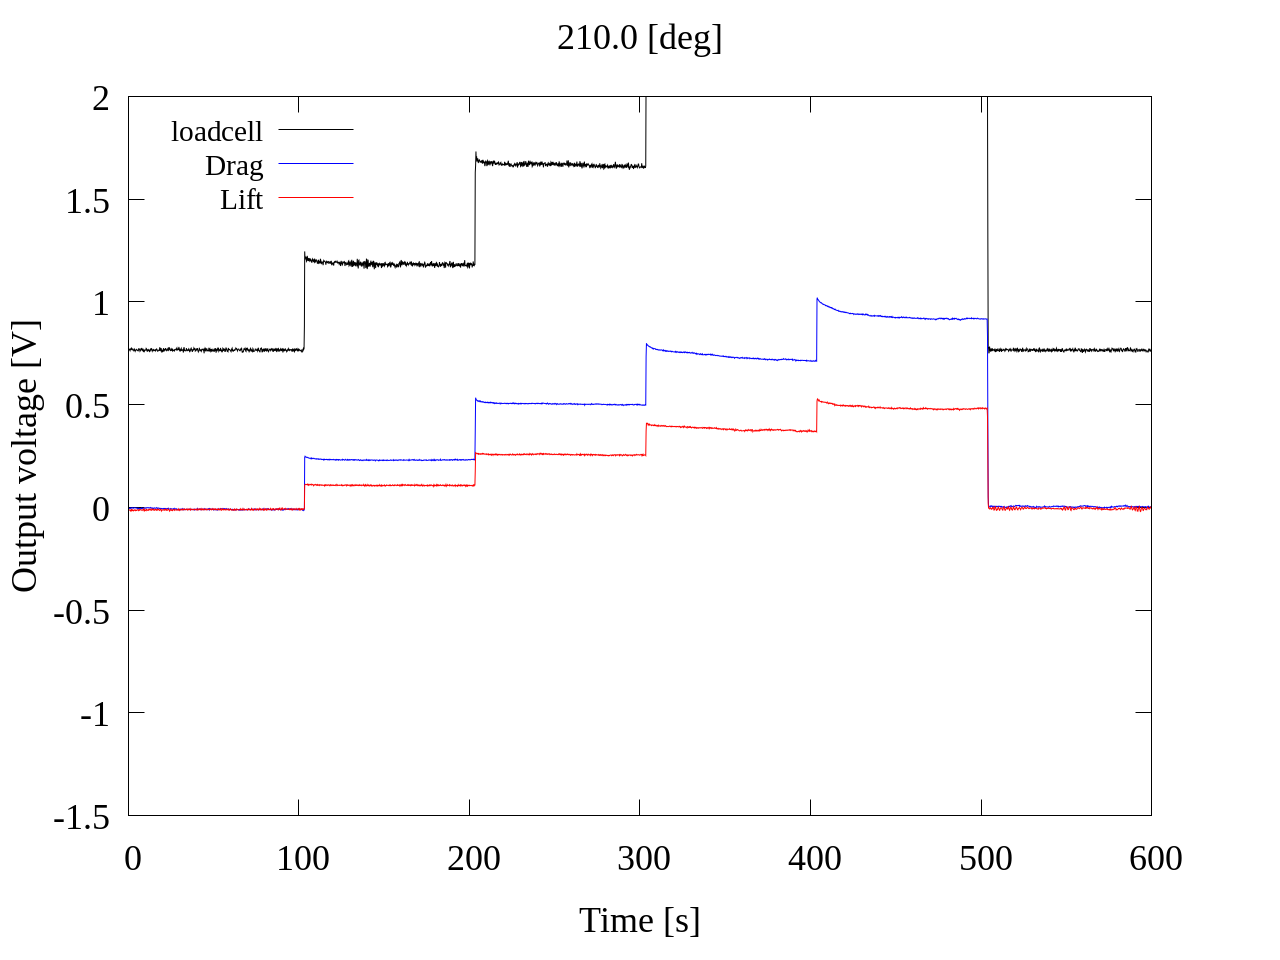
\includegraphics[width=65mm]{../../02_workspace/result/2-1/plot/01-3_allsensors/01_allsensors_2100.png}
        \caption{Output voltage : 210 [deg]}
      \end{minipage}
      \begin{minipage}[b]{0.45\linewidth}
        \centering
        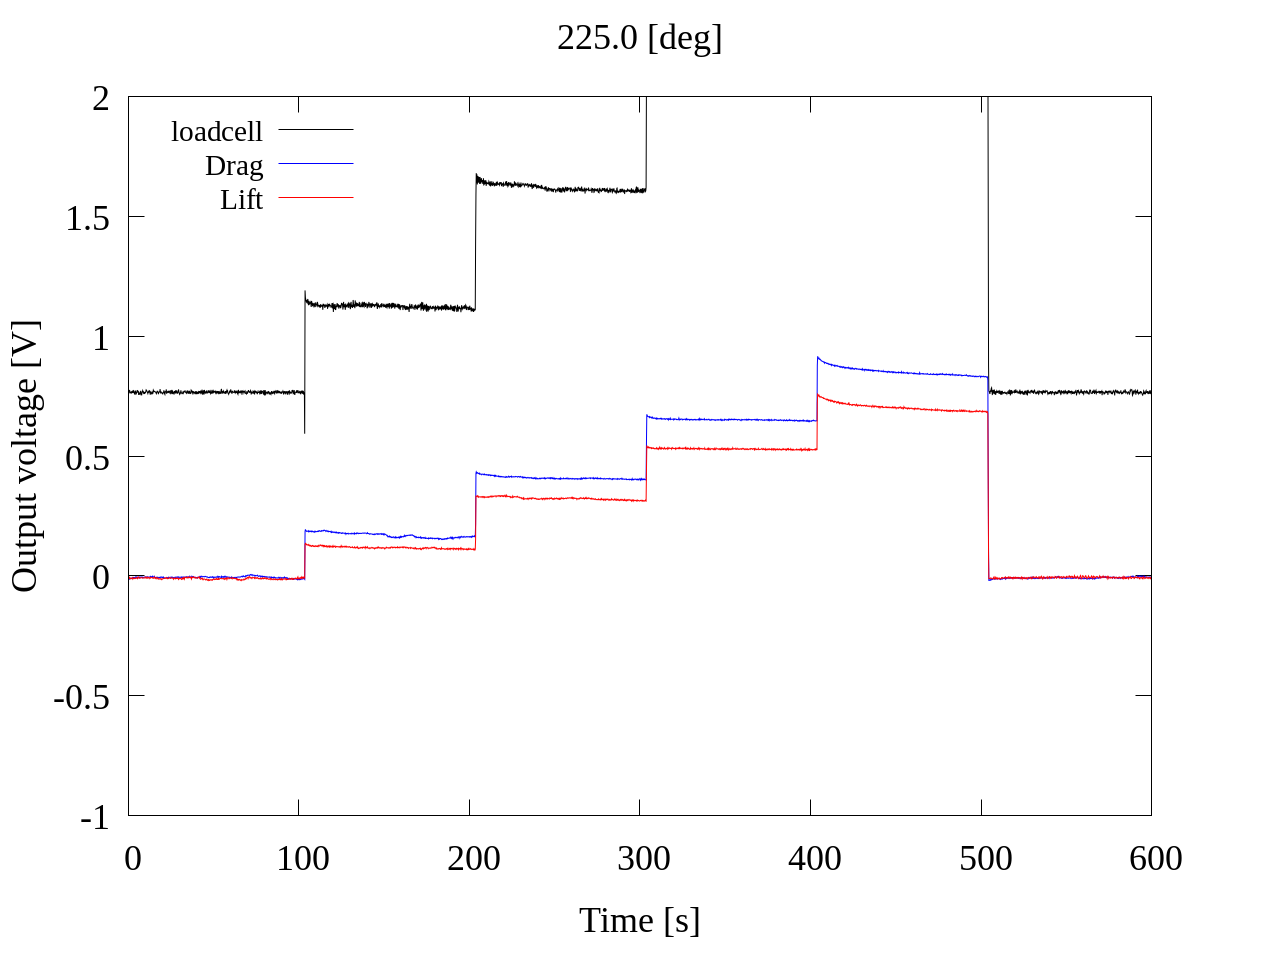
\includegraphics[width=65mm]{../../02_workspace/result/2-1/plot/01-3_allsensors/01_allsensors_2250.png}
        \caption{Output voltage : 225 [deg]}
      \end{minipage}\\

      \begin{minipage}[b]{0.45\linewidth}
        \centering
        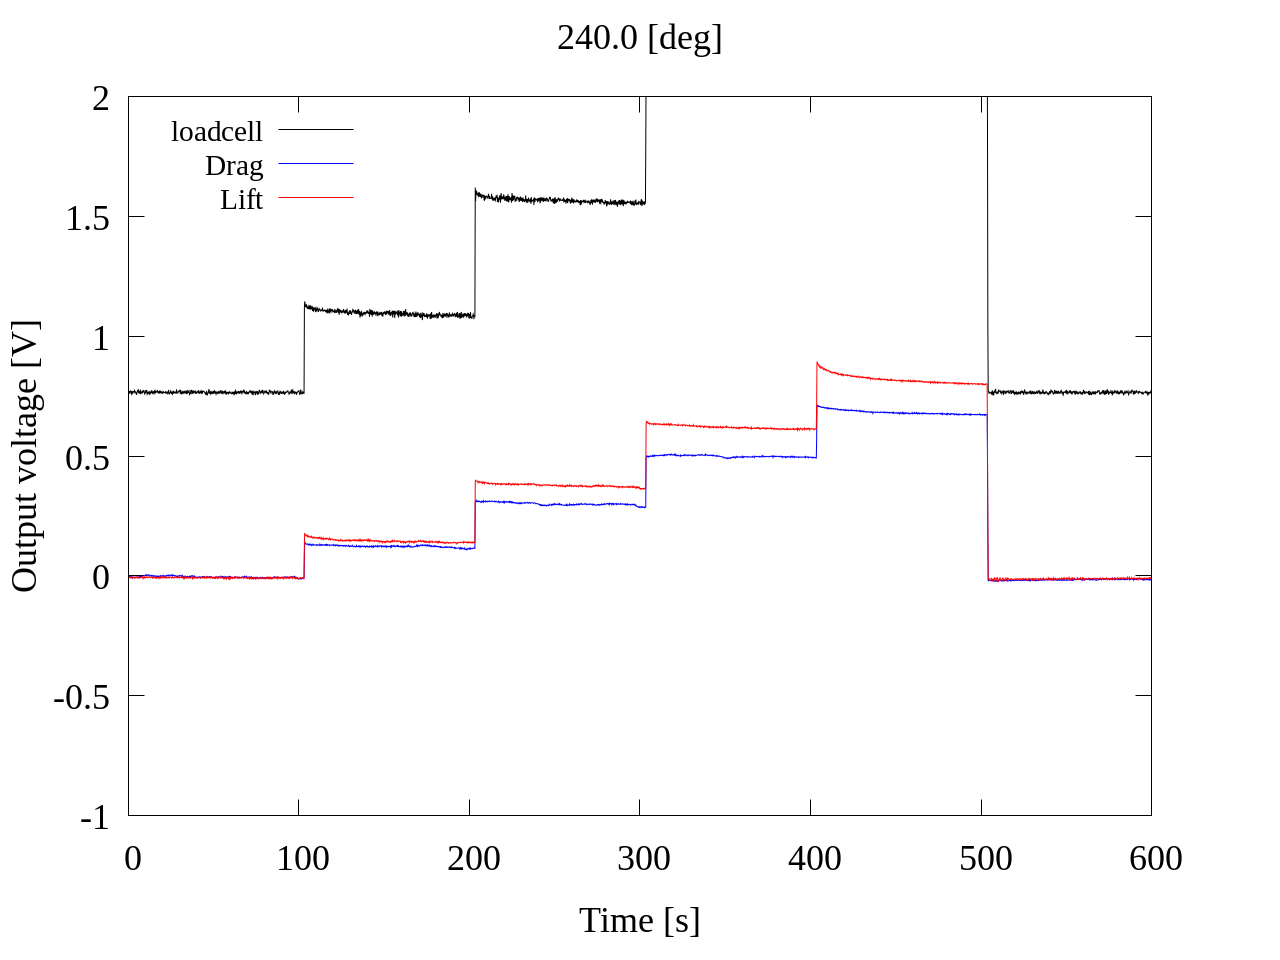
\includegraphics[width=65mm]{../../02_workspace/result/2-1/plot/01-3_allsensors/01_allsensors_2400.png}
        \caption{Output voltage : 240 [deg]}
      \end{minipage}
      \begin{minipage}[b]{0.45\linewidth}
        \centering
        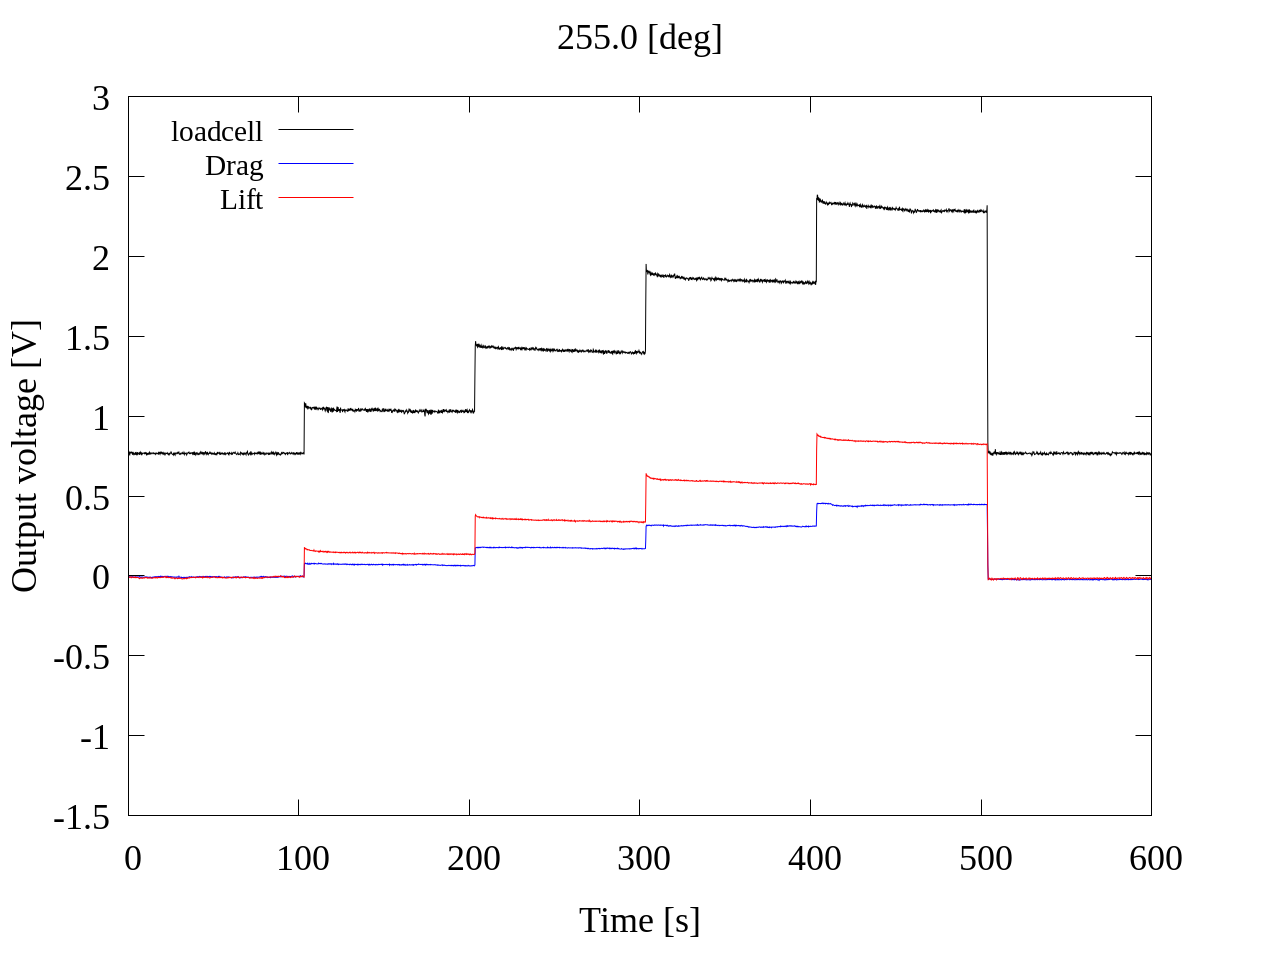
\includegraphics[width=65mm]{../../02_workspace/result/2-1/plot/01-3_allsensors/01_allsensors_2550.png}
        \caption{Output voltage : 255 [deg]}
      \end{minipage}
    \end{figure}

    \begin{figure}[htbp]
      \begin{minipage}[b]{0.45\linewidth}
        \centering
        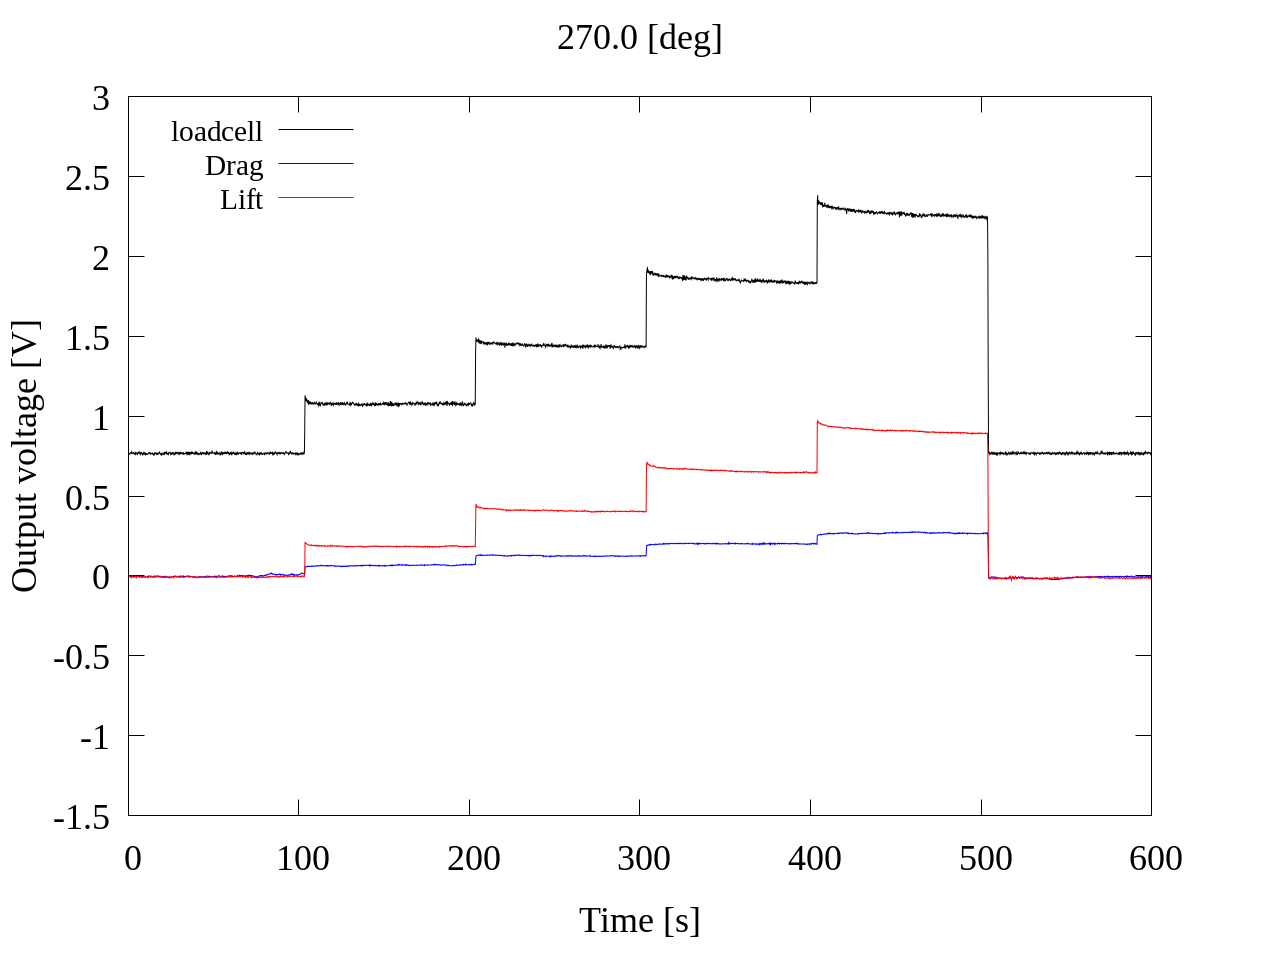
\includegraphics[width=65mm]{../../02_workspace/result/2-1/plot/01-3_allsensors/01_allsensors_2700.png}
        \caption{Output voltage : 270 [deg]}
      \end{minipage}
      \begin{minipage}[b]{0.45\linewidth}
        \centering
        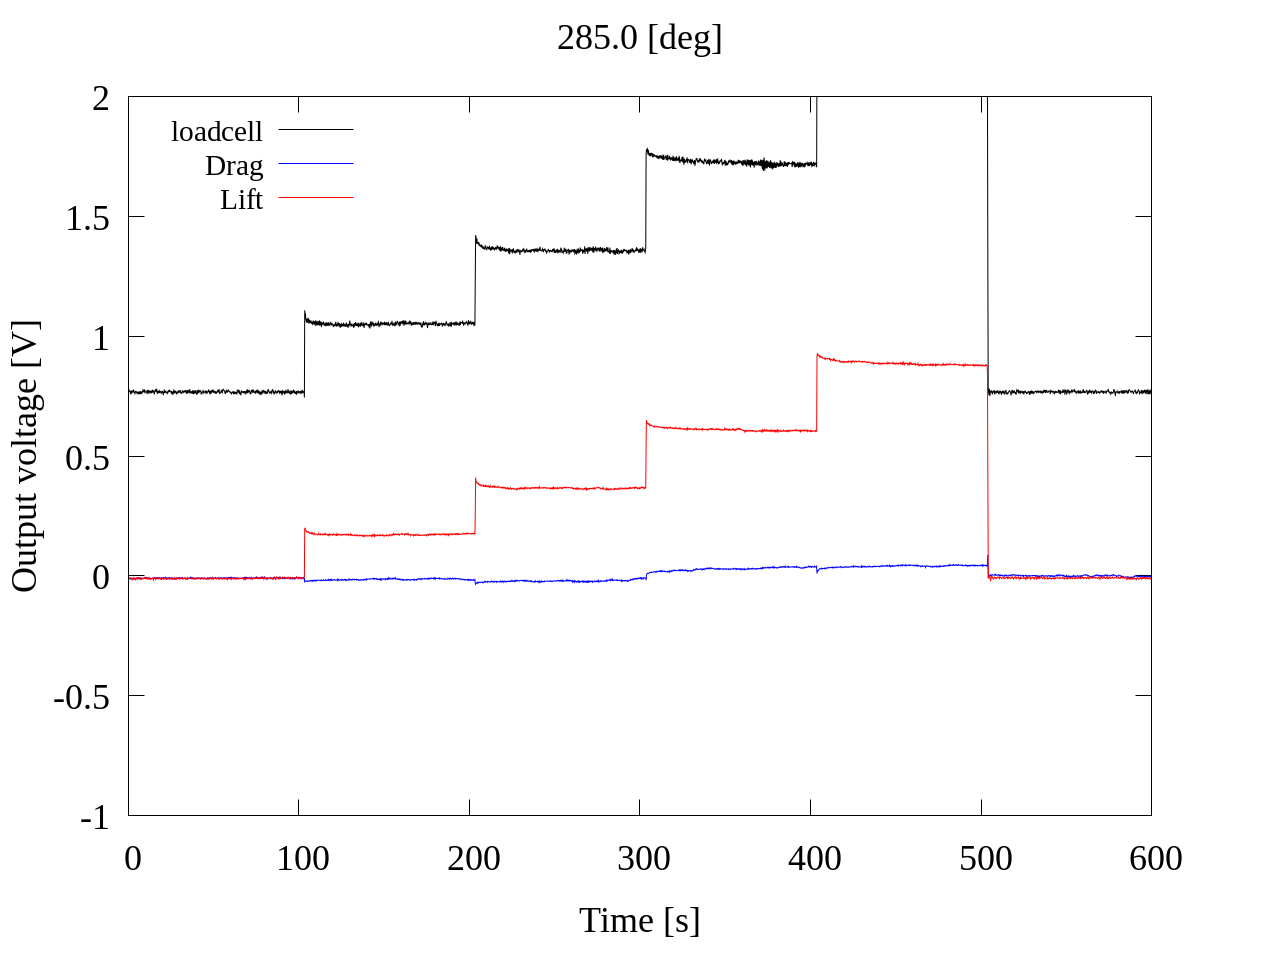
\includegraphics[width=65mm]{../../02_workspace/result/2-1/plot/01-3_allsensors/01_allsensors_2850.png}
        \caption{Output voltage : 285 [deg]}
      \end{minipage}\\

      \begin{minipage}[b]{0.45\linewidth}
        \centering
        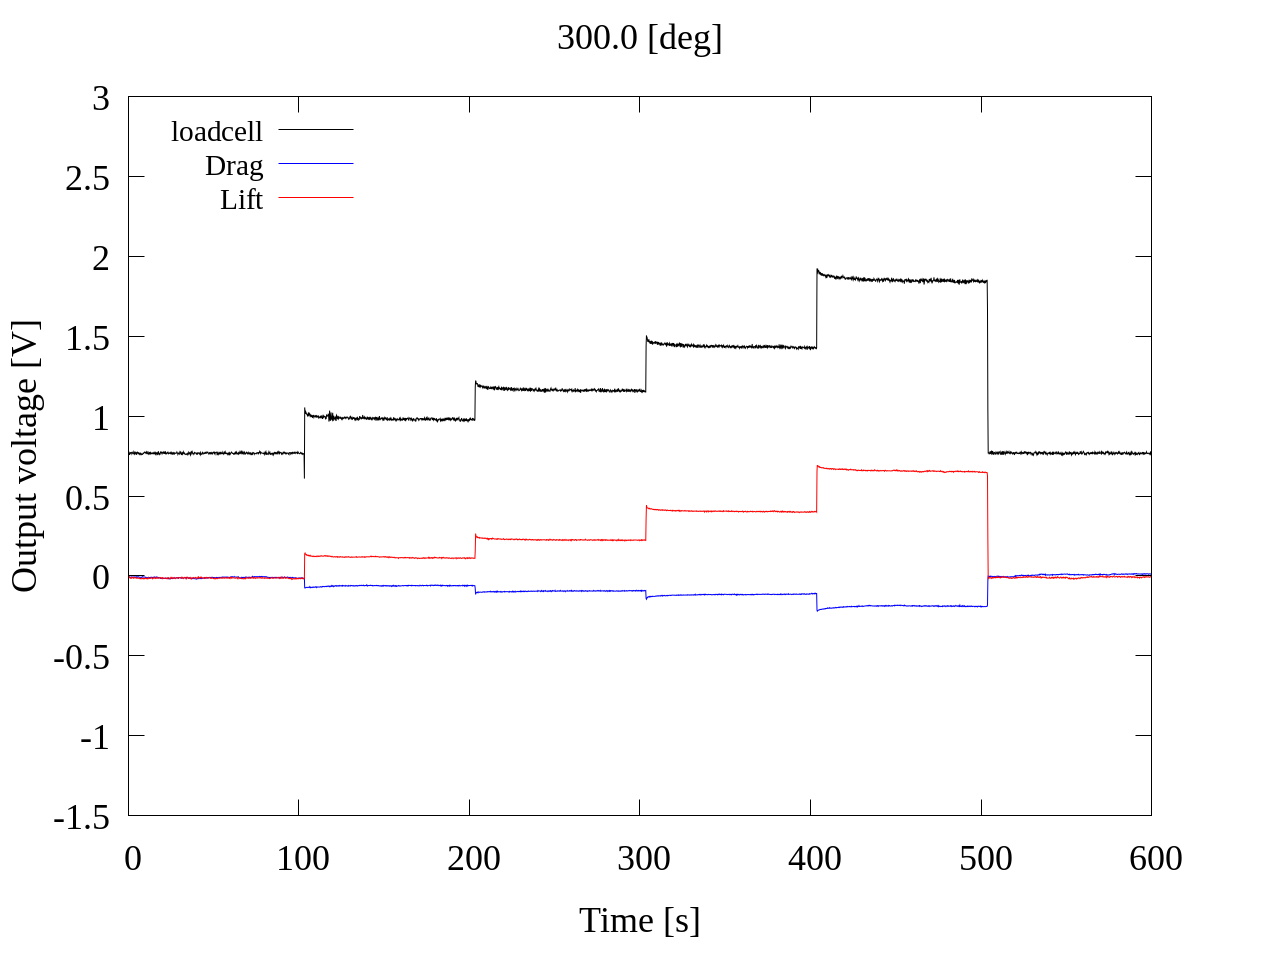
\includegraphics[width=65mm]{../../02_workspace/result/2-1/plot/01-3_allsensors/01_allsensors_3000.png}
        \caption{Output voltage : 300 [deg]}
      \end{minipage}
      \begin{minipage}[b]{0.45\linewidth}
        \centering
        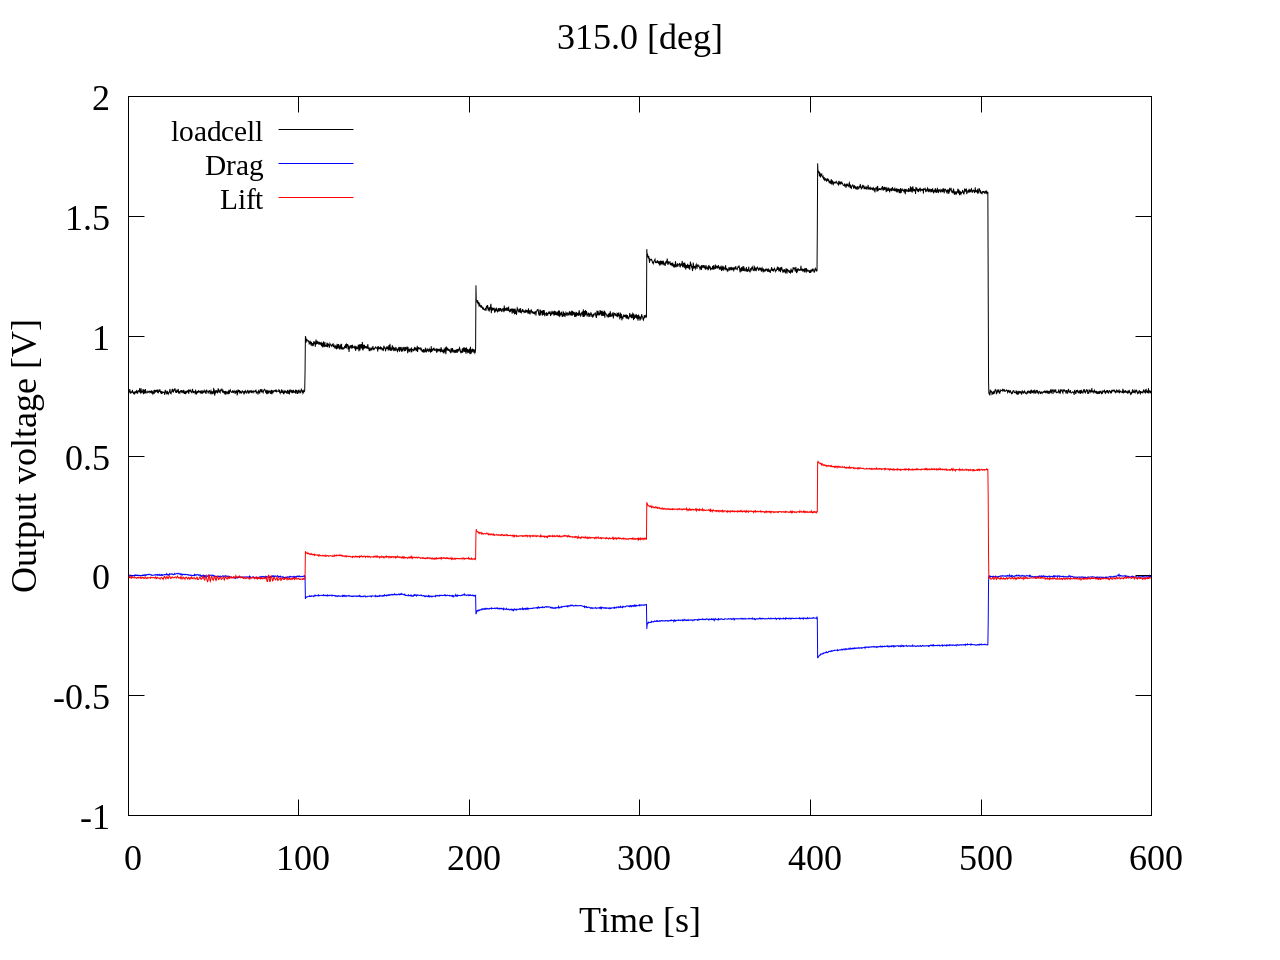
\includegraphics[width=65mm]{../../02_workspace/result/2-1/plot/01-3_allsensors/01_allsensors_3150.png}
        \caption{Output voltage : 315 [deg]}
      \end{minipage}\\

      \begin{minipage}[b]{0.45\linewidth}
        \centering
        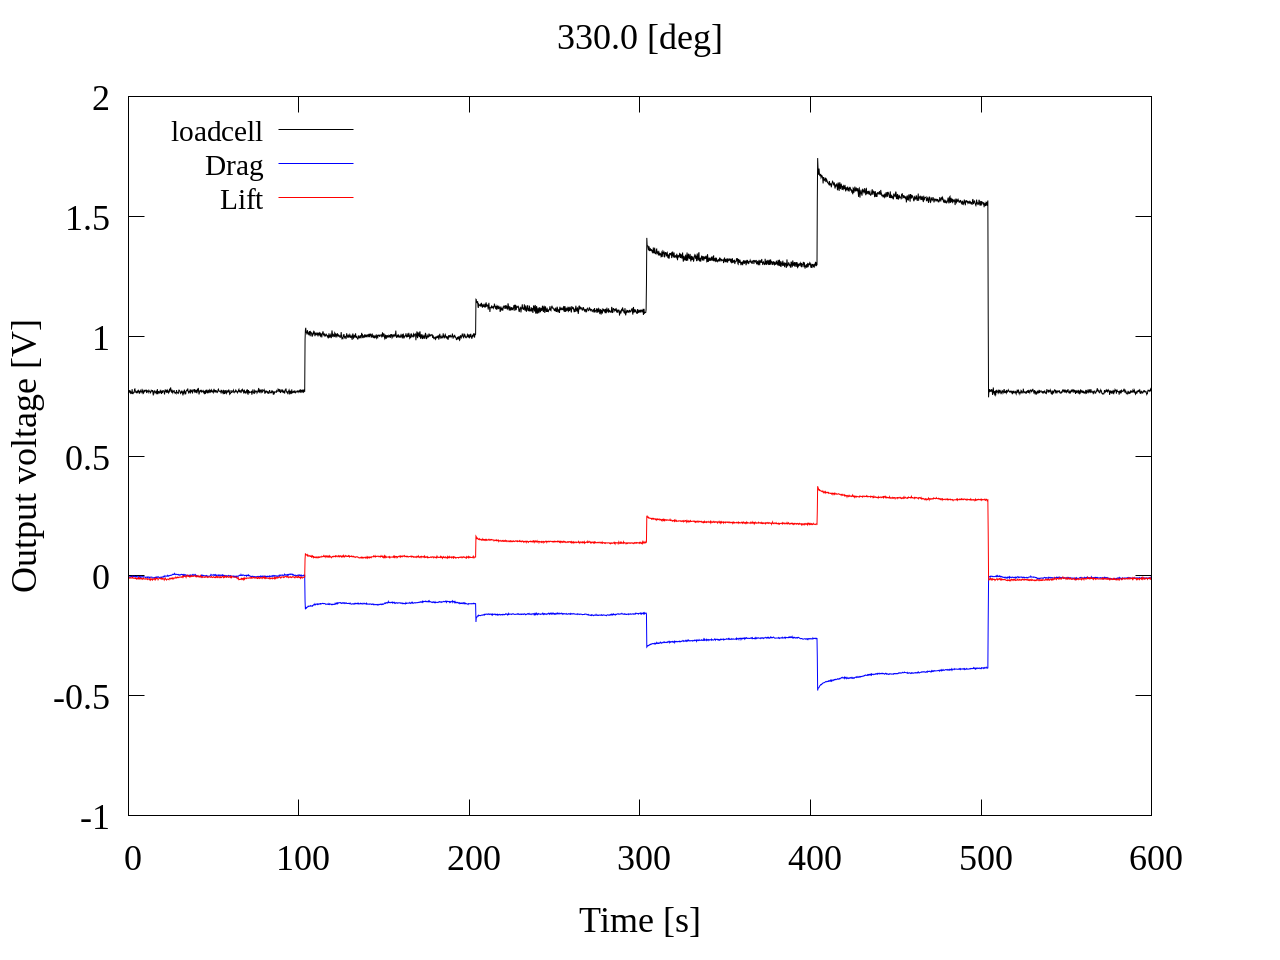
\includegraphics[width=65mm]{../../02_workspace/result/2-1/plot/01-3_allsensors/01_allsensors_3300.png}
        \caption{Output voltage : 330 [deg]}
      \end{minipage}
      \begin{minipage}[b]{0.45\linewidth}
        \centering
        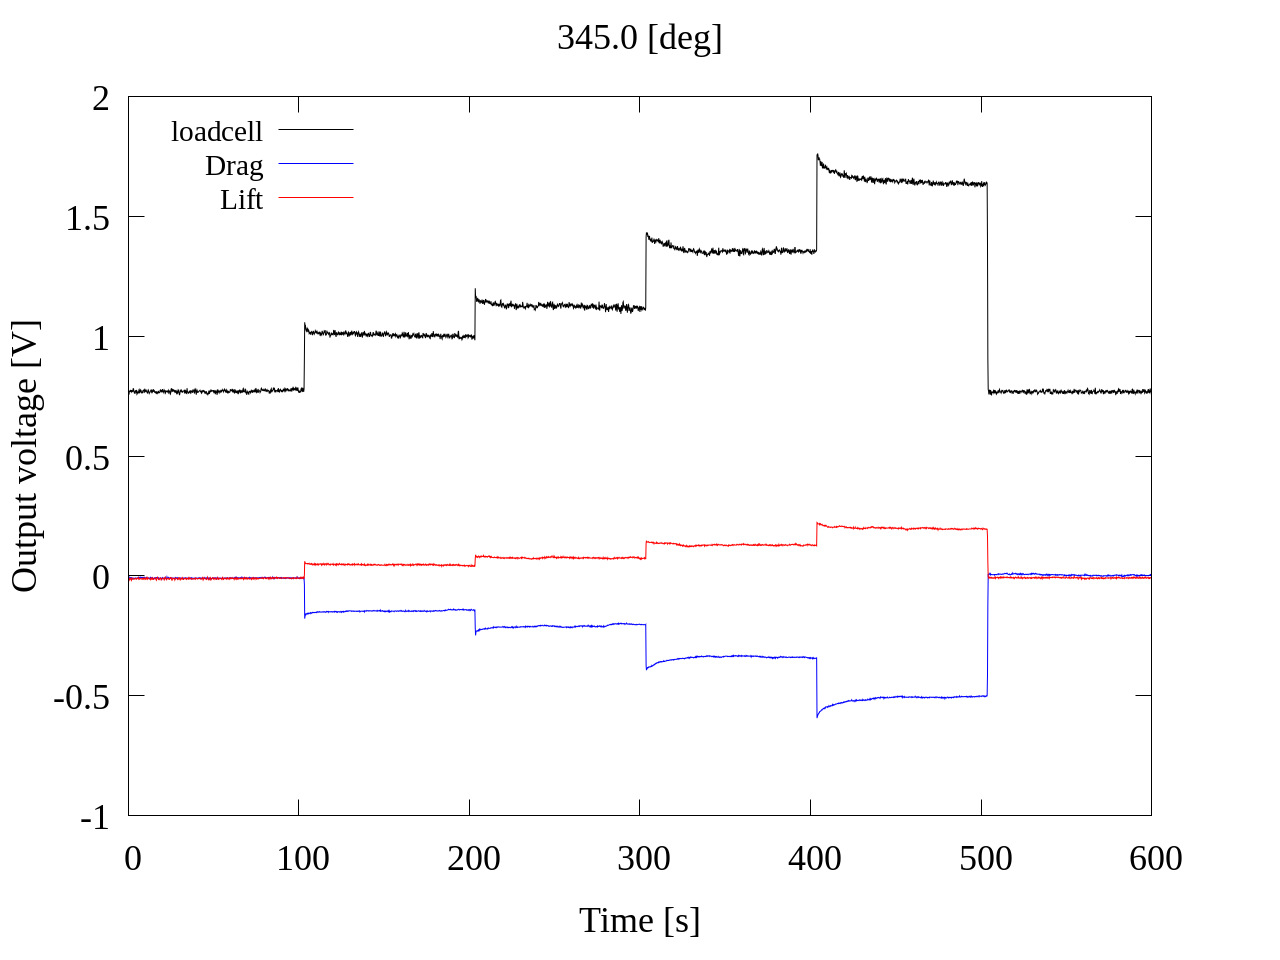
\includegraphics[width=65mm]{../../02_workspace/result/2-1/plot/01-3_allsensors/01_allsensors_3450.png}
        \caption{Output voltage : 345 [deg]}
      \end{minipage}
\end{figure}

\newpage

以上の結果から自動一軸ステージが移動した直後から出力電圧の減衰がみられる場合があるが,
同様の変化がロードセルおよびひずみセンサにみられることから大きな問題はないと考える.

\subsection{データ処理手法}

実験結果から,式()の出力電圧勾配を算出する.
そのために以下の手順でデータ処理を行った.

\begin{enumerate}[2.3.1]
	\item ドリフト補正
	\item 各距離における平均値の算出
	\item 出力電圧勾配の算出
\end{enumerate}

ここで,例として 1回目の性能評価実験,0 [deg]におけるロードセルの出力電圧の図 (Fig.) を用いて説明する.\\

\begin{figure}[htbp]
	\footnotesize
	\begin{center}
		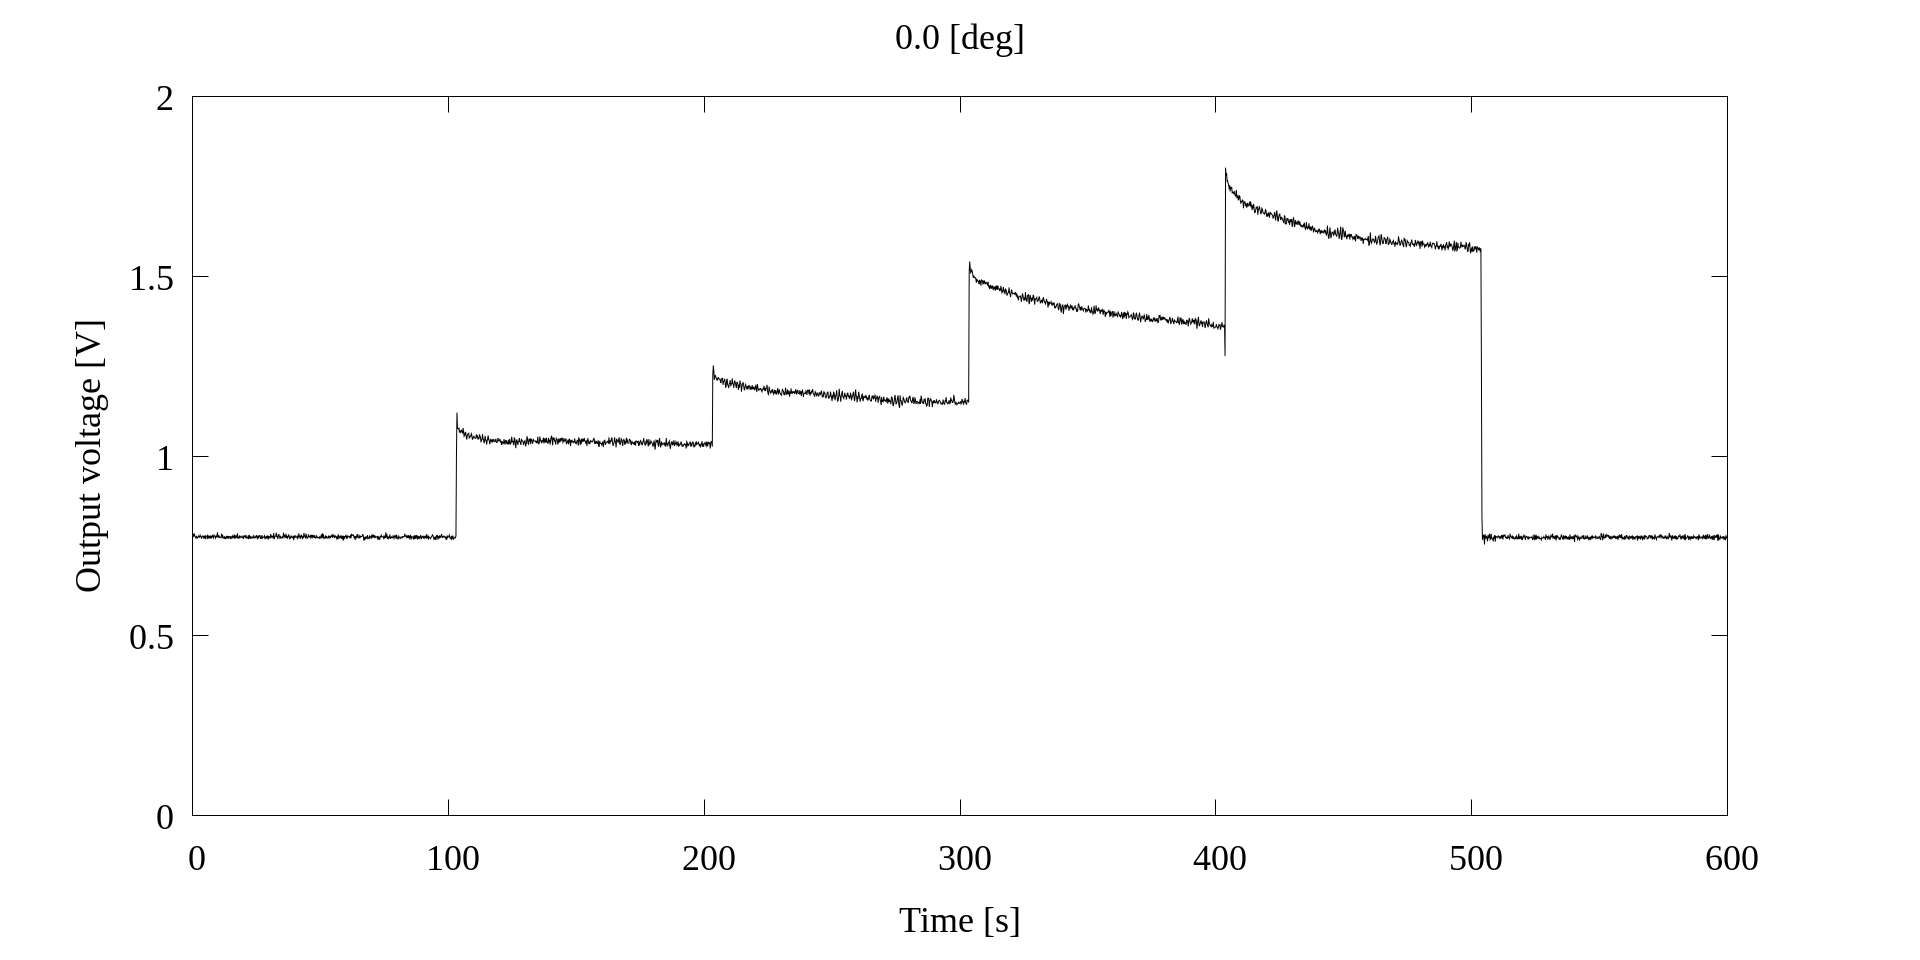
\includegraphics[width=95mm]{../../02_workspace/result/2-1/plot/01-1_loadcell/01_loadcell_0.png}
		\caption{Loadcell output voltage : 0 [deg] (1st)}
	\end{center}
\end{figure}

※ ロードセルの出力電圧は使用しているストレインアンプの影響によりオフセット値を持つ.

また,このとき実験結果をロードセルの押込距離および時間経過によって
それぞれのデータ範囲についてその呼称を以下のTable のように定義することとする.

\begin{table}[htbp]
	\begin{center}
		\caption{Definition of data name}
		\begin{tabular}{|p{20mm}|p{20mm}|p{20mm}|}
			\hline
			\multicolumn{1}{|c|}{\textgt{Data name}} & \multicolumn{1}{|c|}{\textgt{Pushing length [mm]}} & \multicolumn{1}{|c|}{\textgt{Time [s]}} \\ \hline
			\multicolumn{1}{|c|}{Range : 1}          & \multicolumn{1}{|c|}{0.00}                         & \multicolumn{1}{|c|}{0 $\sim$ 100}      \\ \hline
			\multicolumn{1}{|c|}{Range : 2}          & \multicolumn{1}{|c|}{0.03}                         & \multicolumn{1}{|c|}{100 $\sim$ 200}    \\ \hline
			\multicolumn{1}{|c|}{Range : 3}          & \multicolumn{1}{|c|}{0.06}                         & \multicolumn{1}{|c|}{200 $\sim$ 300}    \\ \hline
			\multicolumn{1}{|c|}{Range : 4}          & \multicolumn{1}{|c|}{0.09}                         & \multicolumn{1}{|c|}{300 $\sim$ 400}    \\ \hline
			\multicolumn{1}{|c|}{Range : 5}          & \multicolumn{1}{|c|}{0.12}                         & \multicolumn{1}{|c|}{400 $\sim$ 500}    \\ \hline
			\multicolumn{1}{|c|}{Range : 6}          & \multicolumn{1}{|c|}{0.00}                         & \multicolumn{1}{|c|}{500 $\sim$ 600}    \\ \hline
		\end{tabular}
	\end{center}
\end{table}

\newpage

\subsubsection{ドリフト補正}
性能評価実験は各角度に対して約10分間の測定を行うが,
ストレインアンプは時間経過に対して基準の電圧が変動する場合がある.
この現象をドリフトと呼ぶ.
そのため,実験結果を出力電圧勾配の算出に用いる
前処理として,ドリフトを考慮したデータへと変換する必要がある.

このとき,以下の手順でドリフト補正を行うこととする.

\begin{enumerate}[(1)]
	\item 測定開始直後(Range : 1)及び終了直前(Range : 6)のデータ(30秒/150点)における平均値を算出
	\item 算出した2つの平均値を結び,直線を作成
	\item 元データと直線の差をとり,補正値として採用する
\end{enumerate}

以下のFig. にドリフト補正を適用した結果を示す.

\begin{figure}[htbp]
	\footnotesize
	\begin{center}
		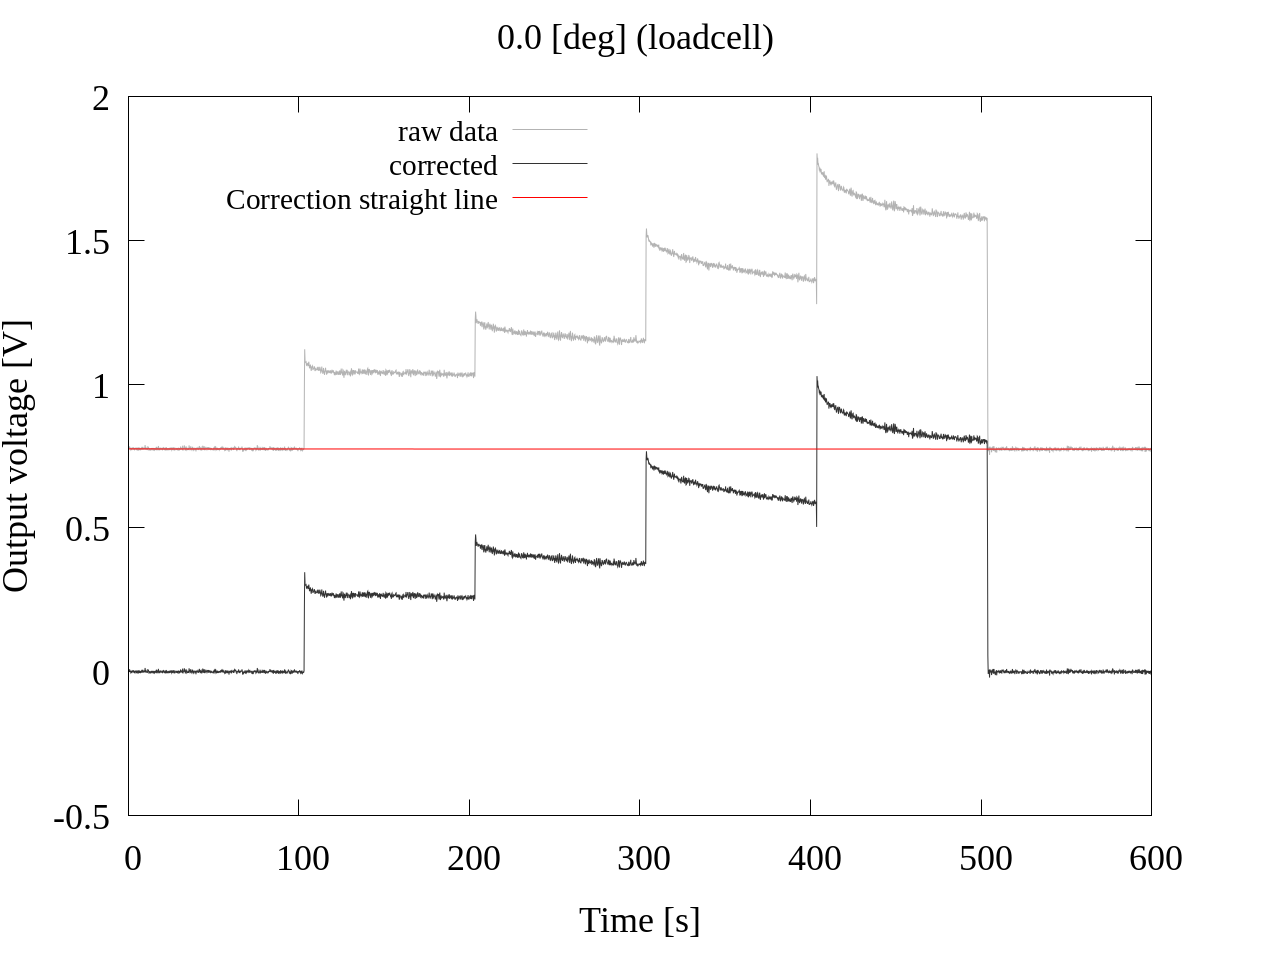
\includegraphics[width=95mm]{../../02_workspace/result/2-1/plot/02-1_loadcell/02_loadcell-drift_0.png}
		\caption{Drift corrected (load cell) : 0 [deg] (1st)}
	\end{center}
\end{figure}

Fig.から補正前のデータから算出された補正直線(赤線)の差を取ると
補正後のデータはオフセット値の分だけ移動しており,
タイヤモデルと接触していないとき($t = 0 \sim 100 \; [\mathrm{s}]$,$t = 500 \sim 600 \; [\mathrm{s}]$)の
出力電圧の値は0付近を推移していることがわかる.
したがって,ドリフト補正処理は正しく動作していると考えられる.

また,以下のFig.に抗力及び揚力方向のひずみセンサの出力電圧について
同様のプログラムを用いてドリフト補正処理を行った結果を示す.

\begin{figure}[htbp]
	\footnotesize
	\begin{center}
		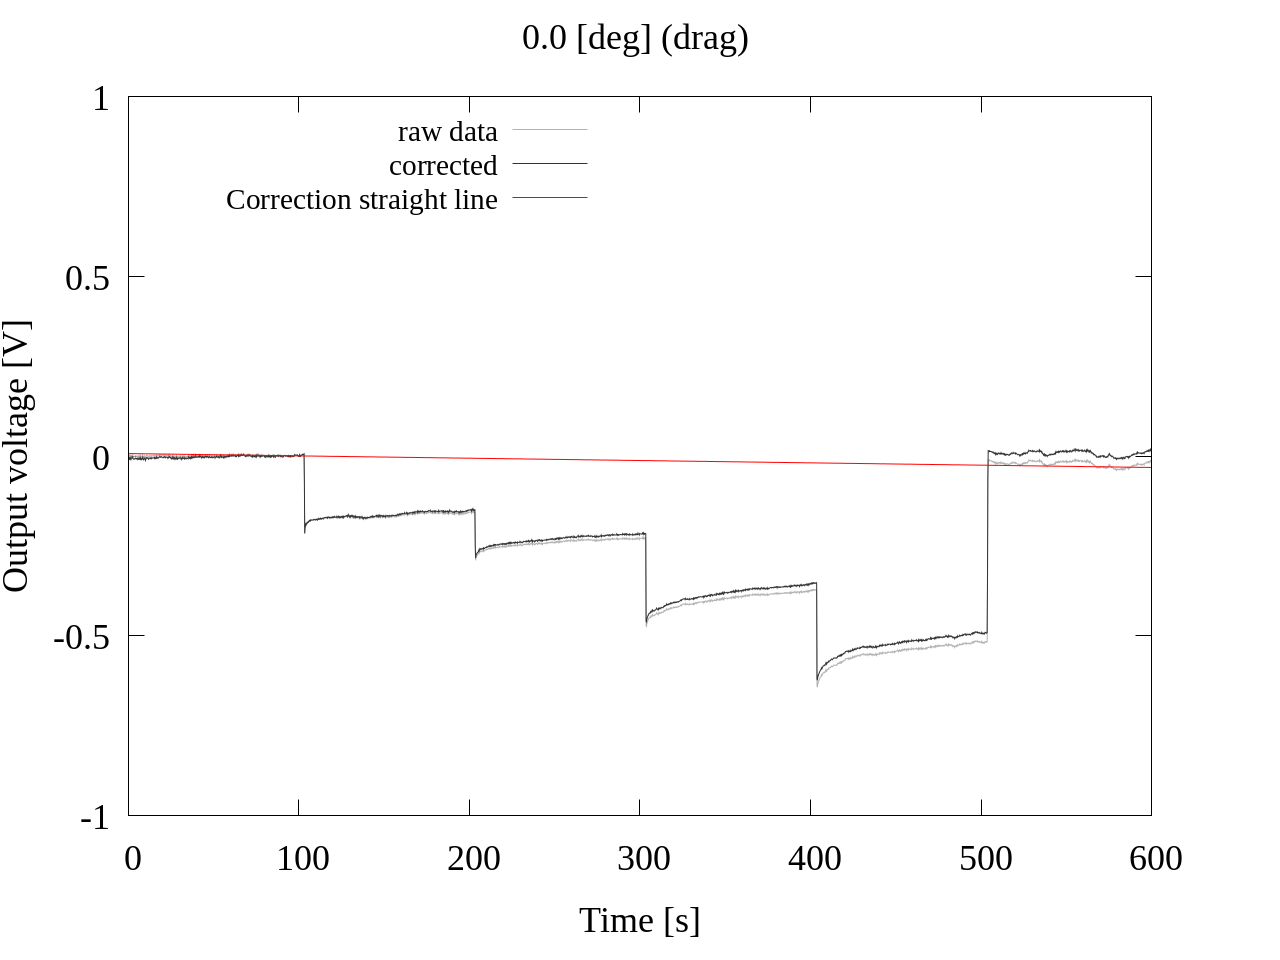
\includegraphics[width=95mm]{../../02_workspace/result/2-1/plot/02-2_drag/02_drag-drift_0.png}
		\caption{Drift corrected (drag) : 0 [deg] (1st)}
		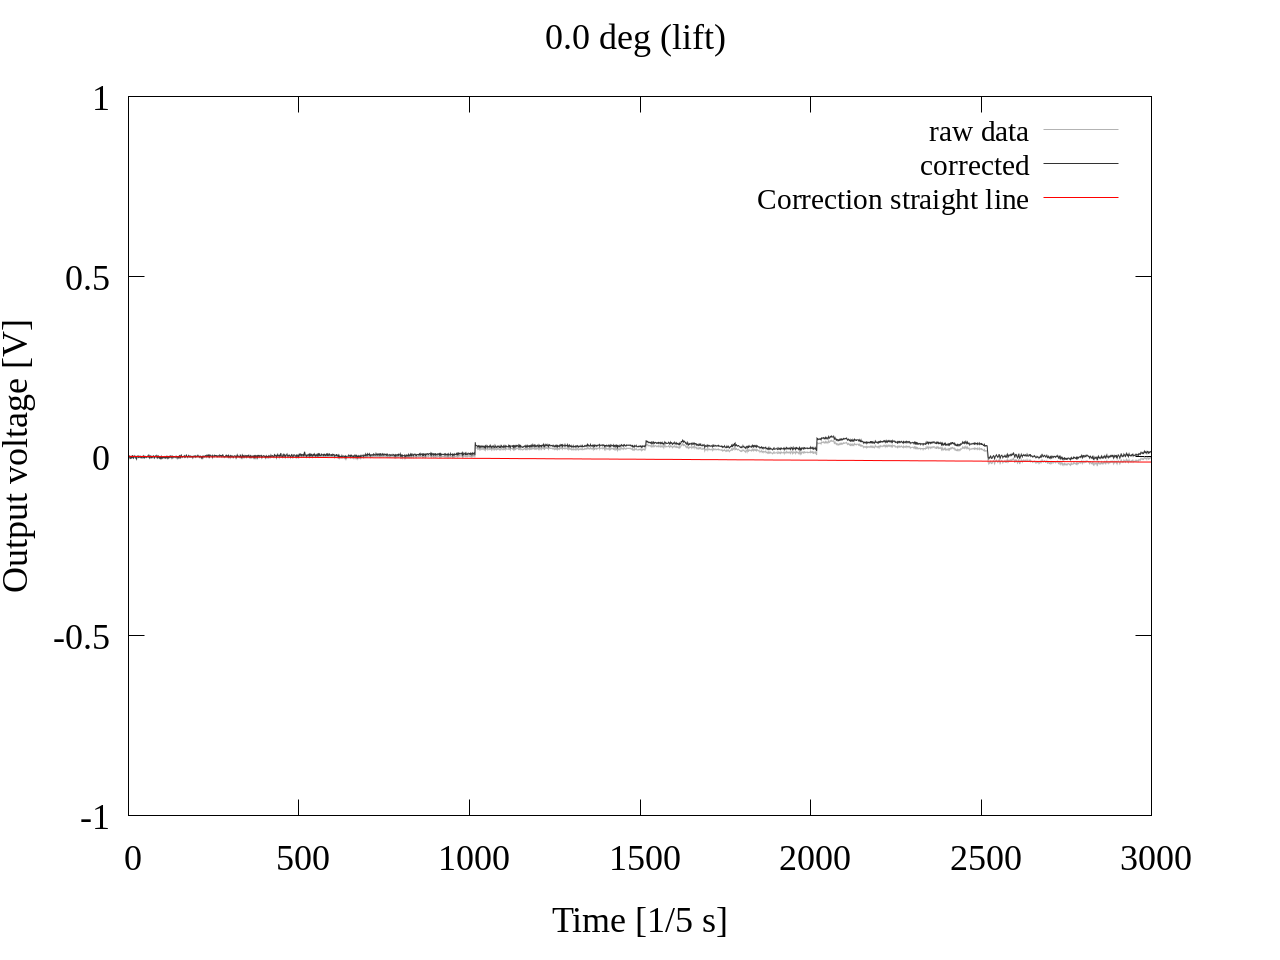
\includegraphics[width=95mm]{../../02_workspace/result/2-1/plot/02-3_lift/02_lift-drift_0.png}
		\caption{Drift corrected (lift) : 0 [deg] (1st)}
	\end{center}
\end{figure}

\newpage

\subsubsection{各距離における平均値の算出}

測定データの時間経過に沿って,プログラムの適用範囲を定め,
以下の手順からそれぞれのデータ範囲における出力電圧について平均値を算出した.

\begin{enumerate}[(1)]
	\item 各押込距離において測定した40秒間(計200点)のデータを使用
	\item 前後5秒(各25点)のデータを除いた30秒間(計150点)のデータの平均値を算出する
\end{enumerate}

以下のFig. にロードセルの出力電圧について平均値を算出した結果を示す.

\begin{figure}[htbp]
	\footnotesize
	\begin{center}
		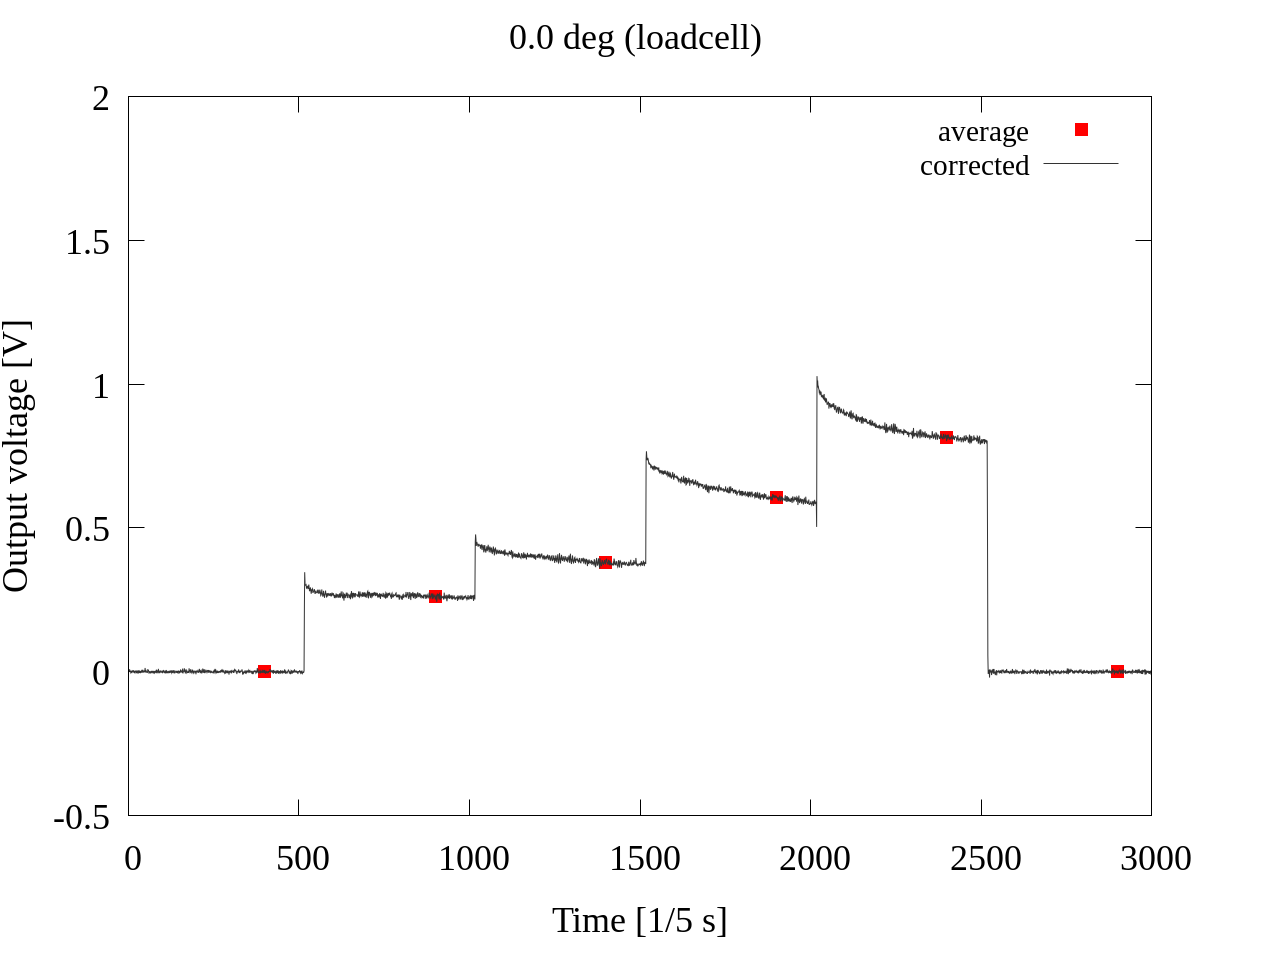
\includegraphics[width=95mm]{../../02_workspace/result/2-1/plot/03-1_loadcell/03_loadcell_average_0.png}
		\caption{Each distance average (load cell) : 0 [deg] (1st)}
	\end{center}
\end{figure}

また,以下のFig.に抗力及び揚力方向のひずみセンサの出力電圧について
同様のプログラムを用いて平均値の算出を行った結果を示す.

\begin{figure}[htbp]
	\begin{minipage}[b]{0.45\linewidth}
		\centering
		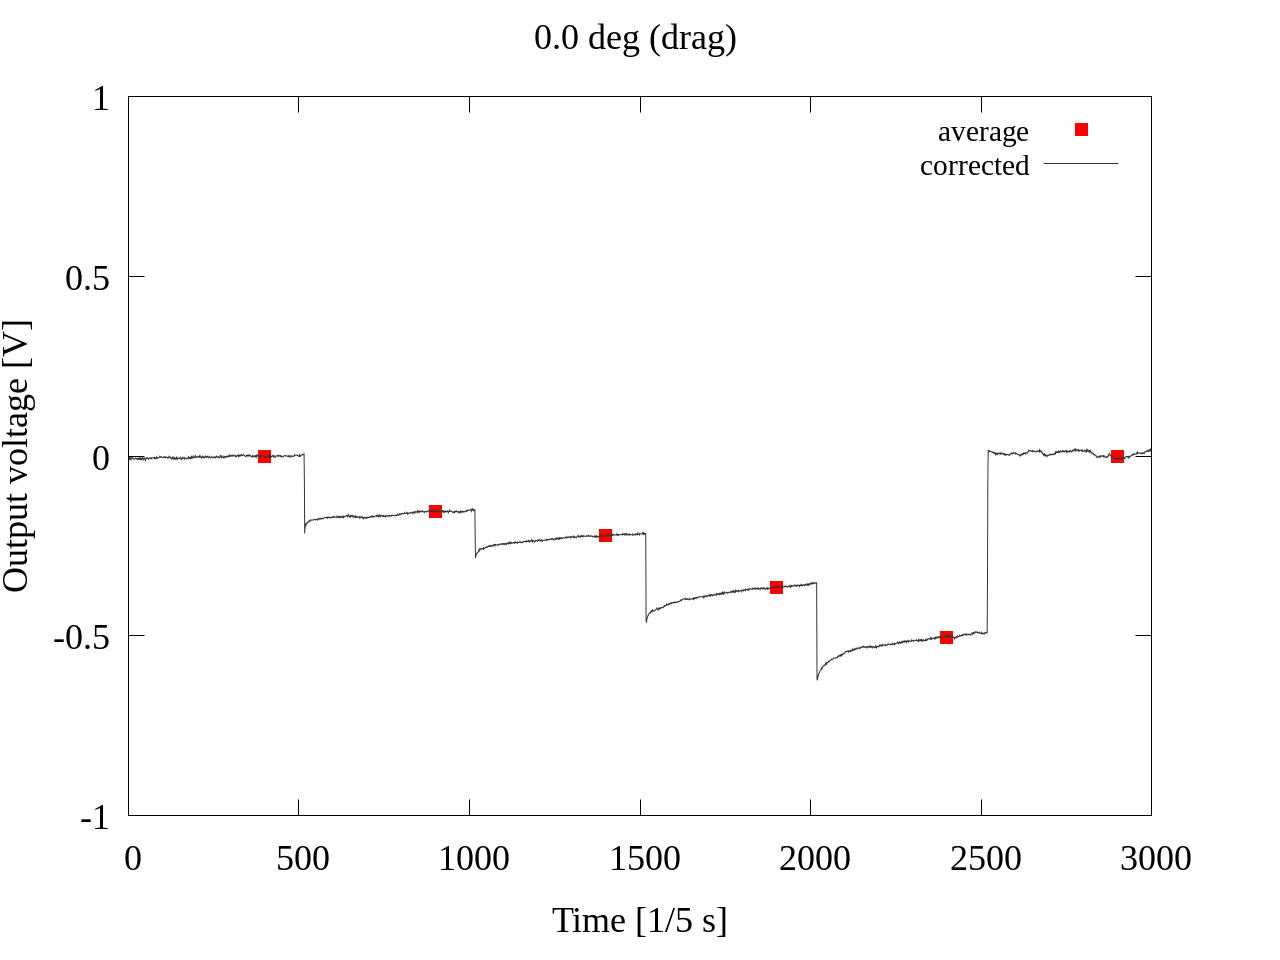
\includegraphics[width=65mm]{../../02_workspace/result/2-1/plot/03-2_drag/03_drag_average_0.png}
		\caption{Drift corrected (drag) : 0 [deg] (1st)}
	\end{minipage}
	\begin{minipage}[b]{0.45\linewidth}
		\centering
		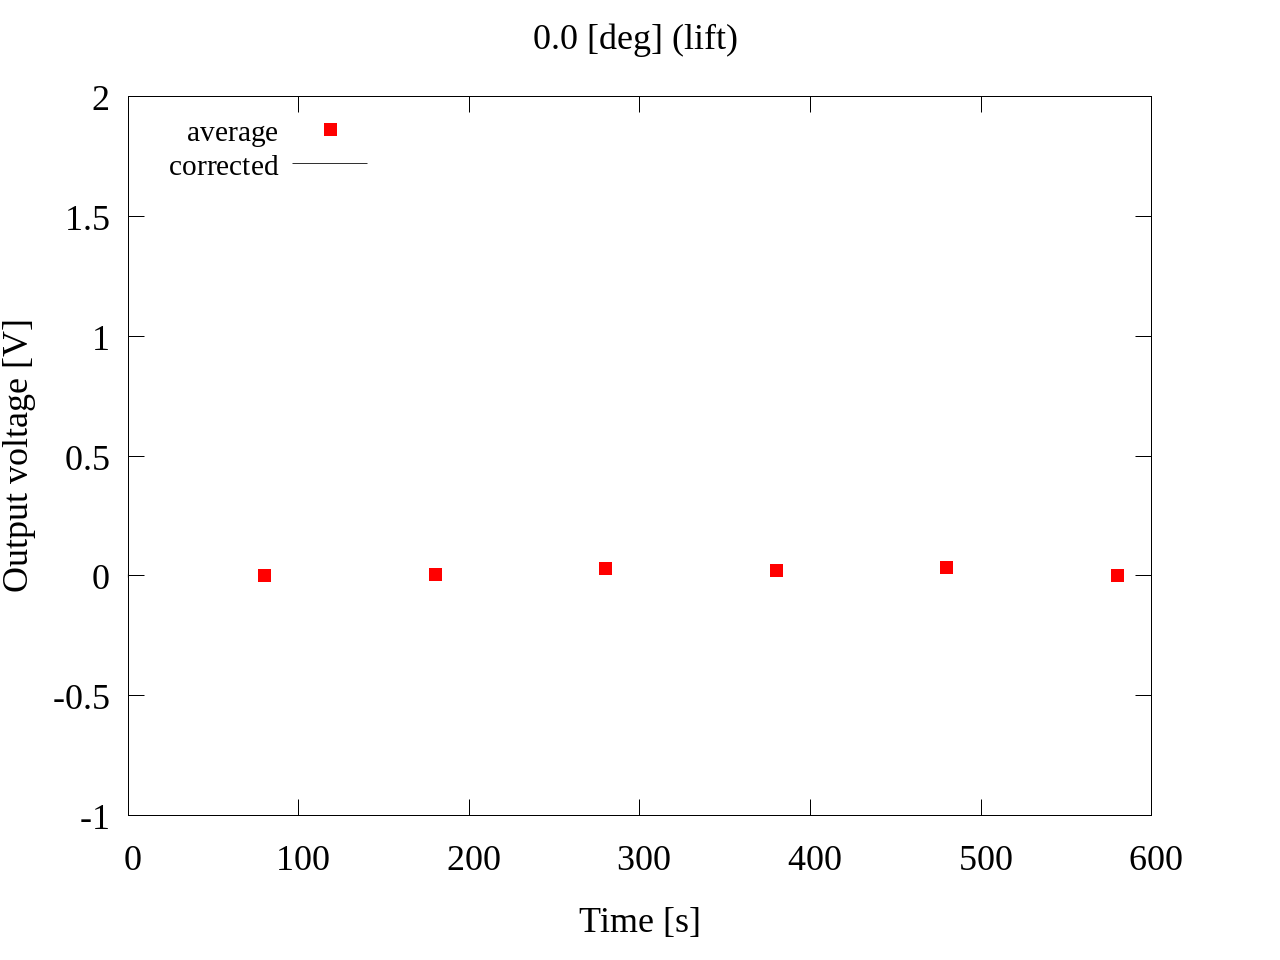
\includegraphics[width=65mm]{../../02_workspace/result/2-1/plot/03-3_lift/03_lift_average_0.png}
		\caption{Drift corrected (lift) : 0 [deg] (1st)}
	\end{minipage}
\end{figure}

\newpage

\subsubsection{出力電圧勾配の算出}

以下のFig.~Fig. に,以上の過程から算出された実験結果の出力電圧勾配を示す.\\
なお,ここでは1回目の実験の算出結果について示している.

\begin{figure}[htbp]
    \begin{minipage}[b]{0.45\linewidth}
      \centering
      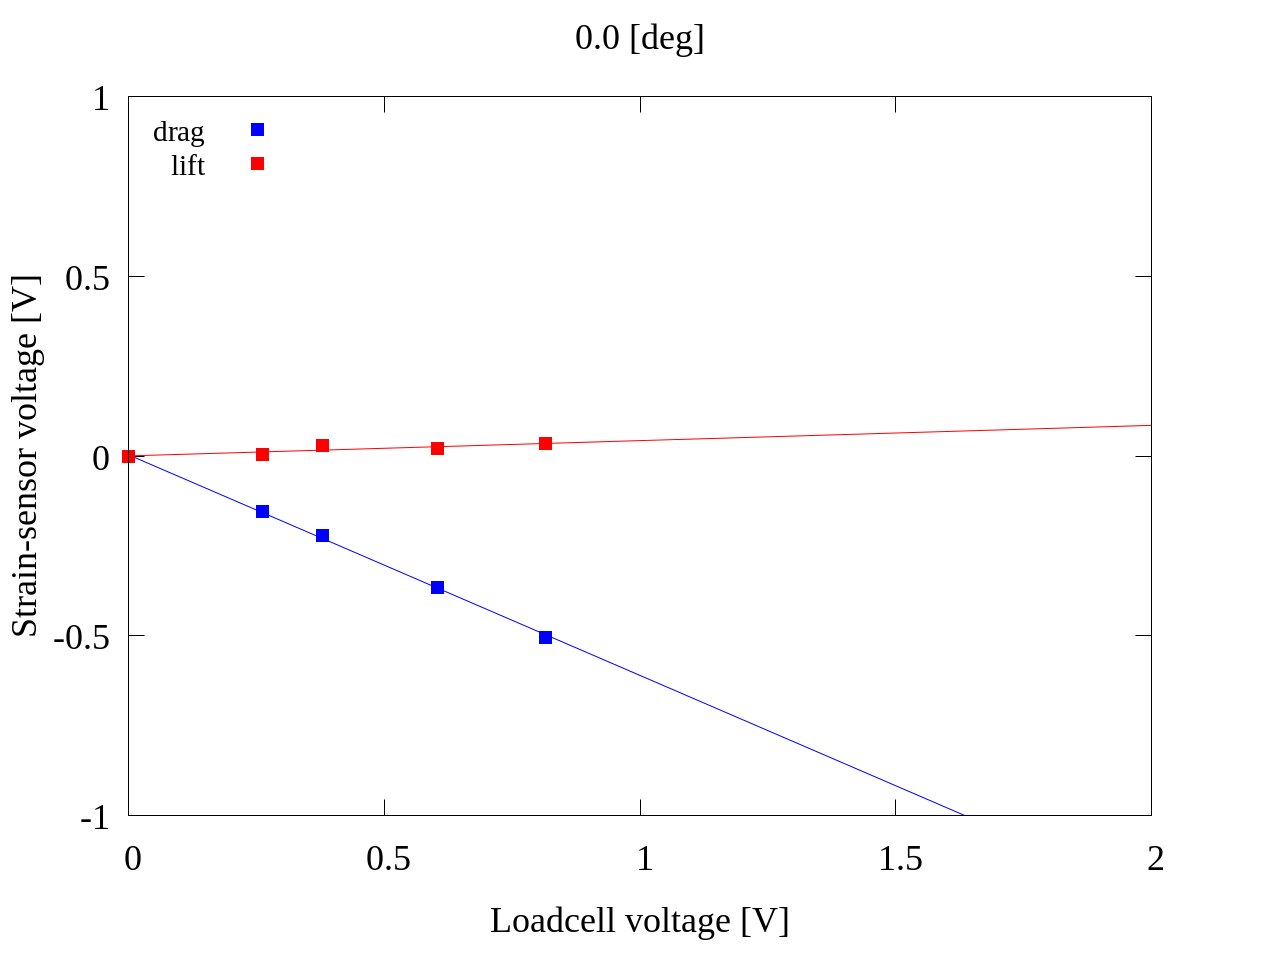
\includegraphics[width=65mm]{../../02_workspace/result/2-1/plot/04/04_linear_0.png}
      \caption{Output voltage : 0 [deg]}
    \end{minipage}
    \begin{minipage}[b]{0.45\linewidth}
      \centering
      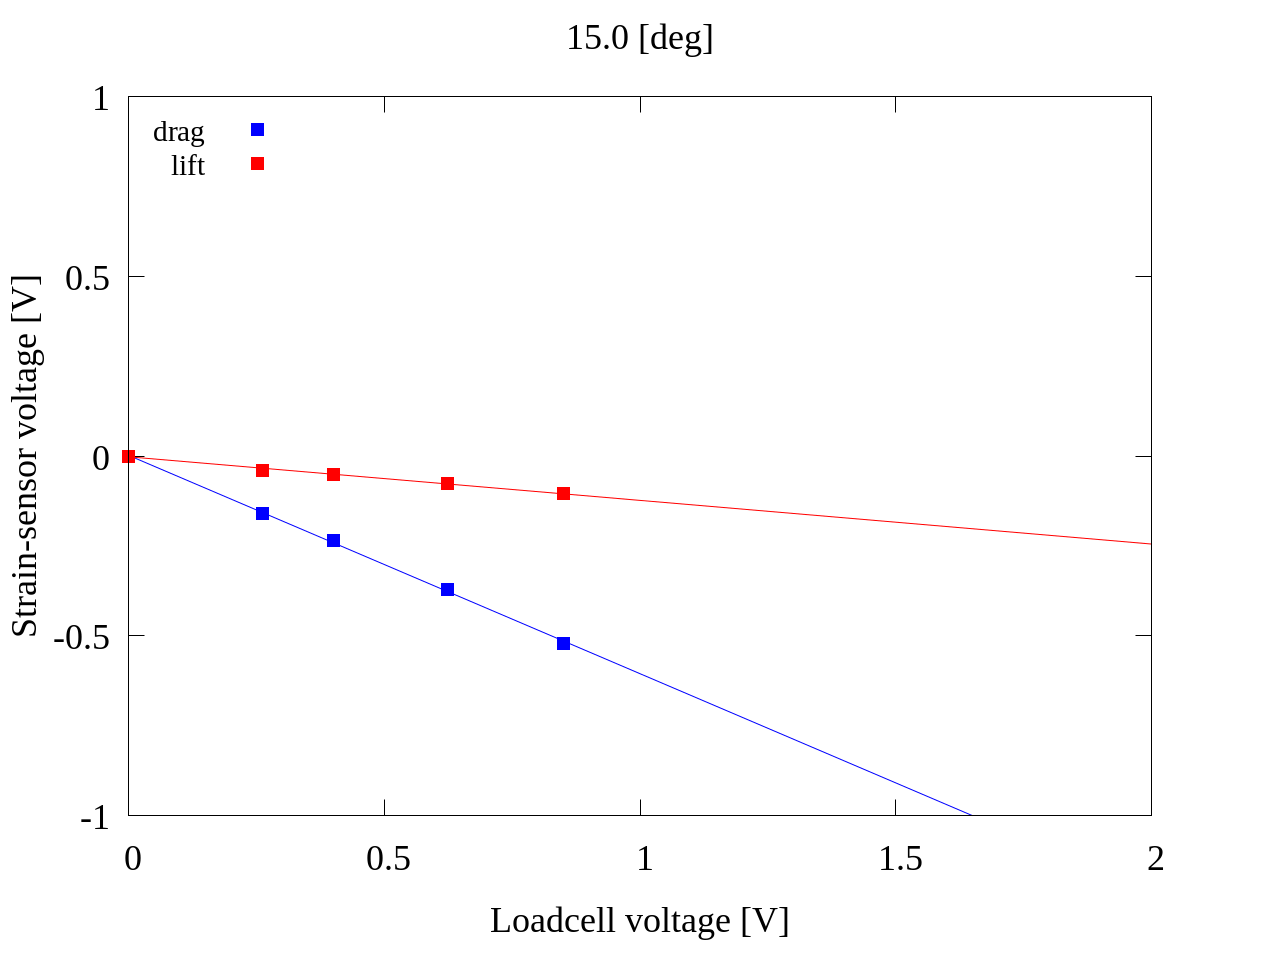
\includegraphics[width=65mm]{../../02_workspace/result/2-1/plot/04/04_linear_150.png}
      \caption{Output voltage : 15 [deg]}
    \end{minipage} \\
    \begin{minipage}[b]{0.45\linewidth}
        \centering
        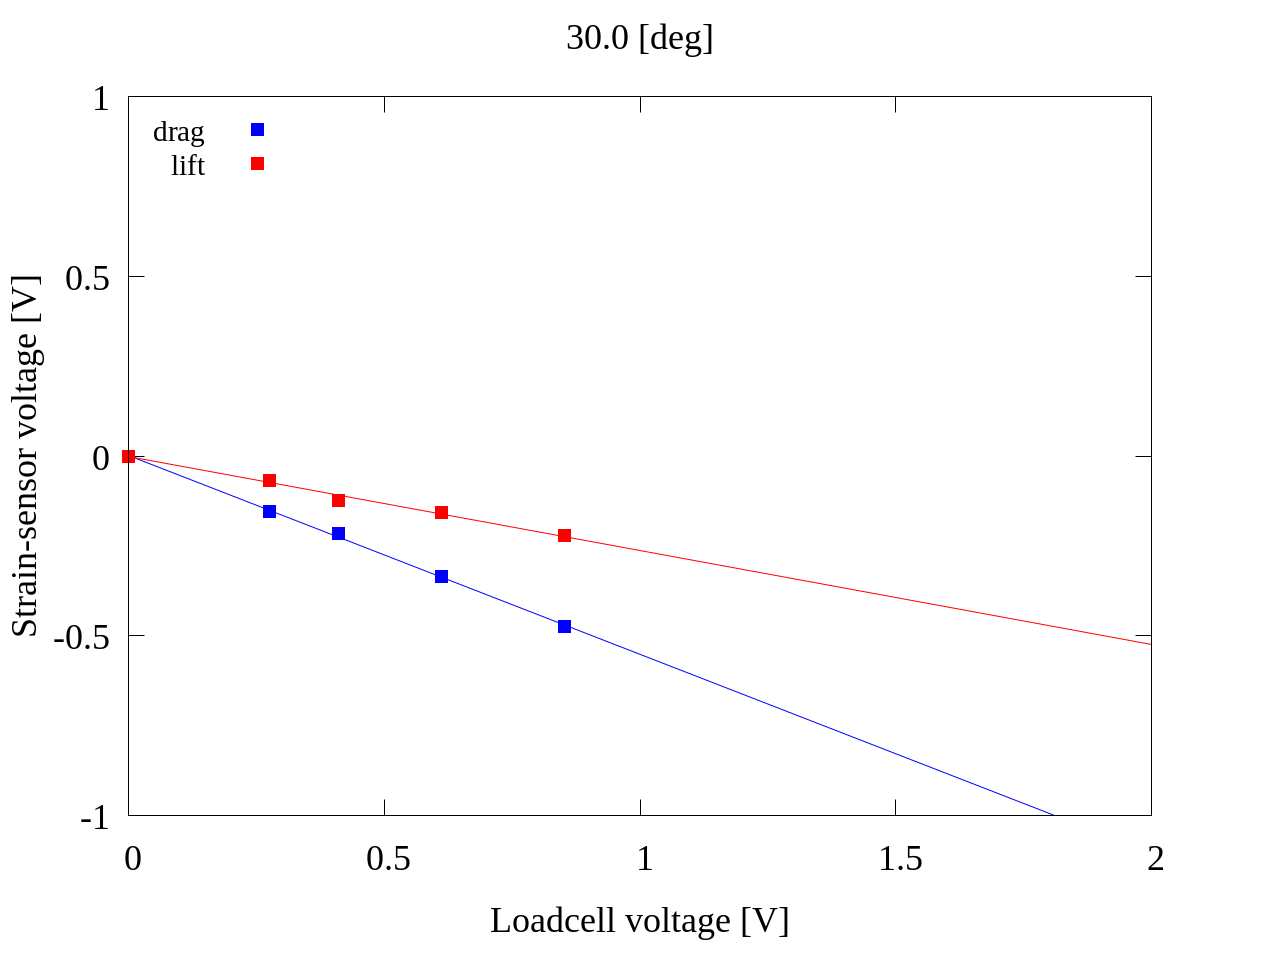
\includegraphics[width=65mm]{../../02_workspace/result/2-1/plot/04/04_linear_300.png}
        \caption{Output voltage : 30 [deg]}
      \end{minipage}
      \begin{minipage}[b]{0.45\linewidth}
        \centering
        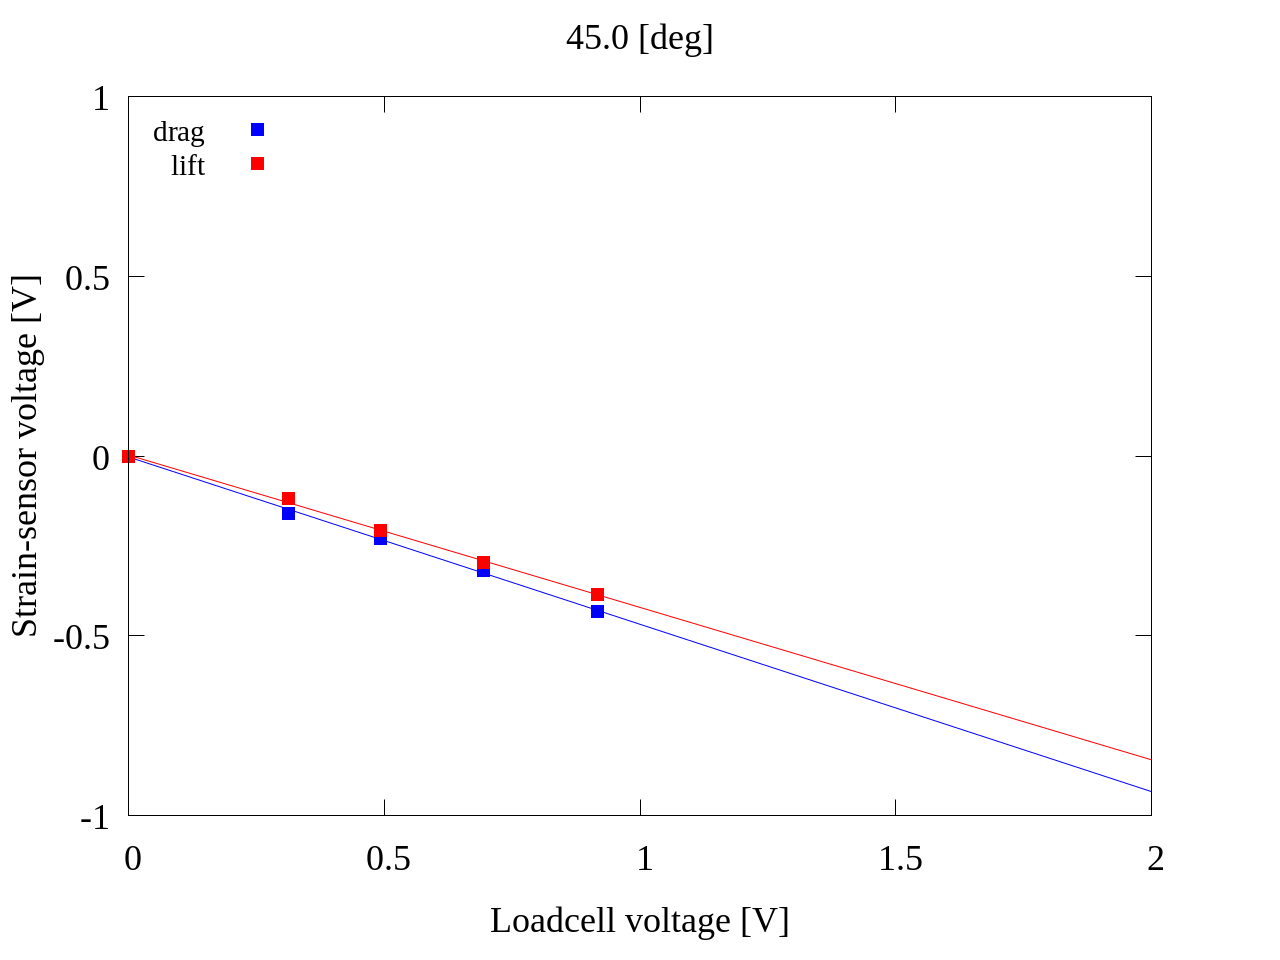
\includegraphics[width=65mm]{../../02_workspace/result/2-1/plot/04/04_linear_450.png}
        \caption{Output voltage : 45 [deg]}
      \end{minipage} \\
      \begin{minipage}[b]{0.45\linewidth}
        \centering
        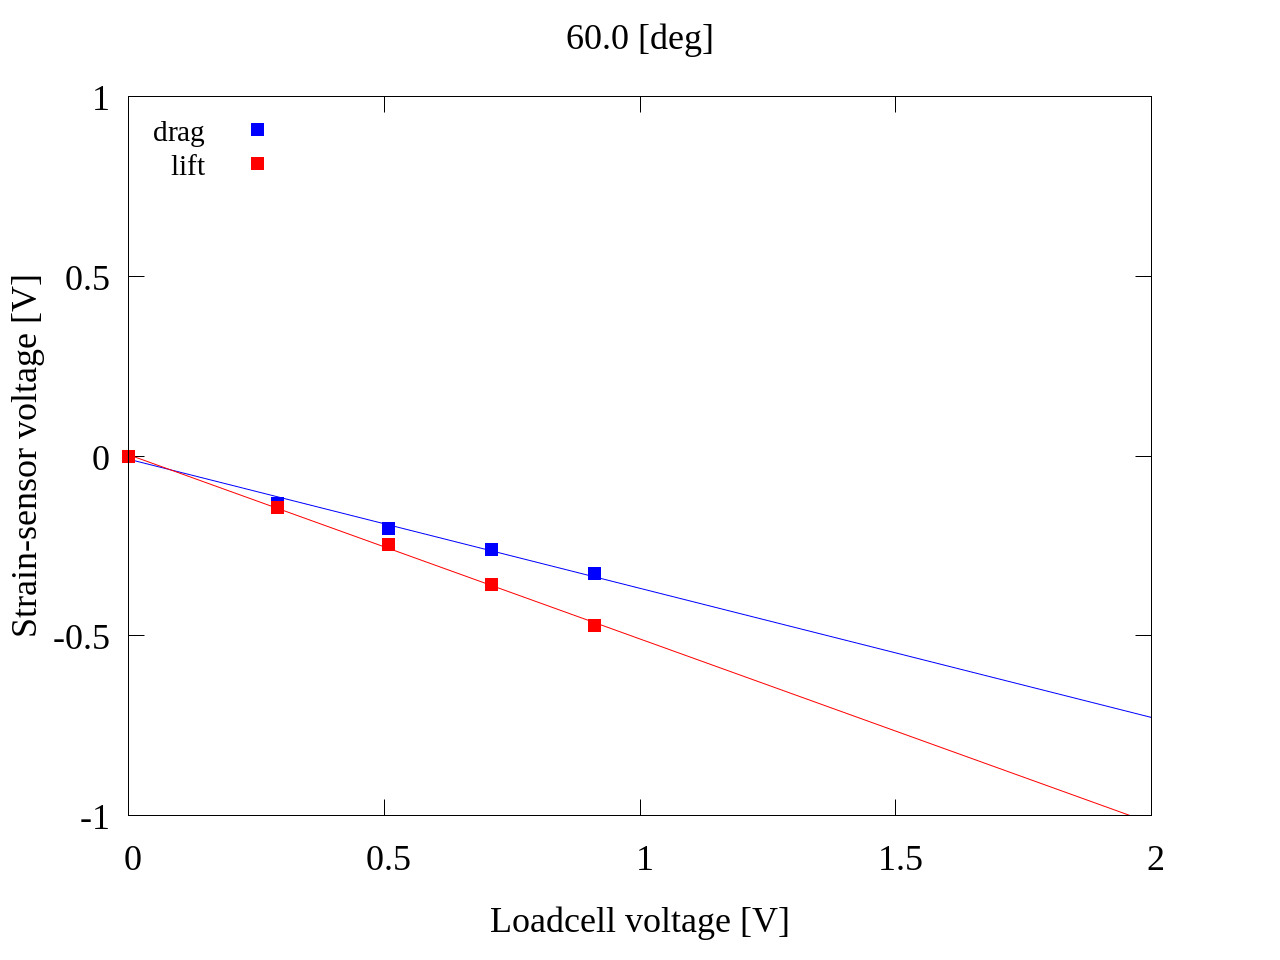
\includegraphics[width=65mm]{../../02_workspace/result/2-1/plot/04/04_linear_600.png}
        \caption{Output voltage : 60 [deg]}
      \end{minipage}
      \begin{minipage}[b]{0.45\linewidth}
        \centering
        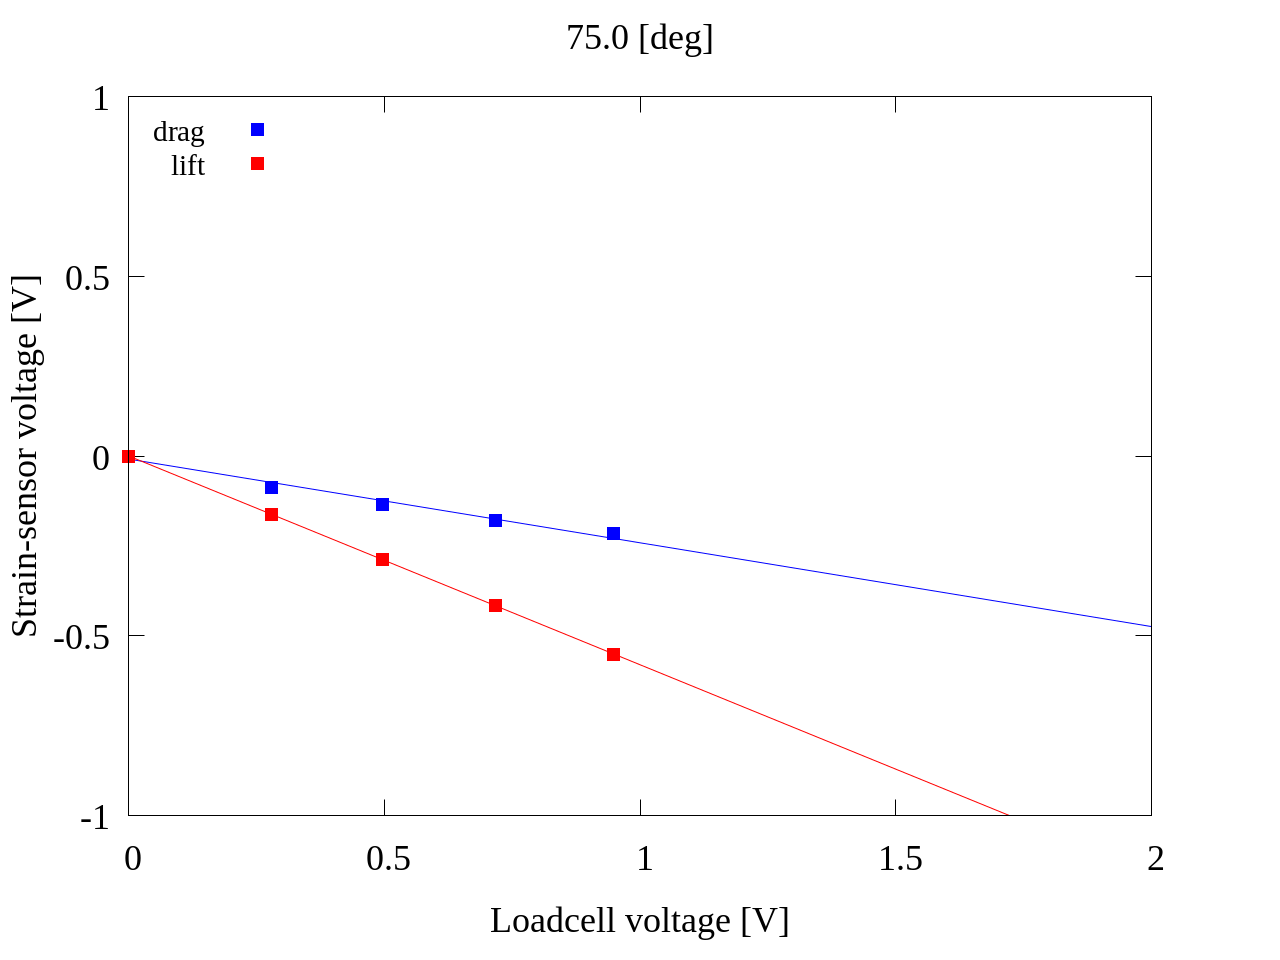
\includegraphics[width=65mm]{../../02_workspace/result/2-1/plot/04/04_linear_750.png}
        \caption{Output voltage : 75 [deg]}
      \end{minipage}
    \end{figure}

    \begin{figure}
      \begin{minipage}[b]{0.45\linewidth}
        \centering
      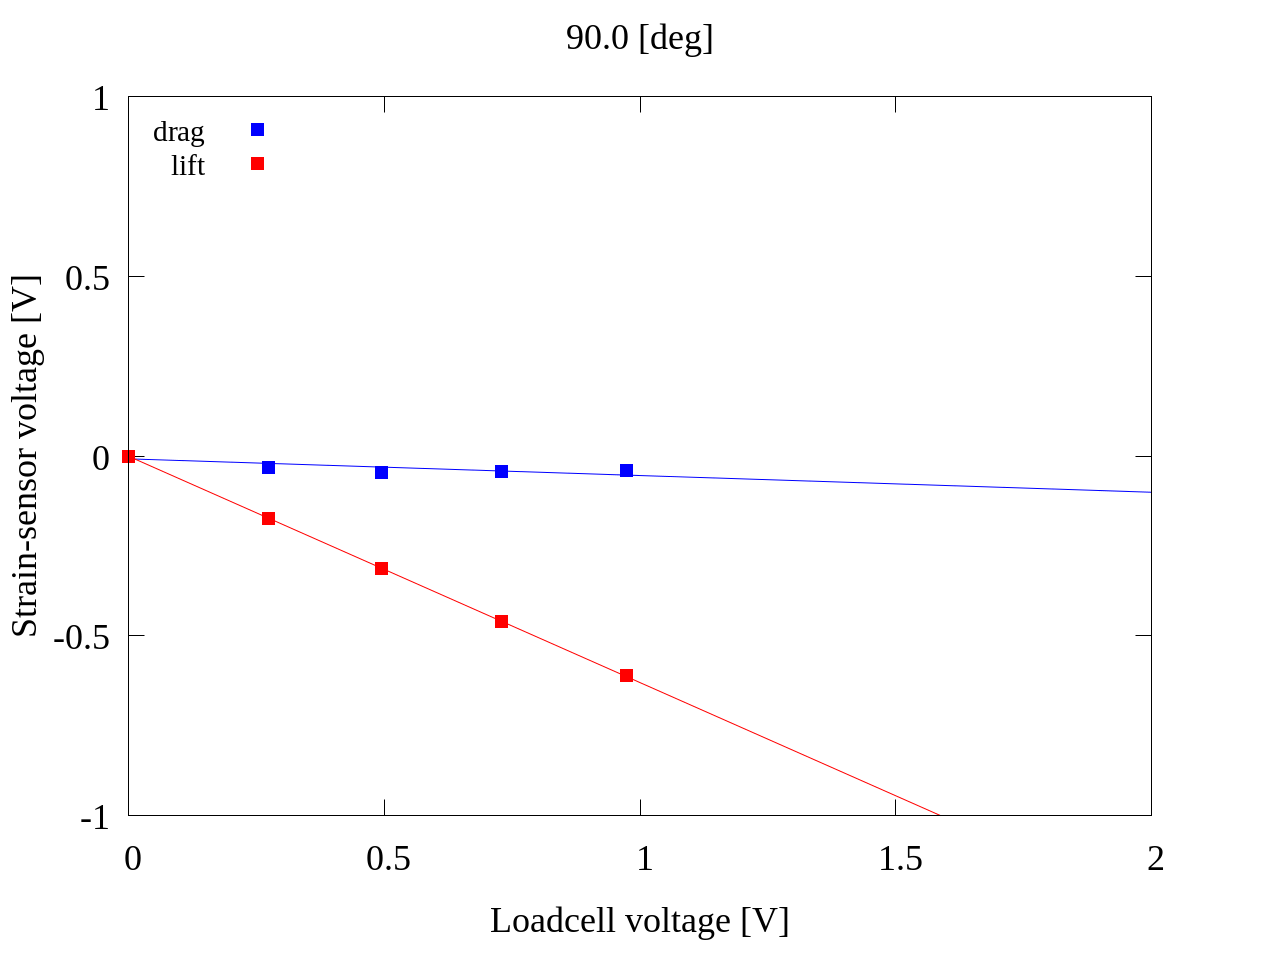
\includegraphics[width=65mm]{../../02_workspace/result/2-1/plot/04/04_linear_900.png}
      \caption{Output voltage : 90 [deg]}
    \end{minipage}
    \begin{minipage}[b]{0.45\linewidth}
        \centering
        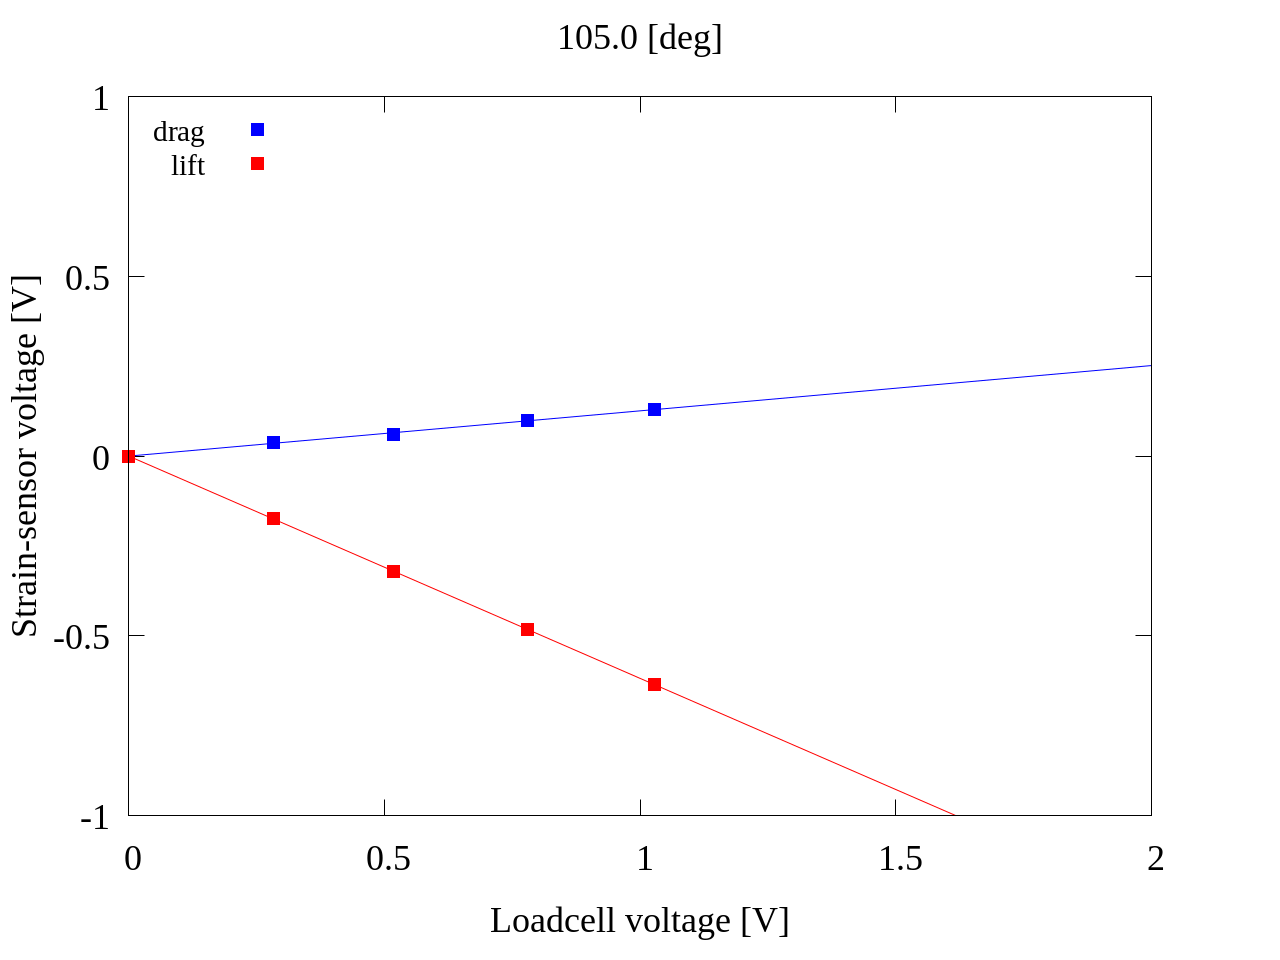
\includegraphics[width=65mm]{../../02_workspace/result/2-1/plot/04/04_linear_1050.png}
        \caption{Output voltage : 105 [deg]}
      \end{minipage}\\
      \begin{minipage}[b]{0.45\linewidth}
        \centering
        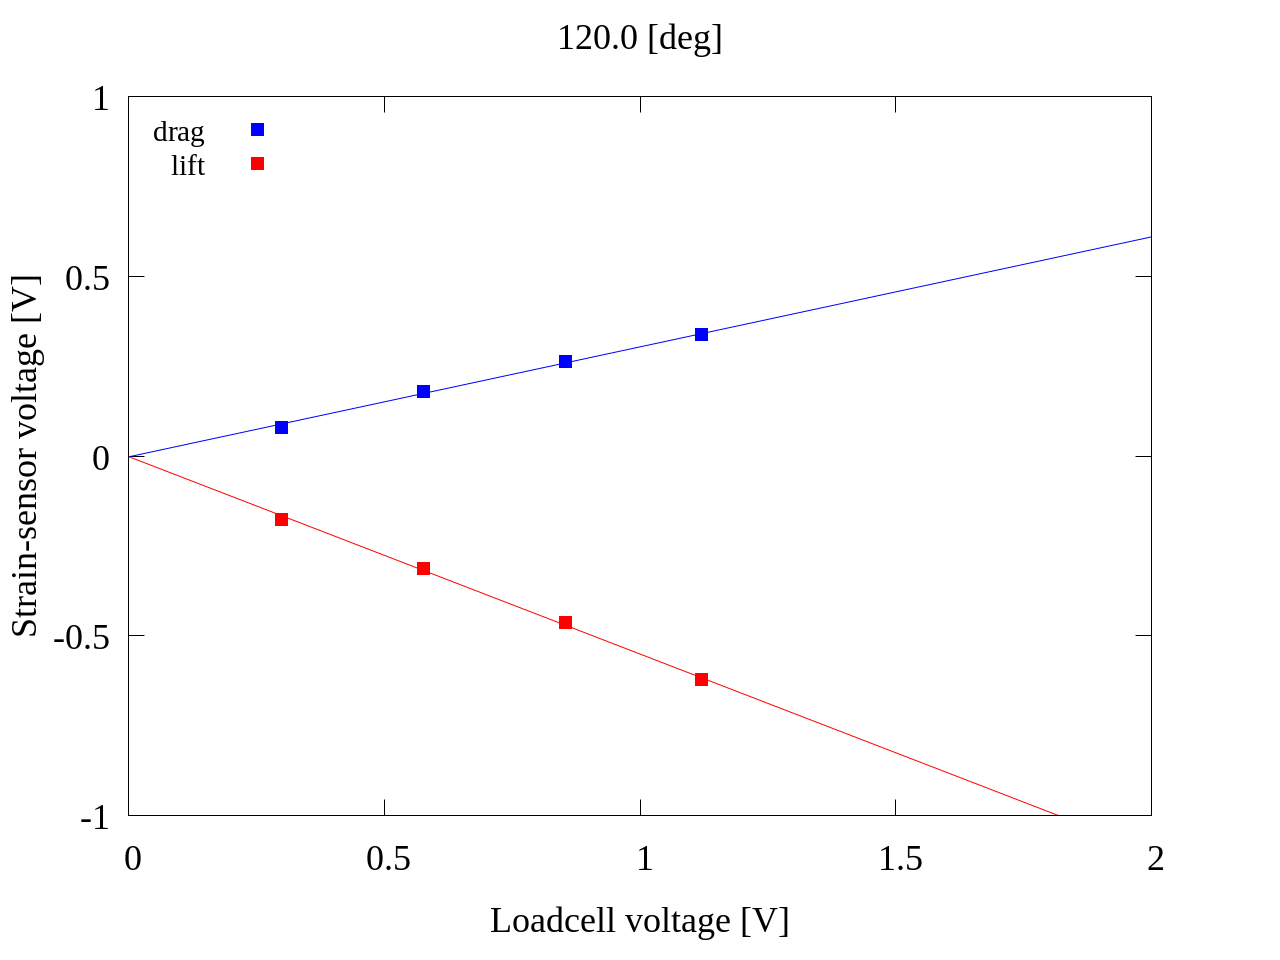
\includegraphics[width=65mm]{../../02_workspace/result/2-1/plot/04/04_linear_1200.png}
        \caption{Output voltage : 120 [deg]}
      \end{minipage}
      \begin{minipage}[b]{0.45\linewidth}
        \centering
        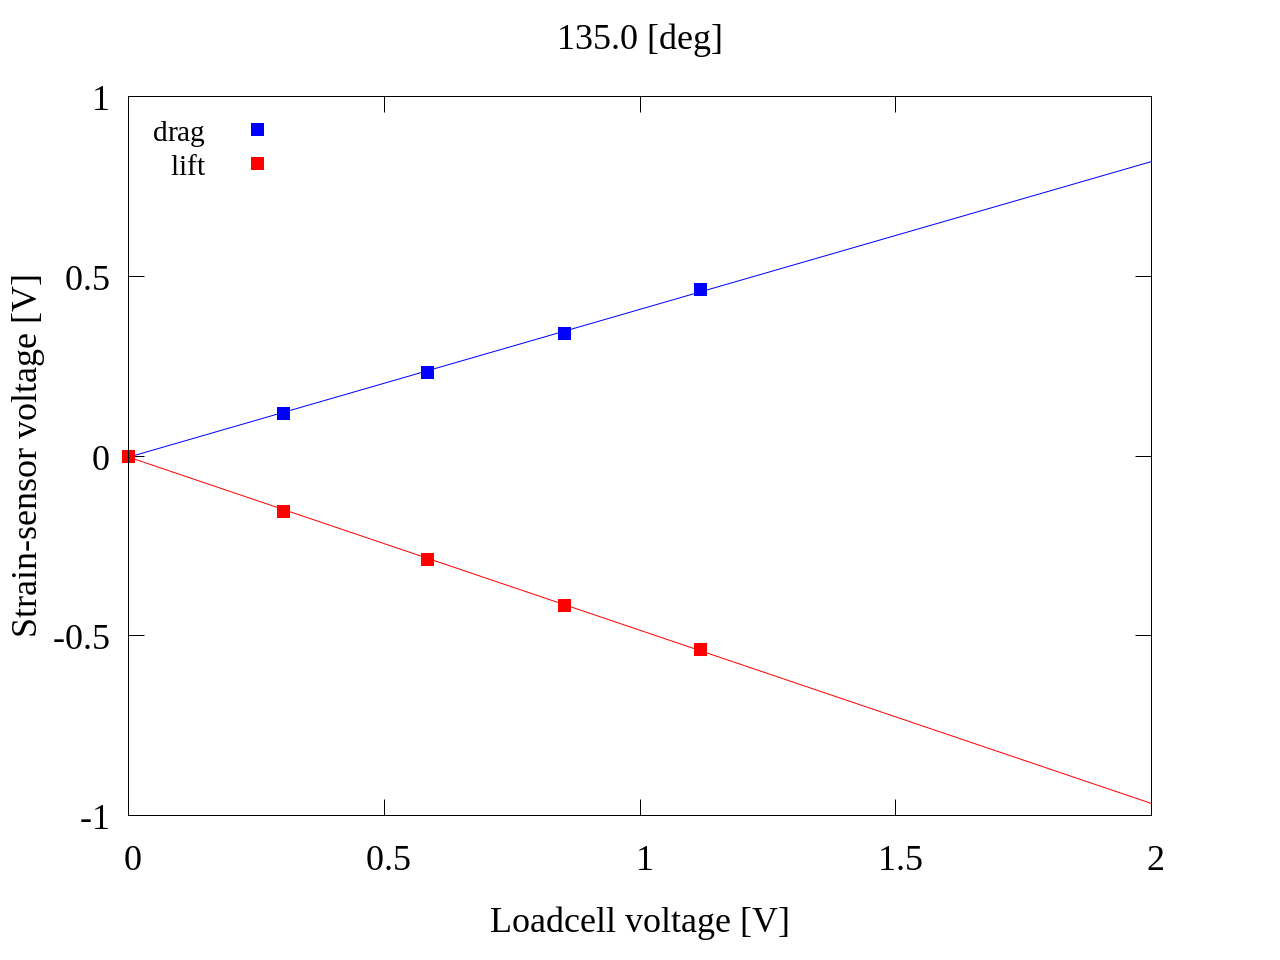
\includegraphics[width=65mm]{../../02_workspace/result/2-1/plot/04/04_linear_1350.png}
        \caption{Output voltage : 135 [deg]}
      \end{minipage}\\
      \begin{minipage}[b]{0.45\linewidth}
        \centering
        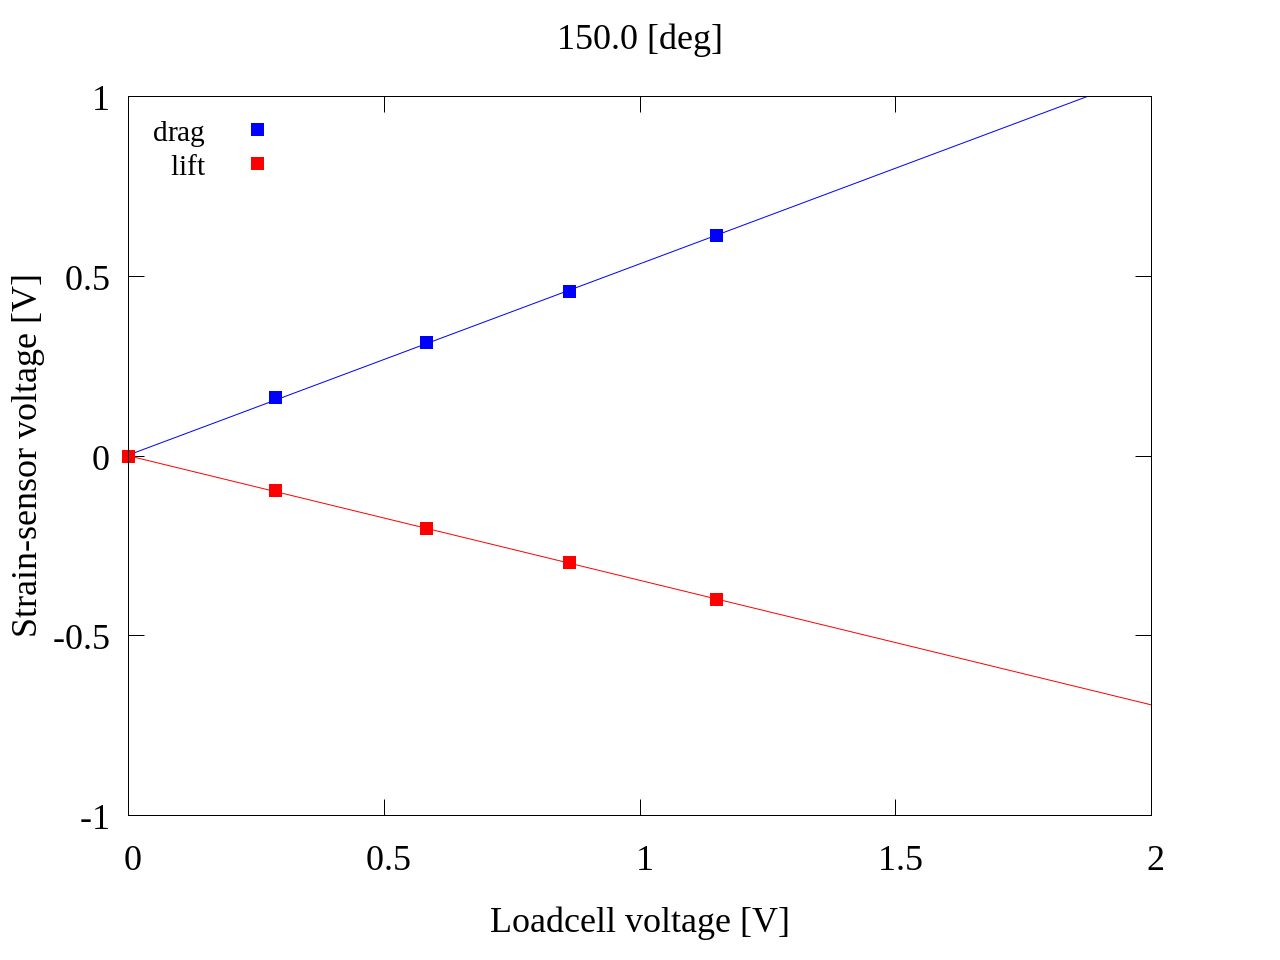
\includegraphics[width=65mm]{../../02_workspace/result/2-1/plot/04/04_linear_1500.png}
        \caption{Output voltage : 150 [deg]}
      \end{minipage} 
      \begin{minipage}[b]{0.45\linewidth}
        \centering
        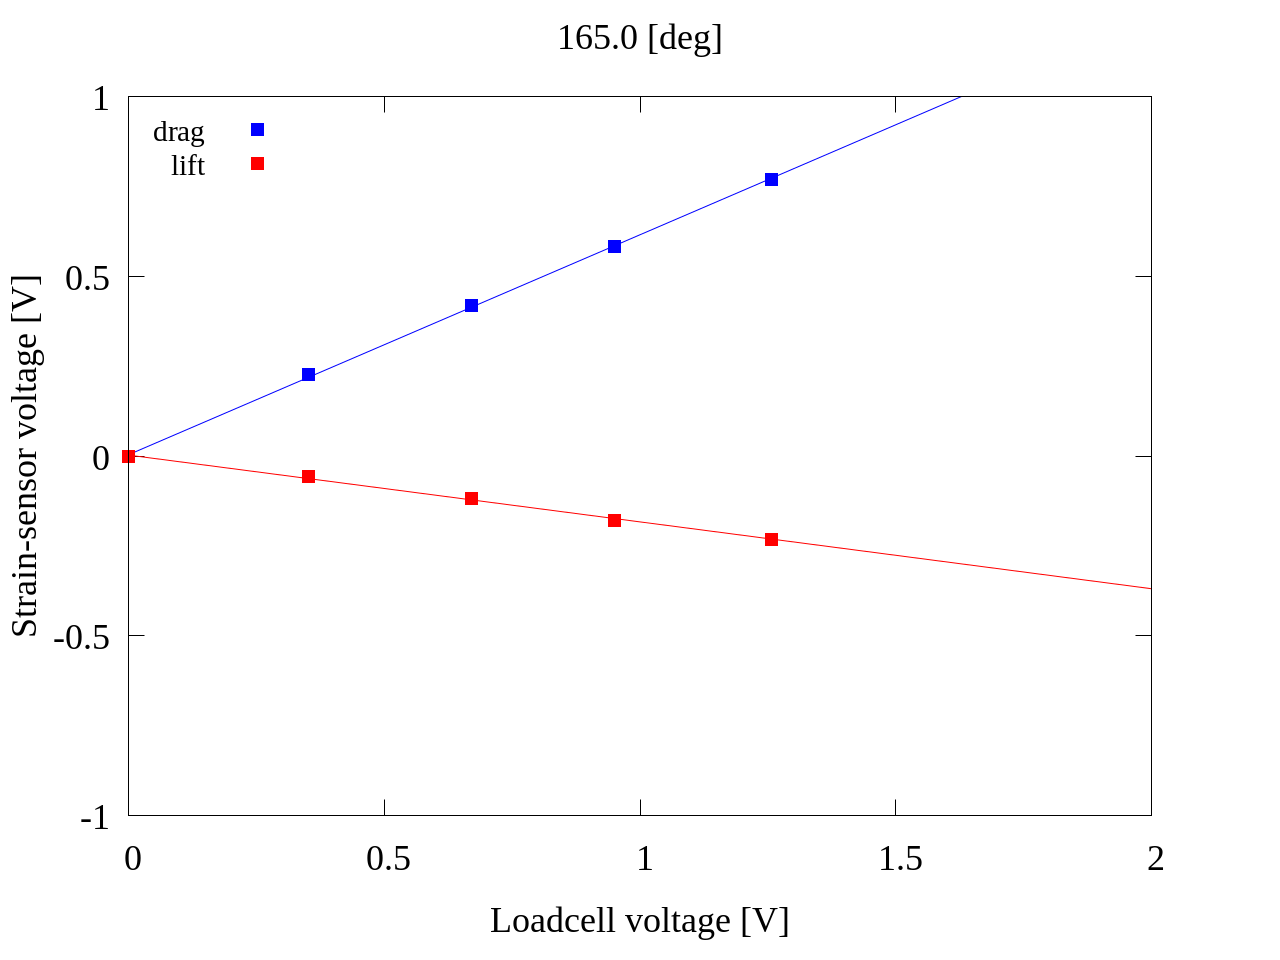
\includegraphics[width=65mm]{../../02_workspace/result/2-1/plot/04/04_linear_1650.png}
        \caption{Output voltage : 165 [deg]}
      \end{minipage}
    \end{figure}

    \begin{figure}
      \begin{minipage}[b]{0.45\linewidth}
        \centering
        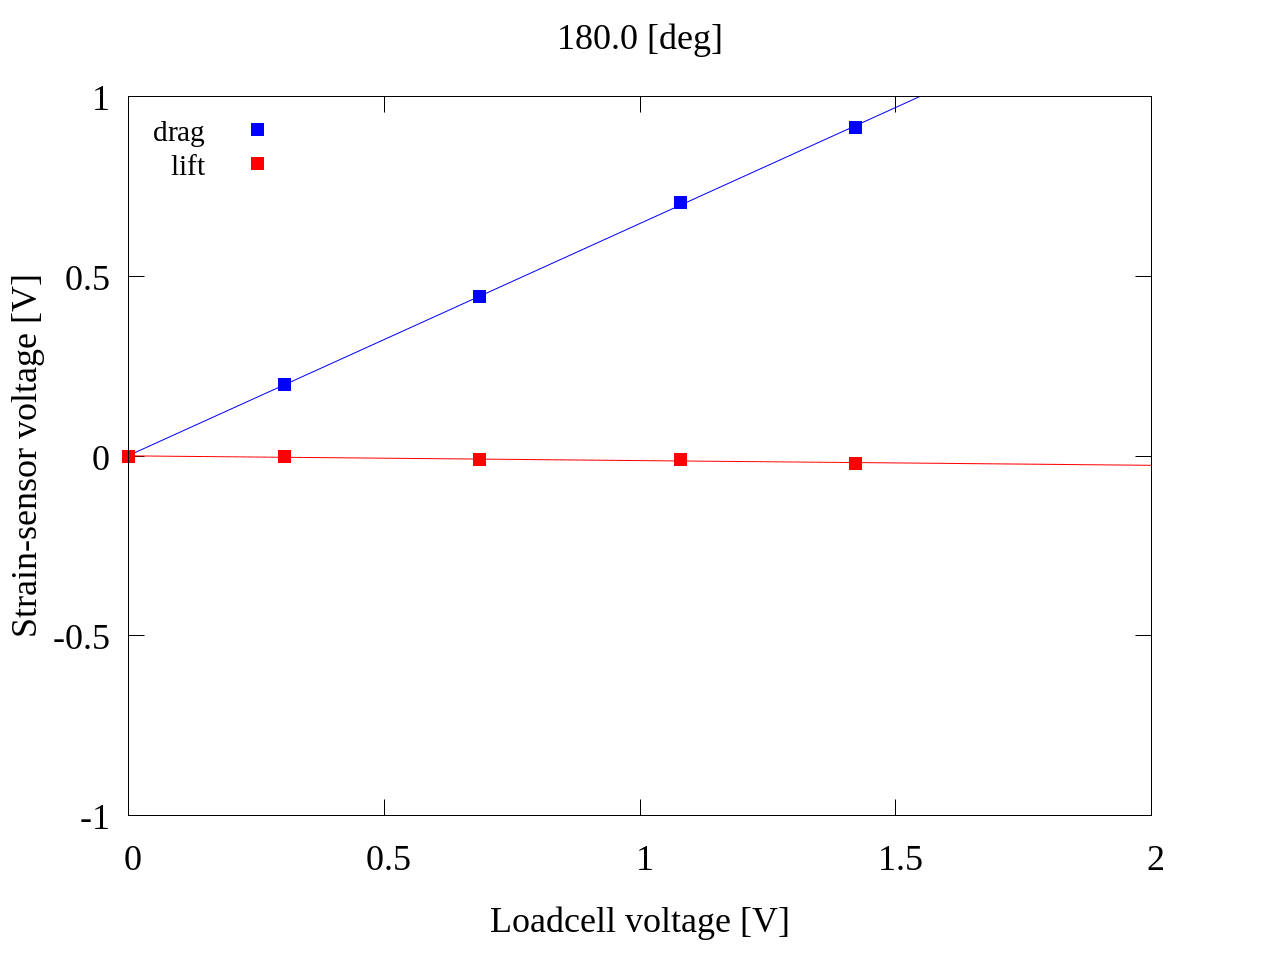
\includegraphics[width=65mm]{../../02_workspace/result/2-1/plot/04/04_linear_1800.png}
        \caption{Output voltage : 180 [deg]}
      \end{minipage}
      \begin{minipage}[b]{0.45\linewidth}
        \centering
        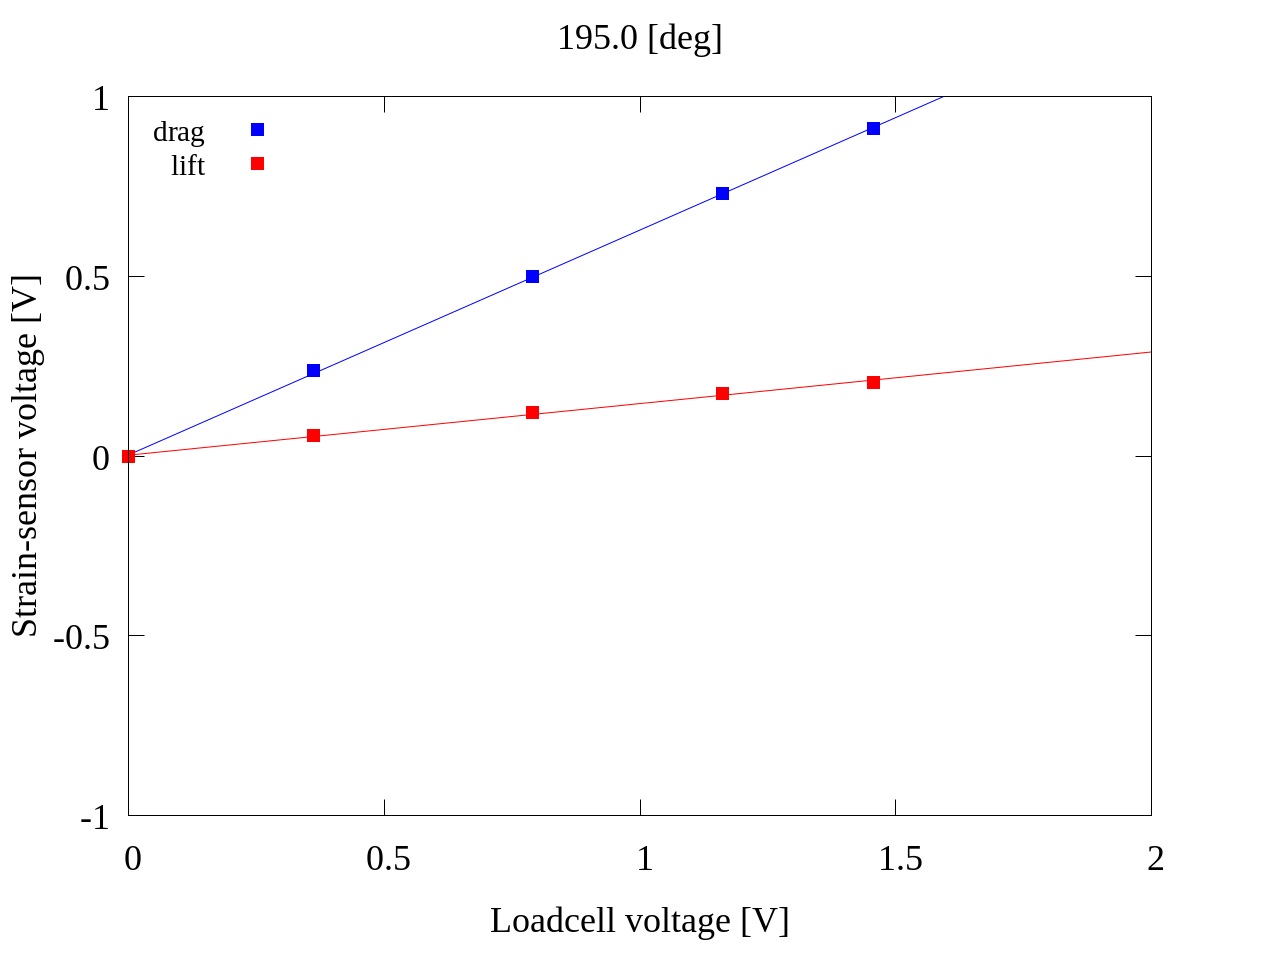
\includegraphics[width=65mm]{../../02_workspace/result/2-1/plot/04/04_linear_1950.png}
        \caption{Output voltage : 195 [deg]}
      \end{minipage}\\
      \begin{minipage}[b]{0.45\linewidth}
        \centering
        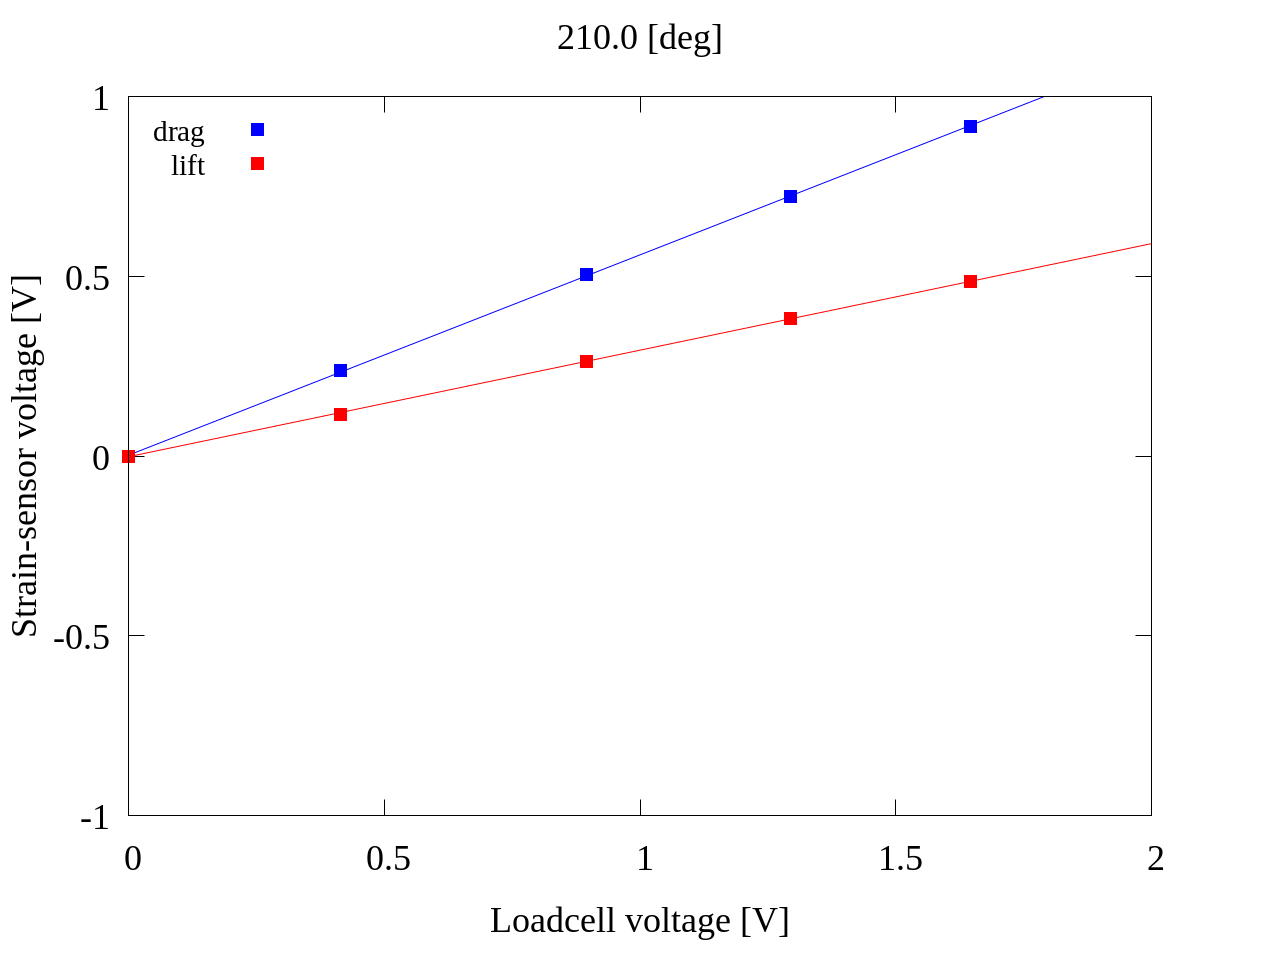
\includegraphics[width=65mm]{../../02_workspace/result/2-1/plot/04/04_linear_2100.png}
        \caption{Output voltage : 210 [deg]}
      \end{minipage}
      \begin{minipage}[b]{0.45\linewidth}
        \centering
        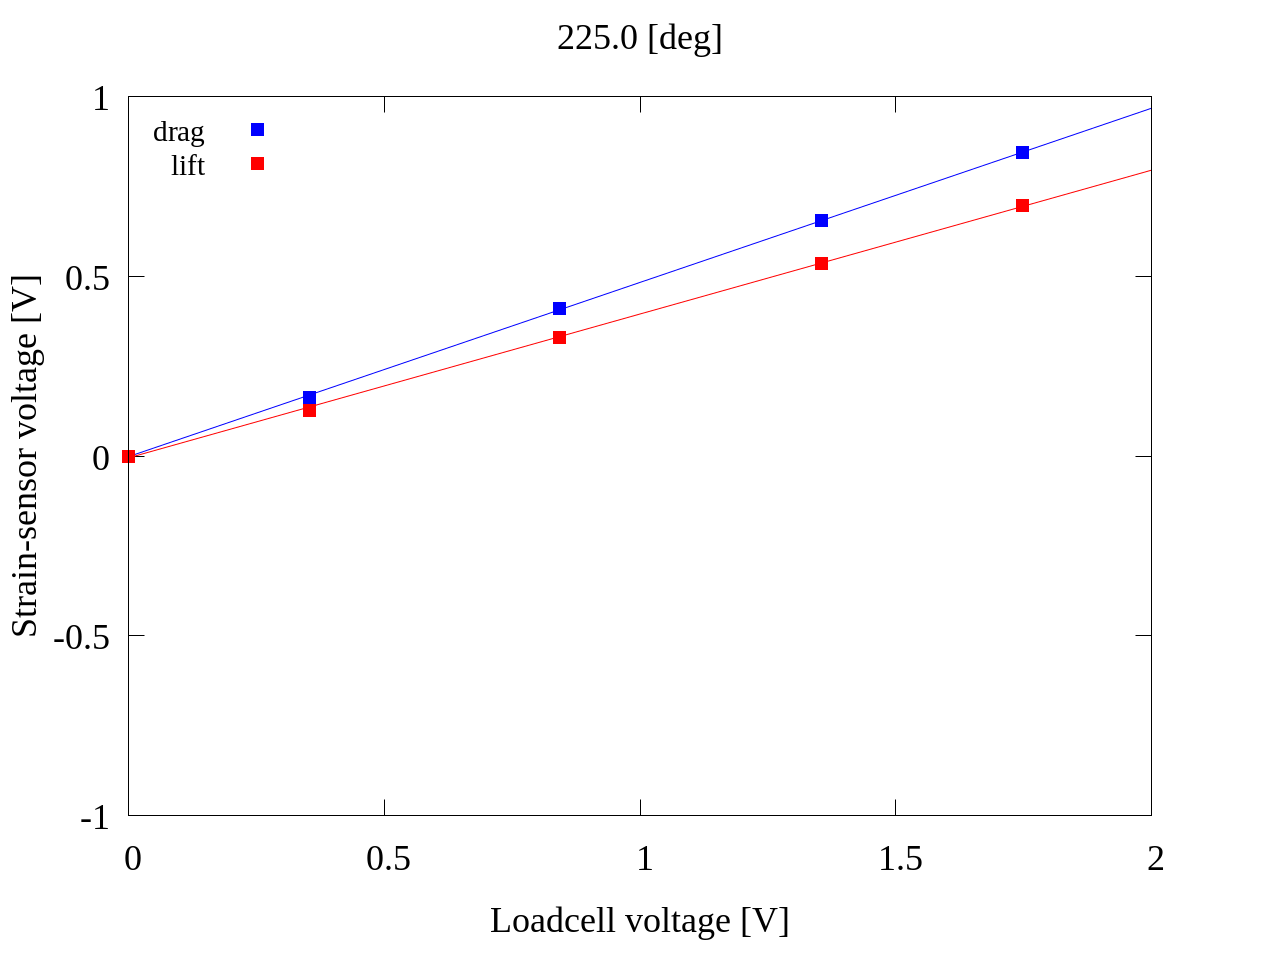
\includegraphics[width=65mm]{../../02_workspace/result/2-1/plot/04/04_linear_2250.png}
        \caption{Output voltage : 225 [deg]}
      \end{minipage}\\
      \begin{minipage}[b]{0.45\linewidth}
        \centering
        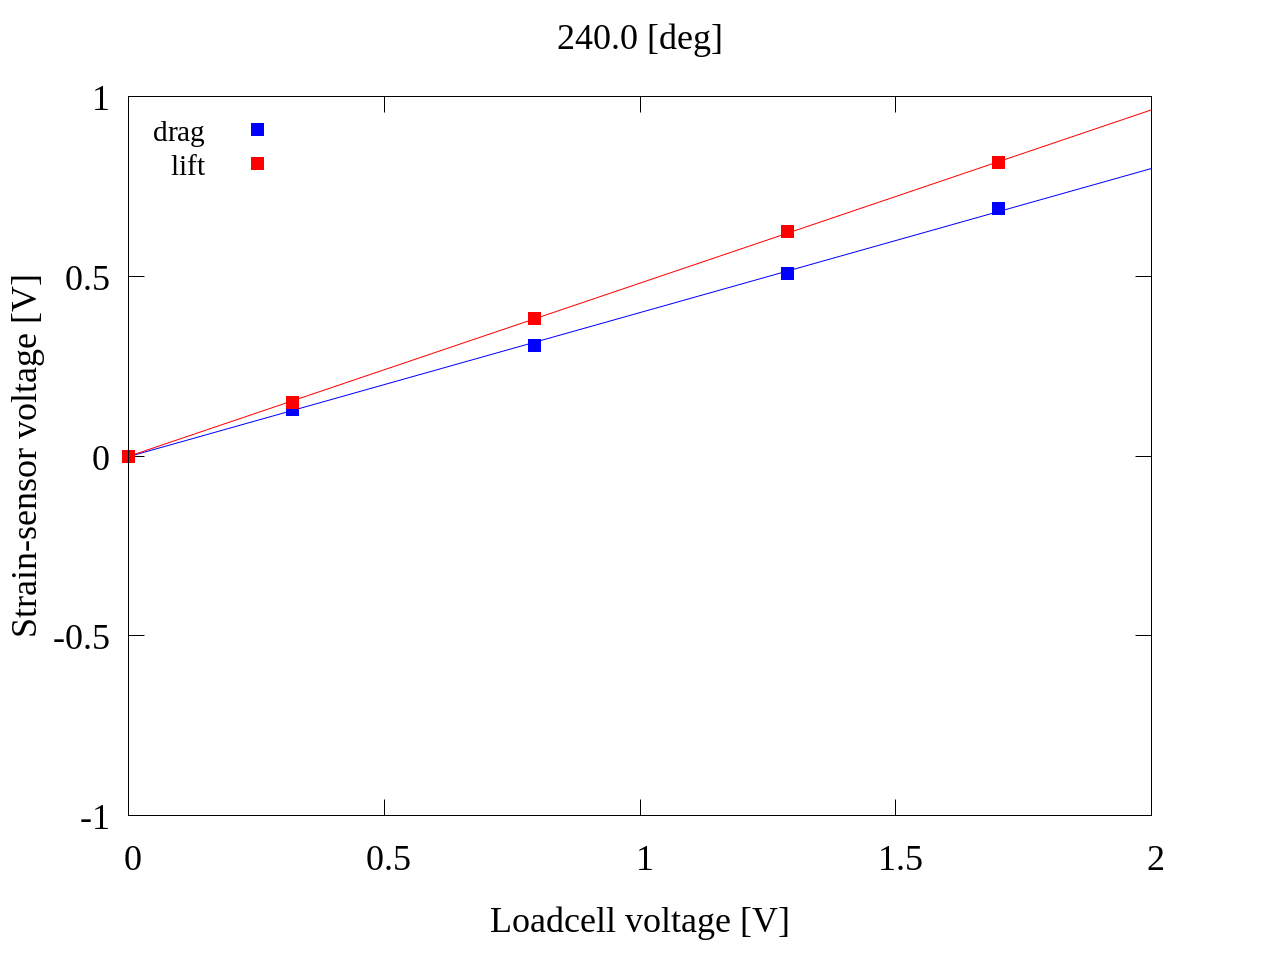
\includegraphics[width=65mm]{../../02_workspace/result/2-1/plot/04/04_linear_2400.png}
        \caption{Output voltage : 240 [deg]}
      \end{minipage}
      \begin{minipage}[b]{0.45\linewidth}
        \centering
        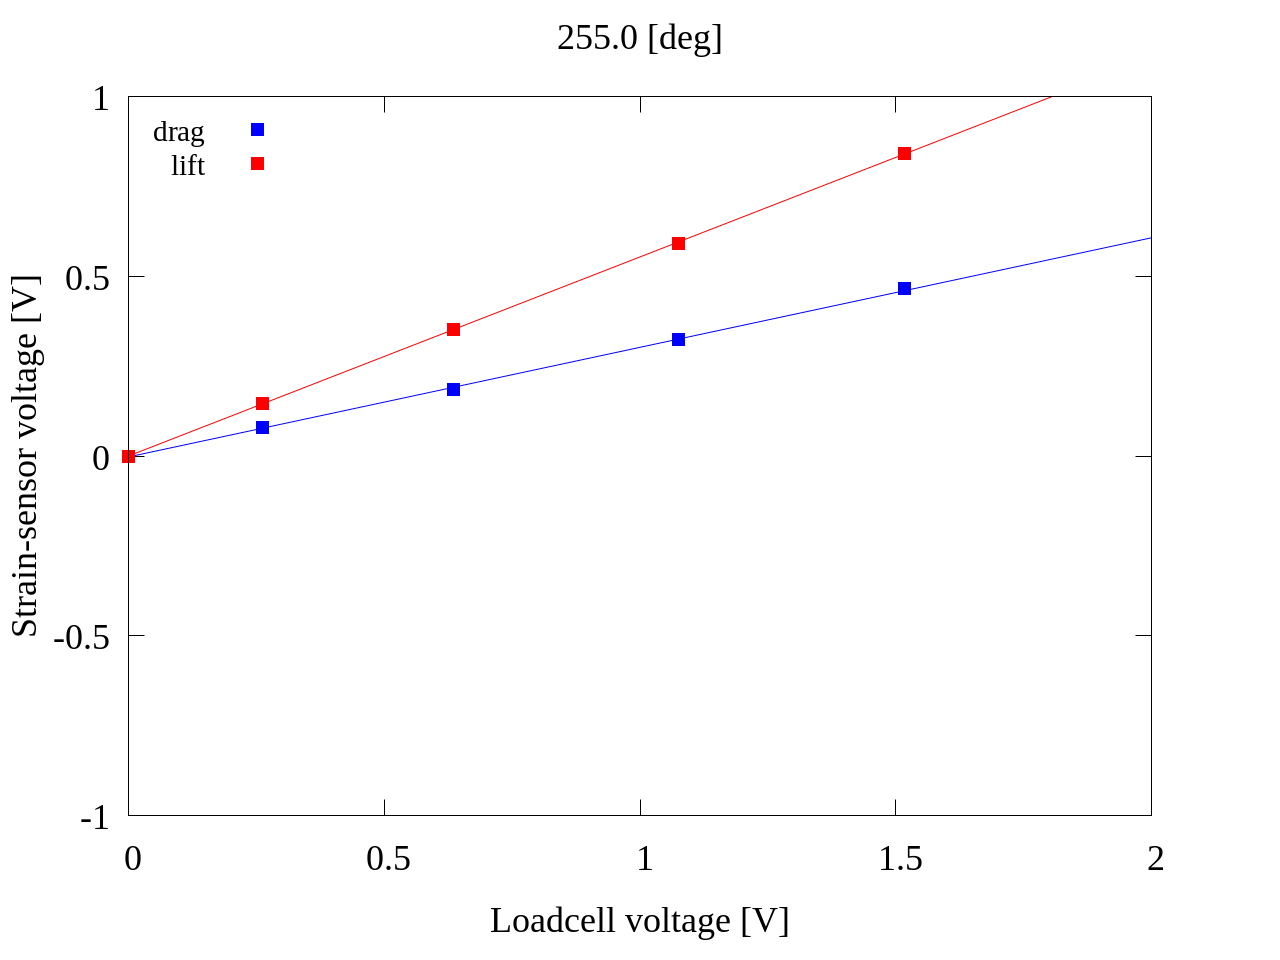
\includegraphics[width=65mm]{../../02_workspace/result/2-1/plot/04/04_linear_2550.png}
        \caption{Output voltage : 255 [deg]}
      \end{minipage}
    \end{figure}

    \begin{figure}
      \begin{minipage}[b]{0.45\linewidth}
        \centering
        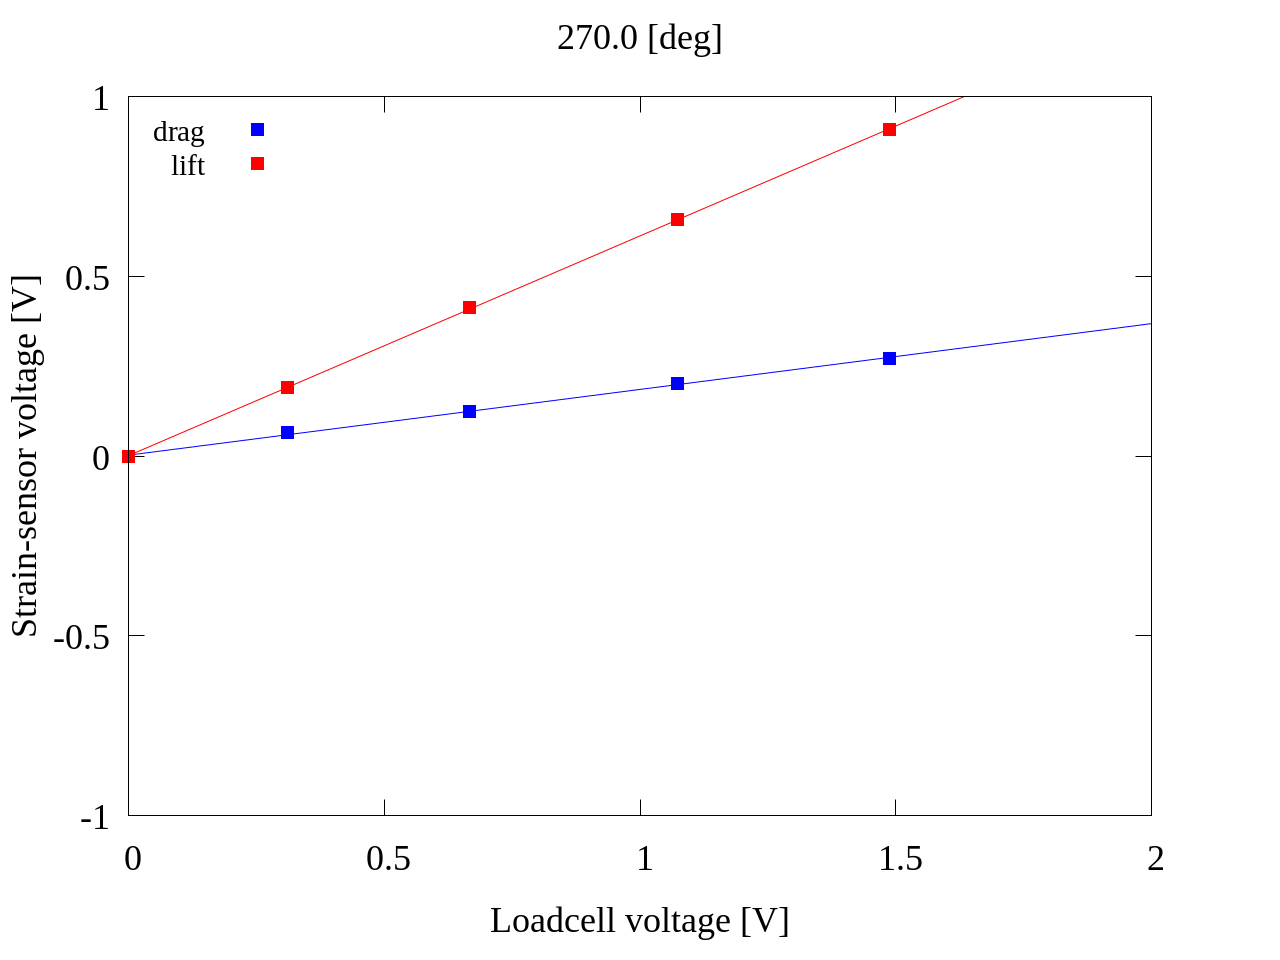
\includegraphics[width=65mm]{../../02_workspace/result/2-1/plot/04/04_linear_2700.png}
        \caption{Output voltage : 270 [deg]}
      \end{minipage}
      \begin{minipage}[b]{0.45\linewidth}
        \centering
        \includegraphics[width=65mm]{../../02_workspace/result/2-1/plot/04/04_linear_2850.png}
        \caption{Output voltage : 285 [deg]}
      \end{minipage}\\
      \begin{minipage}[b]{0.45\linewidth}
        \centering
        \includegraphics[width=65mm]{../../02_workspace/result/2-1/plot/04/04_linear_3000.png}
        \caption{Output voltage : 300 [deg]}
      \end{minipage}
      \begin{minipage}[b]{0.45\linewidth}
        \centering
        \includegraphics[width=65mm]{../../02_workspace/result/2-1/plot/04/04_linear_3150.png}
        \caption{Output voltage : 315 [deg]}
      \end{minipage}\\
      \begin{minipage}[b]{0.45\linewidth}
        \centering
        \includegraphics[width=65mm]{../../02_workspace/result/2-1/plot/04/04_linear_3300.png}
        \caption{Output voltage : 330 [deg]}
      \end{minipage}
      \begin{minipage}[b]{0.45\linewidth}
        \centering
        \includegraphics[width=65mm]{../../02_workspace/result/2-1/plot/04/04_linear_3450.png}
        \caption{Output voltage : 345 [deg]}
      \end{minipage}
\end{figure}

\newpage

また,出力電圧勾配について各角度における算出値をプロットしたものを以下のFig.,Fig.に示す.
なお,ここで示す出力電圧勾配の値は5回実施した実験結果の平均値である.

\begin{figure}[htbp]
		\centering
		\includegraphics[width=95mm]{../../02_workspace/result/2-ex/plot/21/21-1_summary_drag.png}
		\caption{Gradient of voltage : drag (Average)}
		\includegraphics[width=95mm]{../../02_workspace/result/2-ex/plot/21/21-1_summary_lift.png}
		\caption{Gradient of voltage : lift (Average)}
\end{figure}

\newpage

\subsection{校正理論の適用とその結果}
Fig.について作成した補正理論を適用し,
水槽座標系における出力電圧勾配への変換を行う.

\subsubsection{座標系のオフセットにおける補正理論の適用}
Fig.,Fig.について,座標系のオフセットにおける補正理論である
式()の適用後の出力電圧勾配$v_{x'1}$,$v_{y'1}$を以下のFig.,Fig.に示す.
なお,補正の際に用いたオフセット距離$\Delta x$,$\Delta y$は
実験の際に測定した以下のTable の数値を用いて行った.

\begin{table}[htbp]
  \begin{center}
      \caption{Offset velue}
      \begin{tabular}{|p{30mm}|p{20mm}|p{20mm}|}
          \hline
          \multicolumn{1}{|c|}{$\Delta x$ [mm]} & \multicolumn{1}{|c|}{$\Delta y$ [mm]} \\ \hline
          \multicolumn{1}{|c|}{0.09}           & \multicolumn{1}{|c|}{0.06}           \\ \hline
      \end{tabular}
  \end{center}
\end{table}

\begin{figure}[htbp]
		\centering
		\includegraphics[width=95mm]{../../02_workspace/result/2-ex/plot/21/21-2_corrected_offset_drag.png}
		\caption{Offset corrected : drag (Average)}
		\includegraphics[width=95mm]{../../02_workspace/result/2-ex/plot/21/21-2_corrected_offset_lift.png}
		\caption{Offset corrected : lift (Average)}
\end{figure}

\newpage

\subsubsection{ラグランジュ補間公式の適用}
Fig.,Fig.について,式()のラグランジュ補間公式によって
二次補間の適用後の出力電圧勾配$v_{x'2}$,$v_{y'2}$を以下のFig.,Fig.に示す.

\begin{figure}[htbp]
		\centering
		\includegraphics[width=95mm]{../../02_workspace/result/2-ex/plot/21/21-3_interpolated_drag.png}
		\caption{Interpolated : drag (Average)}
		\includegraphics[width=95mm]{../../02_workspace/result/2-ex/plot/21/21-3_interpolated_lift.png}
		\caption{Interpolated : lift (Average)}
\end{figure}

\newpage

Fig.,Fig.について

\subsubsection{座標系の回転における補正理論の適用}
はじめに,水槽座標系からの回転角$\theta_x$,$\theta_y$を推定するため,
Fig.,Fig.の結果に離散フーリエ変換を適用し,波数1の成分から$\theta_x$,$\theta_y$を算出する.
ここで,Fig.,Fig.について,離散フーリ変換を適用した結果を以下のFig.,Fig.に示す.

\begin{figure}
        \begin{minipage}[b]{0.45\linewidth}
        \centering
        \includegraphics[width=65mm]{../../02_workspace/result/2-ex/plot/07/07-3_dft-drag.png}
        \caption{DFT spectrum (drag) (average)}
      \end{minipage}
      \begin{minipage}[b]{0.45\linewidth}
        \centering
        \includegraphics[width=65mm]{../../02_workspace/result/2-ex/plot/07/07-4_dft-lift.png}
        \caption{DFT spectrum (lift) (average)}
      \end{minipage}
\end{figure}

Fig.,Fig.をみると,どちらもピークは波数1のときにあり,
波の特徴を正しく捉えられていることがわかる.
また,このとき算出された波数1の値について,以下のTable に示す.

\begin{table}[htbp]
  \begin{center}
      \caption{DFT result value : wave 1}
      \begin{tabular}{|p{30mm}|p{20mm}|p{20mm}|}
          \hline
          \multicolumn{1}{|c|}{}     & \multicolumn{1}{|c|}{Re}    & \multicolumn{1}{|c|}{Im}   \\ \hline
          \multicolumn{1}{|c|}{Drag} & \multicolumn{1}{|c|}{-7.503} & \multicolumn{1}{|c|}{1.022}  \\ \hline
          \multicolumn{1}{|c|}{Lift} & \multicolumn{1}{|c|}{0.664}  & \multicolumn{1}{|c|}{7.559} \\ \hline
      \end{tabular}
  \end{center}
\end{table}

ここで,式(),式()を用いてそれぞれの回転角$\theta_x$,$\theta_y$を算出する.
余弦波からの位相角をそれぞれ$\phi_x$,$\phi_y$とすると,以下のように算出される.
\begin{align}
	\phi_x &= \arctan \left(\frac{1.022}{-7.503}\right) \cdot \frac{180}{\pi} = \\
	\phi_y &= \arctan \left(\frac{0.664}{7.559}\right) \cdot \frac{180}{\pi} = 
\end{align}

したがって,回転角$\theta_x$,$\theta_y$は,以下のように表される.
\begin{align}
	\theta_x &= 180 - \phi_x = 7.757 \; [\mathrm{deg}]\\
	\theta_y &= 90 - \phi_y = 5.019 \; [\mathrm{deg}]
\end{align}

また,その算出結果を以下のTable に示す.

\begin{table}[htbp]
  \begin{center}
      \caption{Specified rotation angle}
      \begin{tabular}{|p{30mm}|p{20mm}|p{20mm}|}
          \hline
          \multicolumn{1}{|c|}{$\theta_x$ [deg]} & \multicolumn{1}{|c|}{$\theta_y$ [deg]} \\ \hline
          \multicolumn{1}{|c|}{7.757}           & \multicolumn{1}{|c|}{5.019}           \\ \hline
      \end{tabular}
  \end{center}
\end{table}

\newpage
推定した回転角$\theta_x$,$\theta_y$を用いて
Fig.,Fig.について,座標系の回転における補正理論である
式()の適用後の出力電圧勾配$v_x$,$v_y$を以下のFig.,Fig.に示す.

\begin{figure}[htbp]
		\centering
		\includegraphics[width=95mm]{../../02_workspace/result/2-ex/plot/21/21-4_corrected_angle_drag.png}
		\caption{Rotation corrected : drag (Average)}
		\includegraphics[width=95mm]{../../02_workspace/result/2-ex/plot/21/21-4_corrected_angle_lift.png}
		\caption{Rotation corrected : lift (Average)}
\end{figure}

\newpage

\subsubsection{実験結果における正味出力電圧}
Fig.,Fig.の値を用いて,式()から算出される正味出力電圧勾配$v_{\mathrm{net}}$の値について
以下のFig.に示す.

\begin{figure}[htbp]
  \centering
  \includegraphics[width=95mm]{../../02_workspace/result/2-ex/plot/09/09_summary-outputvoltage-net.png}
  \caption{Interpolated : drag (Average)}
\end{figure}

Fig.をみると正味出力電圧勾配$v_{net}$は周期的な変動を示していることがわかる.

\newpage

また,以下のTable に補正前の出力電圧勾配$v_d$,$v_l$と補正後の$v_x$,$v_y$,
算出された正味出力電圧勾配$v_{\mathrm{net}}$の値について示す.

\begin{table}[htbp]
    \begin{center}
        \caption{Result summary}
        \begin{tabular}{|p{20mm}|p{20mm}|p{20mm}|p{20mm}|p{20mm}|p{20mm}|}
            \hline
            \multicolumn{1}{|c|}{\textgt{$\theta$ [deg]}} & \multicolumn{1}{|c|}{\textgt{$v_d$ [V/V]}} & \multicolumn{1}{|c|}{\textgt{$v_l$ [V/V]}} & \multicolumn{1}{|c|}{\textgt{$v_x$ [V/V]}} & \multicolumn{1}{|c|}{\textgt{$v_y$ [V/V]}} & \multicolumn{1}{|c|}{\textgt{$v_{net}$ [V/V]}}\\ \hline
            \multicolumn{1}{|c|}{0}                       & \multicolumn{1}{|r|}{}                        & \multicolumn{1}{|r|}{}                   & \multicolumn{1}{|r|}{}                    & \multicolumn{1}{|r|}{}                   & \multicolumn{1}{|r|}{}                         \\ \hline
            \multicolumn{1}{|c|}{15}                      & \multicolumn{1}{|r|}{}                        & \multicolumn{1}{|r|}{}                   & \multicolumn{1}{|r|}{}                    & \multicolumn{1}{|r|}{}                   & \multicolumn{1}{|r|}{}                         \\ \hline
            \multicolumn{1}{|c|}{30}                      & \multicolumn{1}{|r|}{}                        & \multicolumn{1}{|r|}{}                   & \multicolumn{1}{|r|}{}                    & \multicolumn{1}{|r|}{}                   & \multicolumn{1}{|r|}{}                         \\ \hline
            \multicolumn{1}{|c|}{45}                      & \multicolumn{1}{|r|}{}                        & \multicolumn{1}{|r|}{}                   & \multicolumn{1}{|r|}{}                    & \multicolumn{1}{|r|}{}                   & \multicolumn{1}{|r|}{}                         \\ \hline
            \multicolumn{1}{|c|}{60}                      & \multicolumn{1}{|r|}{}                        & \multicolumn{1}{|r|}{}                   & \multicolumn{1}{|r|}{}                    & \multicolumn{1}{|r|}{}                   & \multicolumn{1}{|r|}{}                         \\ \hline
            \multicolumn{1}{|c|}{75}                      & \multicolumn{1}{|r|}{}                        & \multicolumn{1}{|r|}{}                   & \multicolumn{1}{|r|}{}                    & \multicolumn{1}{|r|}{}                   & \multicolumn{1}{|r|}{}                         \\ \hline
            \multicolumn{1}{|c|}{90}                      & \multicolumn{1}{|r|}{}                        & \multicolumn{1}{|r|}{}                   & \multicolumn{1}{|r|}{}                    & \multicolumn{1}{|r|}{}                   & \multicolumn{1}{|r|}{}                         \\ \hline
            \multicolumn{1}{|c|}{105}                     & \multicolumn{1}{|r|}{}                        & \multicolumn{1}{|r|}{}                   & \multicolumn{1}{|r|}{}                    & \multicolumn{1}{|r|}{}                   & \multicolumn{1}{|r|}{}                         \\ \hline
            \multicolumn{1}{|c|}{120}                     & \multicolumn{1}{|r|}{}                        & \multicolumn{1}{|r|}{}                   & \multicolumn{1}{|r|}{}                    & \multicolumn{1}{|r|}{}                   & \multicolumn{1}{|r|}{}                         \\ \hline
            \multicolumn{1}{|c|}{135}                     & \multicolumn{1}{|r|}{}                        & \multicolumn{1}{|r|}{}                   & \multicolumn{1}{|r|}{}                    & \multicolumn{1}{|r|}{}                   & \multicolumn{1}{|r|}{}                         \\ \hline
            \multicolumn{1}{|c|}{150}                     & \multicolumn{1}{|r|}{}                        & \multicolumn{1}{|r|}{}                   & \multicolumn{1}{|r|}{}                    & \multicolumn{1}{|r|}{}                   & \multicolumn{1}{|r|}{}                         \\ \hline
            \multicolumn{1}{|c|}{165}                     & \multicolumn{1}{|r|}{}                        & \multicolumn{1}{|r|}{}                   & \multicolumn{1}{|r|}{}                    & \multicolumn{1}{|r|}{}                   & \multicolumn{1}{|r|}{}                         \\ \hline
            \multicolumn{1}{|c|}{180}                     & \multicolumn{1}{|r|}{}                        & \multicolumn{1}{|r|}{}                   & \multicolumn{1}{|r|}{}                    & \multicolumn{1}{|r|}{}                   & \multicolumn{1}{|r|}{}                         \\ \hline
            \multicolumn{1}{|c|}{195}                     & \multicolumn{1}{|r|}{}                        & \multicolumn{1}{|r|}{}                   & \multicolumn{1}{|r|}{}                    & \multicolumn{1}{|r|}{}                   & \multicolumn{1}{|r|}{}                         \\ \hline
            \multicolumn{1}{|c|}{210}                     & \multicolumn{1}{|r|}{}                        & \multicolumn{1}{|r|}{}                   & \multicolumn{1}{|r|}{}                    & \multicolumn{1}{|r|}{}                   & \multicolumn{1}{|r|}{}                         \\ \hline
            \multicolumn{1}{|c|}{225}                     & \multicolumn{1}{|r|}{}                        & \multicolumn{1}{|r|}{}                   & \multicolumn{1}{|r|}{}                    & \multicolumn{1}{|r|}{}                   & \multicolumn{1}{|r|}{}                         \\ \hline
            \multicolumn{1}{|c|}{240}                     & \multicolumn{1}{|r|}{}                        & \multicolumn{1}{|r|}{}                   & \multicolumn{1}{|r|}{}                    & \multicolumn{1}{|r|}{}                   & \multicolumn{1}{|r|}{}                         \\ \hline
            \multicolumn{1}{|c|}{255}                     & \multicolumn{1}{|r|}{}                        & \multicolumn{1}{|r|}{}                   & \multicolumn{1}{|r|}{}                    & \multicolumn{1}{|r|}{}                   & \multicolumn{1}{|r|}{}                         \\ \hline
            \multicolumn{1}{|c|}{270}                     & \multicolumn{1}{|r|}{}                        & \multicolumn{1}{|r|}{}                   & \multicolumn{1}{|r|}{}                    & \multicolumn{1}{|r|}{}                   & \multicolumn{1}{|r|}{}                         \\ \hline
            \multicolumn{1}{|c|}{285}                     & \multicolumn{1}{|r|}{}                        & \multicolumn{1}{|r|}{}                   & \multicolumn{1}{|r|}{}                    & \multicolumn{1}{|r|}{}                   & \multicolumn{1}{|r|}{}                         \\ \hline
            \multicolumn{1}{|c|}{300}                     & \multicolumn{1}{|r|}{}                        & \multicolumn{1}{|r|}{}                   & \multicolumn{1}{|r|}{}                    & \multicolumn{1}{|r|}{}                   & \multicolumn{1}{|r|}{}                         \\ \hline
            \multicolumn{1}{|c|}{315}                     & \multicolumn{1}{|r|}{}                        & \multicolumn{1}{|r|}{}                   & \multicolumn{1}{|r|}{}                    & \multicolumn{1}{|r|}{}                   & \multicolumn{1}{|r|}{}                         \\ \hline
            \multicolumn{1}{|c|}{330}                     & \multicolumn{1}{|r|}{}                        & \multicolumn{1}{|r|}{}                   & \multicolumn{1}{|r|}{}                    & \multicolumn{1}{|r|}{}                   & \multicolumn{1}{|r|}{}                         \\ \hline
            \multicolumn{1}{|c|}{345}                     & \multicolumn{1}{|r|}{}                        & \multicolumn{1}{|r|}{}                   & \multicolumn{1}{|r|}{}                    & \multicolumn{1}{|r|}{}                   & \multicolumn{1}{|r|}{}                         \\ \hline
        \end{tabular}
    \end{center}
\end{table}

\subsection{RMS誤差による補正値の評価}

ここで,RMS誤差を用いて補正前および補正後の結果について評価する.
補正前の結果である座標系Aの抗力方向におけるRMS誤差を$E_{vd}$,その揚力方向を$E_{vl}$,
補正後の結果である水槽座標系の抗力方向におけるRMS誤差を$E_{vx}$,その揚力方向を$E_{vy}$として,
算出結果を以下のTable に示す.

\begin{table}[htbp]
  \begin{center}
      \caption{RMS error}
      \begin{tabular}{|p{20mm}|p{20mm}p{20mm}|p{20mm}|}
          \hline
          \multicolumn{1}{|c|}{$E_{vd}$ [V/V]} & \multicolumn{1}{|c|}{$E_{vd}$ [V/V]} & \multicolumn{1}{|c|}{$E_{vx}$ [V/V]} & \multicolumn{1}{|c|}{$E_{vy}$ [V/V]} \\ \hline
          \multicolumn{1}{|c|}{0.071}          & \multicolumn{1}{|c|}{0.046}          & \multicolumn{1}{|c|}{0.036}          & \multicolumn{1}{|c|}{0.025}            \\ \hline
      \end{tabular}
  \end{center}
\end{table}

Tableをみると,補正前における誤差$E_{vd}$,$E_{vl}$と比較して,
補正後における誤差$E_{vx}$,$E_{vy}$は抗力方向,揚力方向ともに小さくなっており,
補正理論の適用によって実験結果を理論値に近づけることができたことがわかる.